\documentclass{tnreport}
%\documentclass[confidential]{tnreport} % If you are writing confidential report
\setcounter{secnumdepth}{3}
\def\reportTitle{Contrôleurs en boucle fermée pour robot hexapode} % Titre du mémoire
\def\reportLongTitle{Contrôleurs en boucle fermée pour robot hexapode} % Titre plus long du mémoire

\def\reportAuthor{Virgile Daugé}
\def\reportAuthorEmail{\email{virgile.dauge@telecomnancy.net}} % Courriel de l'élève

\def\reportAuthorAddress{1, rue du Général de Castelnau} % Adresse de l'élève
\def\reportAuthorCity{54600, Villers-lès-Nancy} % Adresse (cont.) de l'élève
\def\reportAuthorPhone{t+33 6 63 46 19 65} % Téléphone de l'élève 

\def\reportIndustrialSupervisor{Jean-Baptiste Mouret} % Prénom Nom de l'encadrant industriel
\def\reportAcademicSupervisor{Suzanne Collin} % Prénom Nom de l'encadrant académique

\def\reportCompany{\gls{INRIA}} % Nom de l'entreprise d'accueil
\def\reportCompanyAddress{615 Rue du Jardin botanique, }  % Adresse de l'entreprise
\def\reportCompanyCity{54600 Villers-lès-Nancy} % Adresse (cont.) de l'entreprise
\def\reportCompanyPhone{+33 3 83 59 30 00} % Téléphone de l'entreprise
\def\reportCompanyLogoPath{figures/logo-inria} % Logo de l'entreprise -- comment this definition to remove company logo

\def\place{Villers-lès-Nancy} % Ville pour la signature pour l'engagement anti-plagiat
\def\date{\today} % Date pour la signature de l'engagement anti-plagiat
\usepackage{subfig}
\usepackage[toc]{glossaries}
\makeglossaries
%ACRONYMES
\newacronym{CNRS}{CNRS}{Centre National de la Recherche Scientifique}
\newacronym{INRIA}{INRIA}{Institut National de Recherche en Informatique et en Automatique}
\newacronym{LORIA}{LORIA}{Laboratoire Lorrain de Recherche en Informatique et ses Applications}
\newacronym{LARSEN}{LARSEN}{Life-long Autonomy and interaction skills for Robots in a Sensing ENvironment}
\newacronym{APP}{APP}{Agence pour la Protection des programmes}
\newacronym{EPST}{EPST}{Établissement Public à caractère Scientifique et Technologique}
\newacronym{UL}{UL}{Université de Lorraine}
%sections du CNRS
\newacronym{INSB}{INSB}{Institut National des Sciences Biologiques}
\newacronym{INC}{INC}{Institut National de Chimie}
\newacronym{INEE}{INEE}{Institut écologie et environnement }
\newacronym{INSHS}{INSHS}{Institut des sciences humaines et sociales }
\newacronym{INS2I}{INS2I}{Institut des sciences de l'information et de leurs interactions}
\newacronym{INSIS}{INSIS}{Institut des sciences de l’ingénierie et des systèmes}
\newacronym{INSMI}{INSMI}{Institut national des sciences mathématiques et de leurs interactions }
\newacronym{INP}{INP}{Institut de physique }
\newacronym{IN2P3}{IN2P3}{Institut national de physique nucléaire et physique des particules }
\newacronym{INSU}{INSU}{Institut national des sciences de l’univers}

\newacronym{CRAN}{CRAN}{Centre de Recherche en Automatique de Nancy}
\newacronym{IECL}{IECL}{Institut Elie Cartan de Lorraine}

%sections de l'université de lorraine
\newacronym{A2F}{A2F}{Agronomie, Agroalimentaire et Forêt}
\newacronym{AM2I}{AM2I}{Automatique, Mathématiques, Informatique et leurs Interactions}
\newacronym{BMS}{BMS}{Biologie, Médecine, Santé}
\newacronym{CLCS}{CLCS}{Connaissance, Langage, Communication, Sociétés}
\newacronym{CMP}{CMP}{Chimie et Physique moléculaire}
\newacronym{EMPP}{EMPP}{Énergie, Mécanique, Procédés, Produits}
\newacronym{M4}{M4}{Matières, Matériaux, Métallurgie, Mécanique}
\newacronym{OTELo}{OTELo}{Observatoire Terre et Environnement de Lorraine}
\newacronym{SJPEG}{SJPEG}{Sciences Juridiques, Politiques, Économiques et de Gestion}
\newacronym{TELL}{TELL}{Temps, Espaces, Lettres, Langues}
    
\newacronym{ROS}{ROS}{Robot Operating System}
\newacronym{CPG}{CPG}{Central Pattern Generator}
\newacronym{PSN}{PSN}{Phase Switching Network}
\newacronym{VRN}{VRN}{Velocity Regulator Network}

\newacronym{PCB}{PCB}{Printed circuit board}
\newacronym{USB}{USB}{Universal Serial Bus}
\newacronym{ERC}{ERC}{European Research Council}
\newacronym{DART}{DART}{Dynamic Animation and Robotics Toolkit }
\newacronym{URDF}{URDF}{Unified Robot Description File}
\newacronym{VPN}{VPN}{Virtual Private Network}

\newacronym{MPC}{MPC}{Model Predictive Control}
\newacronym{KDL}{KDL}{Kinematics and Dynamics Library}
\newacronym{OPENRAVE}{OPENRAVE}{Open Robotics Automation Virtual Environment}
\newacronym{CoM}{CoM}{Center of Mass}
%DEFINITIONS
\newglossaryentry{servomoteur}
{
    name=servomoteur,
    description={Appareil qui permet de faire obéir facilement un organe mécanique aussi lourd et aussi puissant qu’on voudra}
}
\newglossaryentry{réseau neuronal}{
name = {réseau neuronal},
description={Un réseau de neurones artificiels, ou réseau neuronal artificiel, est un ensemble d'algorithmes dont la conception est à l'origine très schématiquement inspirée du fonctionnement des neurones biologiques, et qui par la suite s'est rapproché des méthodes statistiques},
plural = {réseaux neuronaux}
}
\begin{document}
\maketitle
\pagenumbering{roman}

\insertAntiPlagiarismAgreement{Daugé, Virgile}{31110541}

\cleardoublepage

\makesecondtitle

\section*{Remerciements}
\addcontentsline{toc}{chapter}{Remerciements}

{\em
J'adresse mes remerciements aux personnes qui m'ont aidé dans la réalisation de ce stage.

En premier lieu, je remercie Mr Jean-Baptiste Mouret, responsable du projet resibots pour son accueil au sein de l'équipe ainsi que son soutien régulier. 

Je remercie également Dorian Goepp pour le temps qu'il m'a consacré, le suivi constant apporté ainsi que ses conseils avisés aidant au bon déroulement du montage du robot.

Je tiens enfin à remercier l'ensemble de l'équipe \gls{LARSEN} pour l'acceuil chaleureux reçu dès mon arrivée, ainsi que pour de nombreux échanges passionnants sur différents sujets touchant de prêt ou de loin mon sujet de stage.
}

\hspace{4cm}

\cleardoublepage

\renewcommand{\baselinestretch}{0.5}\normalsize
\tableofcontents
\renewcommand{\baselinestretch}{1.1}\normalsize
\cleardoublepage

\pagenumbering{arabic}
\setcounter{page}{1}

\chapter{Introduction et contexte}
\section{Introduction}

A travers les travaux récents du projet resibots présentés dans la publication \textit{Robot that can adapt like animals} \cite{cully_robots_2015}, l'équipe a montré comment un robot à 6 pattes --que nous nommerons hexapode-- peut s'adapter à différents dommages en moins de deux minutes. Néanmoins, l'équipe n'a jusqu'à présent utilisé que des contrôleurs à commande en boucle ouverte, 

L'objectif de ce stage est de développer et d'évaluer une (ou plusieurs) méthode(s) de contrôle pour le robot hexapode. Le contrôleur devra tirer parti des 6 capteurs de force situés sous les pieds pour adapter sa marche au terrain, et rester compatible avec les algorithmes d'adaptation développés par l'équipe.

Il faudra donc réaliser un état de l'art des méthodes actuelles de contrôle d'hexapodes ou de robots marcheurs afin de déterminer les potentielles approches permettant de réaliser un contrôleur réactif s'adaptant aux terrains difficiles. 

Par la suite l'implémentation et le test de la méthode choisie devront être réalisés afin de pouvoir évaluer expérimentalement l'apport du contrôleur proposé. 

Il est également important pour moi de participer à la vie de l'équipe et de découvrir le monde de la recherche. C'est une des raisons --au delà de l'intérêt prononcé pour le sujet-- pour lesquelles j'ai choisi d'effectuer mon stage au sein de cette équipe et choisi de répondre à cette problématique. 

Le monde de la recherche, notamment en apprentissage automatique m'intéresse en effet tout particulièrement. Sans être sûr de l'avenir, la possibilité de continuer à me former et à en apprendre toujours plus dans le domaine me séduit. 

C'est donc dans ce contexte de curiosité et d'intérêt que commence ce stage de fin d'études.


\newpage
\section{Présentation du laboratoire}
L'équipe \gls{LARSEN} (voir \ref{lb:larsen}) dans laquelle s'effectue le stage appartient à différentes entités distinctes, issues du monde de la recherche et de l'enseignement supérieur. Chaque entité sera présentée ultérieurement et nous allons donc dans un premier temps aborder l'architecture hiérarchique des entitées au dessus de l'équipe. 

\subsection{Interconnexion des structures} \label{lb:interstructures}
Dans le but de permettre une compréhension rapide de l'organisation sous-jacente, la figure \ref{fig:orgaLab} a été réalisée. Comme vous pouvez le voir, l'équipe \gls{LARSEN} appartient conjointement à la division Grand-Est \gls{INRIA} et au \gls{LORIA}. Le \gls{LORIA}, qui sera présenté en \ref{lb:loria} est lui même une entité gérée conjointement par \gls{INRIA}, le \gls{CNRS} et l'\gls{UL}.  



\begin{figure}[h]
    \centering
    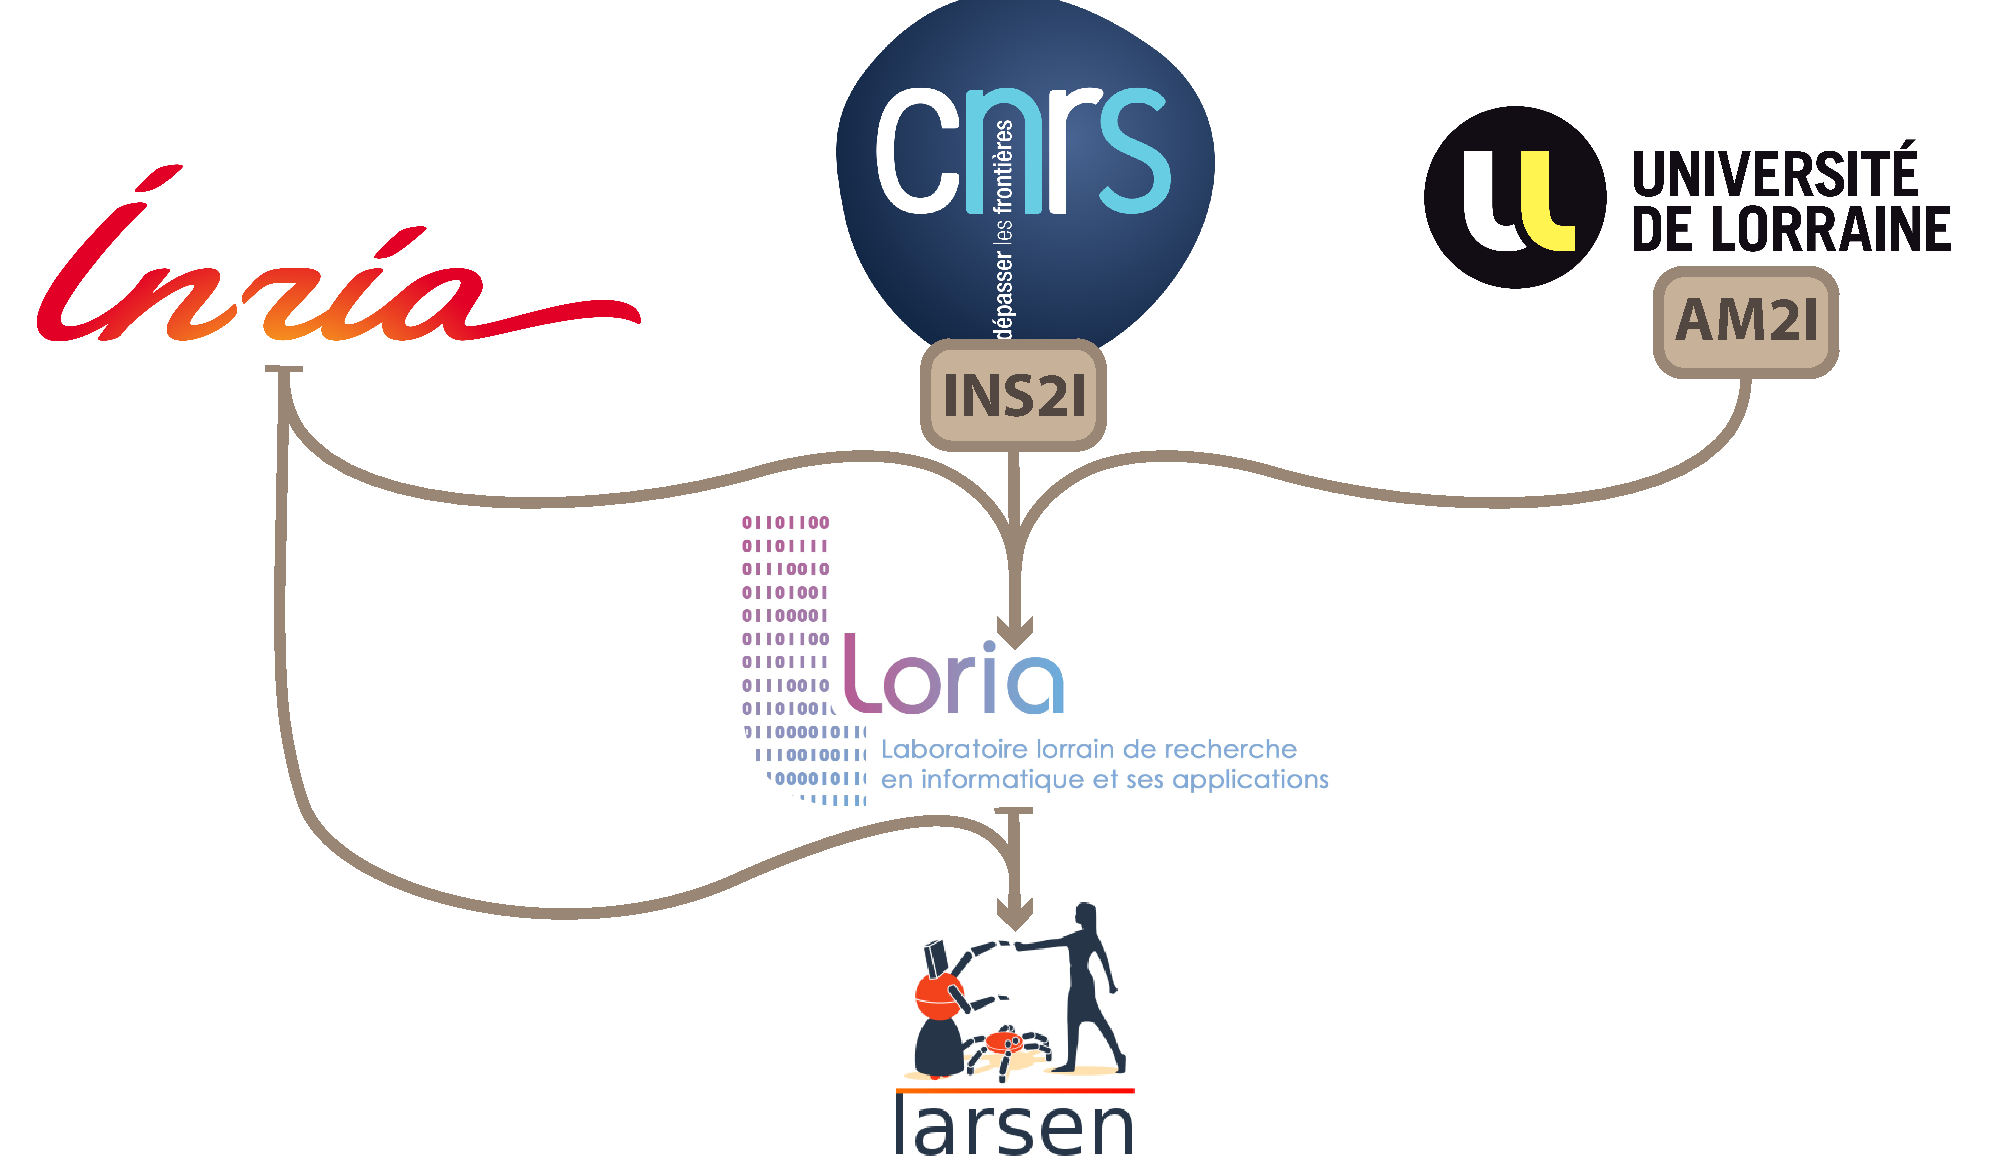
\includegraphics[width = 15cm]{figures/orga_labos}
    \caption{Hiérarchie des entités dont dépend l'équipe \gls{LARSEN}}
    \label{fig:orgaLab}
\end{figure}

\subsection{Centre national de la recherche scientifique (CNRS)}
\subsubsection{Le CNRS en quelques mots}
Le \gls{CNRS} est un \gls{EPST} placé sous la tutelle du ministère de l'éducation nationale, de l'enseignement supérieur et de la recherche. Il a pour objectif de produire du savoir et de le mettre au service de la société. 

Le \gls{CNRS} est présent dans tous les domaines de connaissance. C'est un organisme pluridisciplinaire menant des recherches dans l'ensemble des domaines scientifiques, technologiques et sociétaux.

Ces différentes disciplines sont regroupées au sein de dix instituts:
\begin{itemize}
\item \gls{INSB}   
\item \gls{INC}
\item \gls{INEE}
\item \gls{INSHS}
\item \gls{INS2I}
\item \gls{INSIS}
\item \gls{INSMI}
\item \gls{INP}
\item \gls{IN2P3}
\item \gls{INSU}
\end{itemize}

\vspace{0.5cm}
La sous-structure qui nous intéresse particulièrement, évoquée en \ref{lb:interstructures} est \gls{INS2I}. Cet institut repose sur 49 unités relevant des disciplines informatiques, du traitement du signal, du traitement des images, de l'automatique et de la robotique. L'objectif de cette entité est d'accompagner le développement des sciences informatiques, afin d'en maîtriser les enjeux scientifiques, technologiques et sociétaux.  

\subsubsection{Le CNRS en quelques chiffres}

le \gls{CNRS}, compte près de 32 000 personnes, dont 11 000 chercheurs et 13 500 Ingénieurs, techniciens et administratifs. 

Son budget pour l'année 2015 été de 3,3 milliards d'euros dont 769 millions en ressources propres. 

Le \gls{CNRS} est implanté à travers toute la France, s'appuyant sur 1100 unités de recherche et de service, dont près de 95\% en partenariat avec l'enseignement supérieur.

Le \gls{CNRS}, c'est aussi 1026 entreprises innovantes créées depuis 1999. Et 5629 familles de brevets. 

\clearpage
\subsection{Institut National de Recherche en Informatique et en Automatique (INRIA)}
\subsubsection{INRIA en quelques mots}
\gls{INRIA} est un institut de recherche dédié au numérique et promeut \textit{l'excellence scientifique au service du transfert technologique et de la société}. \gls{INRIA} est organisé en \textit{équipes-projets} qui rassemblent des chercheurs aux compétences complémentaires autour d’un projet scientifique focalisé. Cette organisation induit plus d'ouverture et d'agilité, permettant de mener à bien ses missions avec ses partenaires industriels et académiques. \gls{INRIA} répond ainsi aux enjeux de la transition numérique, à la fois pluridisciplinaires et très applicatifs de la transition numérique en marche. 

\gls{INRIA} transfert vers les entreprises ses innovations devenant ainsi créatrice de valeur et d'emploi, et ce dans de nombreux domaines, allant de la santé à la sécurité, en passant par les transports, l'énergie, et la communication qui, ensemble, formeront l'esquisse de la ville intelligente de demain, ou encore de l'usine du futur.
\subsubsection{INRIA en quelques chiffres}
\gls{INRIA} comporte pas moins de 178 équipes projets, dont 139 en collaboration avec des universités et d'autres établissements de recherche, comme c'est le cas pour l'équipe \gls{LARSEN}.

Ces équipes génèrent 4600 publications scientifiques par an. Dans la même période, 300 thèses sont soutenues.

L'\gls{INRIA} développe aussi de nombreuses relations avec le monde industriel, dans le cadre de sa mission de transfert de connaissances à la société. L'institut détient 390 brevets. 141 logiciels ont été déposés à l'\gls{APP} en 2014. L'\gls{INRIA} a également aidé à la création de 34 start-up depuis 2010.

L'ensemble des ressources de l'\gls{INRIA} est réparti au sein de 8 centres de recherches à travers la France :
\begin{itemize}
    \item Bordeaux
    \item Paris
    \item Rennes
    \item Sophia Antipolis
    \item Grenoble
    \item Nancy (Lieu de déroulement du stage)
    \item Lille
    \item Saclay
\end{itemize}

Enfin, le siège social est situé à Rocquencourt près de Paris. 

Parmi ces ressources, l'on retrouve 2700 collaborateurs de 87 nationalités différentes, dont 1800 scientifiques. 

Le budget total de l'\gls{INRIA} s'élève à 203 M d'euros.


\subsection{Université de lorraine (UL)}

L`\gls{UL} est issue de la fusion de différentes universités existentes le 1er janvier 2012. Les quatre entités fusionnées sont :
\begin{itemize}
    \item  l'Institut national polytechnique de Lorraine
    \item  l'université Henri Poincaré
    \item  l'université Nancy 2
    \item  l'université Paul Verlaine-Metz
\end{itemize}

\vspace{0.5cm}
L'\gls{UL} propose une gamme complète de formations, couvrant de nombreux domaines et coeurs de métiers. Mais outre son rôle d'enseignement supérieur, l'\gls{UL} comporte également une forte composante orientée vers la recherche, qui nous intéresse ici. L'\gls{UL} effectue des recherches dans de nombreux domaines scientifiques, technologiques et sociétaux. 

Ces différentes disciplines sont regroupées au sein de dix pôles scientifiques:
\begin{itemize}
\item \gls{A2F}   
\item \gls{AM2I}
\item \gls{BMS}
\item \gls{CLCS}
\item \gls{CMP}
\item \gls{EMPP}
\item \gls{M4}
\item \gls{OTELo}
\item \gls{SJPEG}
\item \gls{TELL}
\end{itemize}
\vspace{0.5cm}
Le pôle nous concernant est le pôle \gls{AM2I}, qui est une des entités au dessus du \gls{LORIA}.
\subsection{Laboratoire lorrain de recherche en informatique et ses applications (LORIA)}\label{lb:loria}
Le \gls{LORIA} est une Unité Mixte de Recherche (UMR 7503), qui comme évoqué précédemment est commune à plusieurs établissements : le gls\gls{CNRS}, l’\gls{UL} et \gls{INRIA}.

Sa mission principale est la recherche fondamentale mais aussi appliquée en sciences informatiques. Cette mission lui a été assignée dès sa création en 1997.

Le \gls{LORIA} est membre de la Fédération Charles Hermite\footnote{Du nom d'un mathématicien français du XIXe siècle: Charles Hermite, connu pour ses travaux sur la théorie des nombres, les formes quadratiques, les polynômes orthogonaux, les fonctions elliptiques et les équations différentielles.} qui regroupe les trois principaux laboratoires de recherche en mathématiques et en informatique de lorraine. Cette fédération permet au \gls{CRAN}, à l'\gls{IECL} et au \gls{LORIA} de se hisser au 5e rang des centres universitaires nationaux pour les maths-STIC

Le laboratoire comprend un total de 450 personnes, ce qui en fait un des plus grands laboratoires de la région Lorraine. Les différents projets du laboratoire sont menés par 30 équipes, dont 15 communes avec \gls{INRIA}.

Ces équipes sont organisées en 5 départements, comme le montre la figure \ref{fig:orgaLoria}. L'équipe \gls{LARSEN} est intégrée dans le département 5 : \textit{  Systèmes complexes, intelligence  
  artificielle et robotique }.
\section{Présentation de l'équipe}\label{lb:larsen}

L'équipe \gls{LARSEN} a été créée le 1er janvier 2015 à \gls{INRIA} Nancy.

L'objectif de l'équipe est d'amener les robots ailleurs que dans des laboratoires de recherche et les industries. Pour atteindre cet objectif, l'équipe \gls{LARSEN} développe des méthodes pour offrir une autonomie à long terme ainsi qu'une capacité d'interaction au robots, prenant en compte des capteurs embarqués ou externes placés dans l'environnement.

Ces capacités sont regroupées autour de l'interaction physique et sociale, de l'apprentissage et du planning gérant l'incertitude. Les expérimentations, concernant particulièrement le service et les robots d'assistance, sont au coeur de la méthodologie de l'équipe. 

Les techniques développées par l'équipe vont potentiellement impacter le domaine de la robotique et ainsi catalyser les efforts afin de transférer les robots au sein de notre société 
\subsection{Organigramme}
\begin{figure}[h]
    \centering
    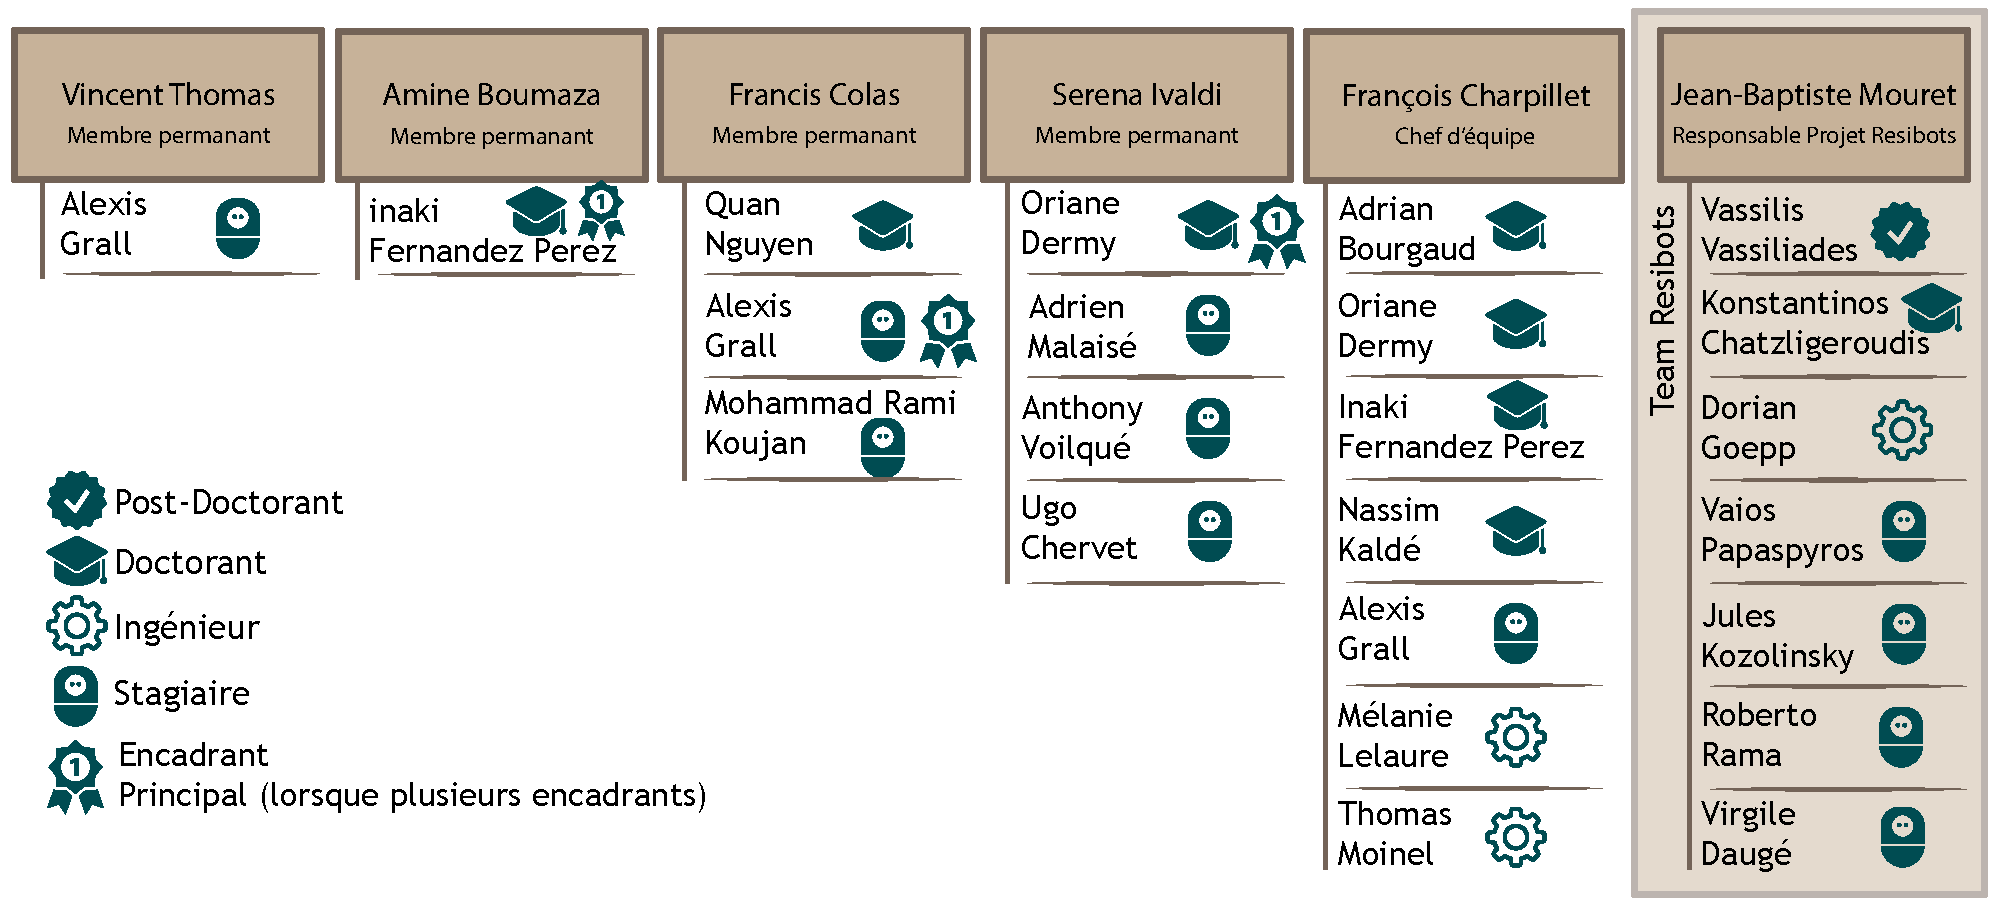
\includegraphics[width = 17.5cm]{figures/team}
    \caption{Les membres de l'équipe LARSEN}
    \label{fig:team}
\end{figure}
\subsection{Resibots}

Le projet resibot est un projet européen, porté par Jean-Baptiste Mouret, et financé depuis 2015 pour une période de 5 ans par \gls{ERC}. Il a pour but de combler les lacunes actuelles des robots en terme d'adaptation. En effet, à l'heure actuelle, malgré de nombreuses années de recherches dans le domaine, les robots sont toujours des machines fragiles, qui peuvent facilement s'arrêter de fonctionner lorsqu'elles subissent des imprévus.

L'objectif du projet est de fournir une base algorithmique pour la réalisation de robots économiques, capables de récupérer de dommages imprévus en quelques minutes. 

L'approche actuelle de la tolérance aux pannes est héritée des systèmes critiques de sécurité (par exemple des vaisseaux spatiaux ou des centrales nucléaires ) . Elle est inappropriée pour les robots autonomes à faible coût car elle repose sur des procédures de diagnostics, qui nécessitent des capteurs proprioceptifs\footnote{Des capteurs proprioceptifs permettent de connaître les caractéristiques intrinsèques du robot comme la position de ses membres, les couples appliqués par ses moteurs etc... il permettent donc d'avoir une connaissance avancée de son état actuel.} coûteux, et des plans d'urgence, qui ne peuvent pas couvrir toutes les situations possibles qu'un robot autonome peut rencontrer.

Il est ici soutenu que les algorithmes d'essais et erreurs par apprentissage offrent une approche alternative qui ne nécessite pas de diagnostic, ni de plans d'urgence pré-établis. Dans ce projet, l'équipe développe et étudie une nouvelle famille d'algorithmes d'apprentissage permettant aux robots autonomes de découvrir rapidement les comportements compensant les imprévus. Les techniques développées dans ce projet augmenteront sensiblement la durée de vie des robots sans augmenter leur coût et permettront d'ouvrir de nouvelles pistes de recherche pour les machines adaptatives.



\chapter{État de l'art}

Rappelons la problématique de réalisation d'un contrôleur réactif prenant en compte les capteurs de forces aux extrémités des pattes. Afin de répondre au mieux à la problématique posée, il est nécessaire d'effectuer des recherches. L'idée était ici dans un premier temps de faire le tour des différentes approches actuellement utilisées, leurs résultats et enfin, si ces derniers paraissent concluants, d'étudier voire réaliser l'implémentation de l'approche prometteuse. 

Il existe de nombreuses approches, mais il convient de les différencier en deux grande catégories avec des objectifs différents. La première sera présentée en \ref{lb:biomimetic} et concerne les approches biomimétiques, qui n'ont pas forcément pour but principal d'aboutir à une solution performante, mais plus de découvrir de nouvelles façon de procéder, inspirées du vivant. La seconde, abordée en \ref{lb:pratique} regroupe quant à elle des approches plus classiques sinon plus pragmatiques.  

\section{Méthode et outils}
Il existe de nombreuses publications liées directement ou indirectement aux objectifs du stage. Afin d'être capable d'extraire des informations cohérentes et exploitables de cette masse de données, il était nécessaire d'adopter une méthode efficace afin d'éviter de perdre beaucoup de temps dans cette phase préparatoire. L'objectif de cette section est donc de présenter la méthode adoptée, ainsi que les outils utilisés au sein de cette méthode afin de faciliter le stockage et le tri des publications 

\subsection{Méthode}
\subsubsection{Accès aux informations}
La phase de recherche de publications s'est effectuée principalement sur l'outil \textit{Google Scholar} présenté en \ref{lb:googleScholar}. Afin de trouver des articles connexes, et intéressants vis-à-vis de la problématique du stage, il a fallu utiliser des mots-clés pertinents. 
 
L'accès à la plupart des publications scientifiques connexes était fourni et donc payé par l'\gls{INRIA}. Certaines n'étaient néanmoins pas accessibles, et sans avoir à l'avance une idée fondée sur leur potentielle pertinence, il a fallu s'en passer. La richesse du catalogue de l'\gls{INRIA} a tout de même permis de toucher un panel important de publications, cette limitation étant survenue un nombre très faible de fois. 

Afin de conserver les références des publications trouvées, l'utilisation d'un outil spécialisé a permis de gagner beaucoup de temps. Plusieurs outils de ce type existent, j'ai choisi d'utiliser \textit{Zotero} outil présenté en \ref{lb:zotero}.

Une fois une publication connexe trouvée, il convient bien entendu de l'analyser, voyons maintenant comment.

\subsubsection{Lecture rapide}
Au vu du nombre important de publications dans le domaine visé, et de la particularité de la problématique du stage, il est primordial d'essayer d'évaluer la pertinence d'un papier dans le contexte précis de la réalisation demandée avant d'en lire tous les détails. C'est pour cette raison qu'une lecture rapide est préférable à une lecture approfondie dans un premier temps. 

L'objectif de cette lecture rapide, est d'essayer de cerner plusieurs points dans la publication. De prime abord, il s'agit de comprendre le concept évoqué. Cela revient à répondre aux questions suivantes :
\begin{itemize}
    \item Que font-ils globalement ?
    \item Quels objectifs se sont-ils fixés ?
    \item Quelle approche est mise en avant ?
\end{itemize}    

Ces éléments permettront par la suite de classer les différentes publications en catégories, afin de pouvoir retrouver facilement les informations concernant chaque approche. Cette partie est abordée en \ref{lb:classification}.

Maintenant que l'on a déterminé l'approche du papier, il est important d'en évaluer rapidement la pertinence. Il s'agit donc de trouver les résultats parfois quantifiés qui sont souvent mis en avant vers la fin de la publication. En effet, l'approche peu paraître vraiment intelligente et intéressante mais finalement s'avérer décevante en termes de résultats pratiques. 

Cette brève analyse des résultats est parfois difficile à effectuer car les résultats présentés sont dans certains cas incomplets, et souvent à l'avantage de la méthode. Ce qui est dans une certaine mesure légitime, mais qui peut vite s'avérer problématique, par exemple si les résultats proposés omettent un paramètre important pour notre projet. 

C'est pourquoi il est bon de se baser sur d'autres sources que les publications elles-mêmes pour établir notre première impression sur les performances réelles d'une solution. 
\clearpage
\subsubsection{Vidéos}
Un des avantages de la robotique, est le côté très visuel des choses. En effet, que l'on travaille en simulation ou directement sur un robot, il est possible d'analyser rapidement la performance d'un comportement simplement en regardant le robot effectuer ses commandes. Cela permet finalement, dans un contexte d'évaluation rapide et globale, de prendre en compte aisément de nombreuses variables, qui seraient certainement moins évidentes à appréhender dans un autre domaine moins visuel.

Vous l'aurez compris, une vidéo en dit long sur le comportement d'un robot, et présente l'intérêt de permettre moins de libertés concernant la mise en avant des résultats arrangeants. Bien qu’il soit toujours possible de réaliser une expérience dans des conditions idéales, on peut assez facilement voir par exemple qu'il n'y a pas d'obstacles, où que ces derniers sont dimensionnés pour faciliter leur franchissement en accord avec la géométrie et les capacités du robot testé. Cela donne donc souvent une idée du meilleur comportement atteignable par cette méthode, ce qui reste une information intéressante. 

Lorsque le lien entre la vidéo et la publication est explicite, c'est un très bon moyen d'évaluation rapide des performances d'un algorithme. Dans les autres cas, il faut réellement être prudents sur les conclusions tirées du visionnage d'une vidéo. 

\subsubsection{Classification} \label{lb:classification}
La Classification des méthodes de contrôle n'a pas été aisée, car elles opèrent souvent à des niveaux différents. Certaines méthodes issues d'une catégorie seront donc amenées à être utilisées conjointement avec des méthodes issues d'autres catégories opérant à un autre niveau. 

\subsubsection{Lecture approfondie}
Une fois la publication jugée suffisamment pertinente selon les méthodes rapides présentées précédemment, puis assignée à une catégorie, il convient de l'analyser plus en détail. L'idée est ici d'aller chercher dans les détails de la publication la compatibilité entre la méthode proposée et la problématique imposée. 

En effet, de nombreuses raisons peuvent rendre incompatibles un algorithme avec la plateforme réelle du projet. Par exemple une méthode exploitant un degré de liberté élevé de chaque patte \footnote{supérieur aux 3 degrés de libertés généralement disponibles sur les pattes d'un hexapode et sur notre hexapode.}, qui pose problème si l'on ne dispose pas de pattes avec un degré de libertés suffisant. De manière plus générale si le robot utilisé comme plateforme d'expérimentation à une géométrie différente de celui sur lequel on travaille, et que l'un des concepts de la méthode proposée dans le papier s'appuie sur cette particularité physique. C'est le cas par exemple pour le robot \textit{RHex}\cite{saranli_rhex:_2001} qui a des pattes tournantes, et qui se contrôle par conséquent d'une manière diamétralement opposée à un hexapode classique. 

Il est parfois ardu de comprendre l'intégralité d'une publication lors de la première lecture approfondie, cela entraîne quelques fois des lectures en cascade, une publication s'appuyant souvent sur un travail préliminaire déjà publié. Cette étape à donc consommé beaucoup de temps et d'énergie, au vu du nombre de publications disponibles.

\subsection{Outils}
La construction d'un état de l'art requiert une solide organisation, qui est rendue possible par l'emploi de nombreux outils. Il ne s'agit bien évidemment pas de présenter ici  tous les outils utilisés mais de traiter les principaux, qui seront essentiels à la réalisation d'un état de l'art convenable.  
\subsubsection{Google Scholar}\label{lb:googleScholar}
Google Scholar est un service de recherche d'articles universitaires, de thèse ou encore de livres scientifiques. Lancé en 2004, le service de Google prétendait déjà couvrir 85\% des publications scientifiques. Il reste cependant difficile d'évaluer réellement sa couverture des oeuvres existante. En effet, même s'il est avéré qu'il se base sur des éditeurs scientifiques, et des serveurs universitaires, aucune mention précise de ses sources n'est effectuée. 

Cependant, certaines informations comme les travaux réalisés par des amateurs, souvent relayées via des blogs spécialisés, ne sont pas indexées ici. Ces sources supplémentaires peuvent parfois s'avérer utile, notamment car elles font la part-belle aux détails de l'implémentation, souvent relayée au second plan dans les publications scientifiques. 

\subsubsection{Zotero} \label{lb:zotero}
Au vu du nombre de publications à couvrir, l'utilisation d'un outil d'archivage était indispensable. Il existe de nombreuses solutions disponibles remplissant le rôle de collecte, d'organisation de citations ou encore d'export de sources.

Parmi ces nombreuses solutions, parfois payantes, Zotero et Mendeley se démarquent par leur complétude et leur gratuité. Il proposent tous deux les fonctionnalités indispensables. Après avoir brièvement testé les deux concurrents, la facilité d'utilisation de Zotero due à son intégration dans le navigateur Web Firefox m'a conquis.

Cet outil est vraiment pratique, car en plus de la possibilité de stocker et de trier les publications enregistrables en un seul clic, ce dernier permet également d'exporter une bibliothèque sous divers formats. L'intérêt principal de cet export est le format bibTex, utilisé par la suite lors de la rédaction de ce rapport. Ayant de nombreuses références, c'est un gain de temps non négligeable.  

\newpage
\section{Approches Biomimétiques}\label{lb:biomimetic}
S'inspirer de la nature et du vivant pour concevoir de nouveaux types de contrôleur robotiques est en vogue actuellement. Il existe de très nombreuses expérimentations, principalement basées sur des \glspl{réseau neuronal}\footnote{\glsdesc{réseau neuronal}}.

Les travaux présentés ici tentent de résumer brièvement et au mieux l'ensemble des approches de contrôles biomimétiques trouvées concernant des hexapodes. Ce n'est donc pas une liste exhaustive, et elle concerne uniquement les travaux accessibles lors de l'été 2016, date de réalisation du stage. 
\subsection{Le vivant comme inspiration}
L'objectif des recherches présentées ici est ambivalent. En effet, il ne s'agit pas uniquement de mimer le comportement animal pour trouver un contrôleur efficace, mais il s'agit également de prouver qu'il est possible d'arriver à un contrôleur via ces approches. Pour reformuler plus clairement, atteindre un contrôleur performant est souhaitable, mais prouver qu'il est possible de copier le monde animal l'est tout autant.

L'intérêt de ces approches biomimétiques, comme le souligne une publication relativement ancienne de Cynthia Ferrell \cite{ferrell_comparison_1995}, réside dans la robustesse, l'adaptivité et le caractère versatile de la locomotion animale, notamment de celle des insectes. 

L'intérêt de cette publication est qu'elle compare différentes approches, fait rare dans les publication que j'ai eu l'occasion de lire. La plupart se contentant de proposer leur approche, mettant en avant leurs résultats sans vraiment détailler les conditions des expérimentations.


\subsection{Réseaux de neurones}

\subsubsection{Pourquoi les utiliser ?}
Il est connu que le cerveau humain ou animal est capable de réaliser certaines tâches complexes aussi bien que le plus avancé des ordinateurs. Les phasmes sont par exemple capables de résoudre le problème complexe que pose la marche à l'aide d'un réseau de neurones relativement simple. Des modèles inspirés de la nature appelés réseaux de neurones artificiels (Artificial Neural Network ou ANN en anglais) ont été développés.  

\subsubsection{Les avantages de leur emploi}
L'avantage principal des réseaux de neurones réside dans leur capacité d'adaptation. Un même réseau peut en effet accomplir une tache en s'adaptant à de nombreuses configurations différentes. Il est en revanche nécessaire de l'entraîner pour chacune de ces configurations. Les avantages d'un système basé sur un réseau de neurones sont les suivants :
\begin{itemize}
    \item Ils peuvent potentiellement gérer une grande quantité de données avec une grande précision;
    \item Ils sont potentiellement robustes au bruit, erreurs et autres perturbations;
    \item Leur caractéristiques non-linéaires, distribuées, parallèles permettent d'en augmenter la performance.
\end{itemize}
\vspace{0.5cm}
Leur particularité réside dans le fait qu'ils peuvent apprennent de leur expérience. Comme énoncé précédemment, il faut les entraîner afin de leur permettre de trouver les bons paramètres permettant de réaliser correctement la tâche qui leur est affectée. L'inconvénient de ces systèmes et qu'il est difficile de les analyser, ils doivent donc être souvent considérés comme des boites noires. 

\subsubsection{Structure}
Un ANN est constitué de noeuds, appelés neurones artificiels, qui échangent des informations entre eux à travers des connexions appelés synapses. Chaque neurone est défini par une entrée, une fonction d'activation, un biais d'activation ainsi qu'une sortie. 

Chaque synapse reliant deux neurones est caractérisé par un poids. Le biais de chaque neurone ainsi que le poids de chaque synapse sont les paramètres à trouver. La fonction d'activation est bien souvent une simple fonction de seuil. 

Cela peut paraître simple, mais en pratique les réseaux sont souvent complexes. Pour la reconnaissance d'images par exemple, plusieurs dizaines voire centaines de couches cachées peuvent êtres utilisées. Cela augmente donc considérablement le temps et les données nécessaires pour l'entraînement de l'ANN. 

Sans aller si loin, en restant dans le contexte d'un contrôleur d'hexapode, certains exemples comme celui tiré de la publication de Manoonpong \& Al\cite{manoonpong_sensor-driven_2008} visible sur la figure \ref{fig:manoonarchi} sont déjà avancés. Cette publication n'est pas unique en son genre et de nombreuses solutions du même type existent, chacun essayant des variantes afin de rendre le système plus performant. Nous allons donc maintenant aborder le fonctionnement de ce contrôleur.

\subsubsection{Un exemple détaillé}
Nous pouvons remarquer la présence de divers groupes de neurones différents sur la figure \ref{fig:manoonarchi}. Ils sont ici au nombre de trois :
\begin{itemize}
    \item Un groupe \gls{CPG}
    \item Un groupe \gls{PSN}
    \item Un groupe \gls{VRN}
\end{itemize}

\begin{figure}[h]
    \centering
    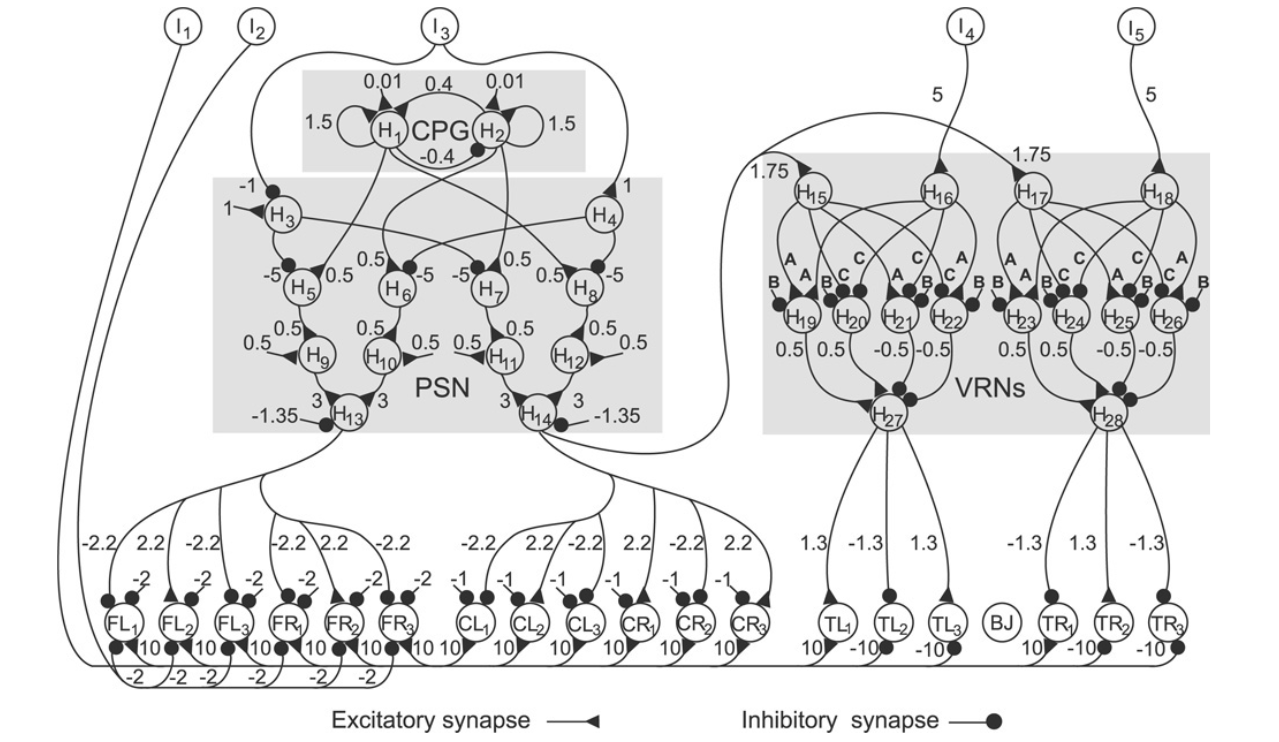
\includegraphics[width =\textwidth]{figures/mannoonarchi}
    \caption{Exemple de réseau de neurones d'un contrôleur \cite{manoonpong_sensor-driven_2008}}
    \label{fig:manoonarchi}
\end{figure}

Le premier (\gls{CPG}) a pour but de générer une fréquence désirée afin de synchroniser la marche. Il est relativement simple, et ses poids on été déterminés de manière empirique. 

Le second, (\gls{PSN}) doit quant à lui déterminer la phase de la patte : doit-elle supporter le poids ou avancer ? Il utilise pour cela la fréquence créée précédemment, ainsi que le neurone d'entrée $I_3$, qui servira à commander le sens des déplacements latéraux et diagonaux. Ses neurones de sortie contrôlent les servomoteurs des genoux et chevilles. Il a été construit à la main et ses poids choisis empiriquement. 

Enfin, le troisième groupe, nommé \gls{VRN} sert à contrôler la vitesse de la marche. Il se sert de la fréquence initialement générée par le premier et traitée par le second groupe afin de maintenir la vitesse désirée. Ainsi que des entrées $I_4$ et $I_5$ afin de déterminer le sens de la marche --Avant, arrière, tourner à droite, tourner à gauche...-- en jouant sur le signe de ses derniers. Modifier leur amplitude augmentera la vitesse de marche. Ses neurones de sortie contrôlent quant à eux les servomoteurs des hanches. 

La correspondance entre les neurones de sortie et les servomoteurs est donnée en figure \ref{fig:manoonarchi2}. 

\begin{figure}[h]
    \centering
    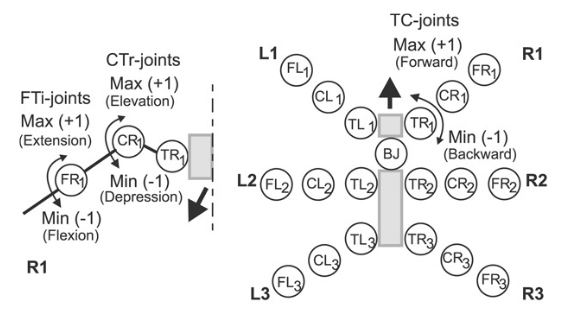
\includegraphics[width = 15cm]{figures/mannoonarchi2}
    \caption{Lien avec les servomoteurs\cite{manoonpong_sensor-driven_2008}}
    \label{fig:manoonarchi2}
\end{figure}

\subsection{Plusieurs niveaux de commande}

Si certains travaux comme ceux évoqués précédemment\cite{manoonpong_sensor-driven_2008} utilisent un réseau de neurones comprenant le contrôle simultané de toutes les pattes ainsi que leur synchronisation, d'autres travaux qui seront brièvement évoqués en \ref{lb:rsltpastop} comportent quant à eux une approche de contrôle indépendant de chaque patte. Ce type d'approche parait plus intéressant, bien qu'il faille certainement entraîner chaque patte en fonction de sa position sur le corps, et qu'il faille également intégrer un mécanisme de synchronisation. 

Il est dans tous les cas nécessaire d'implémenter un mécanisme de contrôle des pattes ainsi qu'un mécanisme de synchronisation de ces dernières, les deux pouvant êtres plus ou moins liés.

\subsection{Des comportements adaptatifs}

L'entraînement doit se faire sur un set de données suffisantes, mais pas trop non plus, sans quoi on risque un surentraînement et le robot ne sera plus capable de généraliser et donc de s'adapter à des situations inconnues. Ce problème survient lorsque durant l'entraînement, l'on expose toujours le robot aux mêmes types d'environnements ou d'obstacles. Petit à petit, il va apprendre à gérer au mieux cet obstacle, jusqu'à potentiellement avoir un comportement optimal pour celui-ci. On peut même parler de comportement spécialisé pour cet obstacle. Il va donc prendre des habitudes qui fonctionnent bien dans ce cas précis, mais qui vont affaiblir le comportement du robot lorsqu'il se retrouvera dans un contexte différent. Il essaiera alors d'appliquer ces routines qui fonctionnaient si bien dans un contexte totalement inapproprié. 
\clearpage

Même dans le cas d'une détermination manuelle et empirique des poids des synapses, il n'est pas garanti que le robot soit réellement capable de s'adapter à un cas particulier, non testé préalablement. 

Les comportement adaptatifs, grandement mis en avant dans certaines publications ne concernent souvent que des variations mineures de l'environnent. Ainsi le robot bipède \textit{runbot} dont le contrôleur est présenté de la publication \textit{Adaptive, Fast Walking in a Biped Robot under Neuronal Control and Learning} \cite{manoonpong_runbot_2007}, est capable de ne pas tomber lorsqu'il rencontre une rampe inclinée à 8° par rapport au reste du sol. 

\subsection{Des résultats décevants}\label{lb:rsltpastop}

Après avoir lu de nombreuses publications concernant ce type de contrôleurs (\cite{ren_multiple_2015}, \cite{santos_cpg_2012} et d'autres) les résultats obtenus étaient souvent décevants au vu de la complexité du travail présenté. Après avoir visualisé quelques vidéos correspondantes sur Youtube, l'enthousiasme crée lors de la lecture des publications s'estompait rapidement.

En revanches d'autres approches paraissent plus prometteuses, comme celle présentée dans la publication récente \textit{Adaptive and robust leg control of a
hexapod robot for space exploration}\cite{travaglini_adaptive_2015}. En effet, après avoir entraîné leur contrôleur de patte sur un terrain plat, celui ci reste robuste sur un terrain plus chaotique ou encore sur une pente. Ces résultats encourageants ne sont malheureusement pas suffisants pour opter pour cette approche, les travaux et expérimentations ayant été conduits sur une seule patte. Le contrôleur complet devrait être réalisé, mais à l'heure actuelle, rien ne permet d'affirmer que cette approche fonctionnera bel et bien une fois généralisée. De plus, cette approche prend en compte les retours des capteurs, mais très faiblement, et évite de développer cet aspect, qui est rappelons le au centre de la problématique de ce stage. 

\subsection{Une approche inadaptée}

De premier abord, une approche basée sur un réseau neuronal parait intéressante. En effet, l'idée de construire un contrôleur simplement en s'inspirant voire en copiant une publication présentant son réseau de neurone peut paraître rapide et efficace. En réalité, le contrôleur sera rapidement implémenté, mais il nécessitera de très nombreux réglages, afin d'affiner les poids des différents synapses afin de l'adapter à notre robot. 

Si l'on effectue un rapide bilan, peu d'approches biomimétiques donnent à l'heure actuelle une réelle importance aux capteurs, peu d'approches biomimétiques sont réellement robustes, peu d'approches biomimétiques proposent des résultats convainquants. 

Si on ajoute l'importante difficulté de la mise en place d'un tel système, de son entraînement et le temps disponible pour mener à bien les objectifs du stage, opter pour une approche biomimétique ne semble pas être optimal.  

\newpage
\section{Approches plus pragmatiques}\label{lb:pratique}
Nous avons vu des solutions s'inspirant du vivant et copiant le vivant jusque dans la façon de procéder. Abordons maintenant des solutions plus pragmatiques, parfois inspirées de la nature, mais basées cette fois ci sur un socle de connaissances bien connu que forment la mécanique, l'automatique ou encore la physique.

Contrairement aux approches biomimétiques étudiées précédemment, les approches plus pragmatiques diffèrent tant dans leur logique que dans le niveau -- contrôle d'une patte uniquement, planning, synchronisation des pattes etc -- ce qui les rends parfois incompatibles et parfois complémentaires

A contrario des réseaux de neurones qui contrôlent tout les aspects de la marche à la manière d'une boite noire, il est ici nécessaire de maîtriser toutes les étapes nécessaires au bon fonctionnement du contrôleur dans son ensemble.
\subsection{Le contrôle basé sur des pattes indépendantes}
L'intérêt de contrôler les pattes séparément est double pour nous. En effet, en dehors des considérations traditionnelles que sont le découplage et la capacité de réflexe local, l'équipe resibots travaille sur des robots endommagés, avec un nombre de pattes variable. Ce type de contrôleur parait d'emblée plus adapté à notre problématique. 

\subsubsection{Contrôle de trajectoire}

C'est un thème peu voire pas abordé dans les publications scientifiques concernant les robots marcheurs. Globalement, soit l'on opte pour une logique de contrôle par position des moteurs, qui présente l'avantage d'être simple de mise en oeuvre et sûr. Cela représente néanmoins l'inconvénient de devoir penser nos mouvements selon la position angulaire des moteurs, ce qui n'est pas réellement naturel. 

C'est une solution qui peut sembler suffisante dans un premier temps, mais qui montrera ses limites lorsque le besoin de trajectoires complexes se fera ressentir. 

L'autre solution disponible est de travailler en logique cartésienne --c'est à dire de penser aux points que doit atteindre l'extrémité de la patte-- puis de convertir ces points objectifs en commandes moteurs grâce à la cinématique. Cette solution sera retenue car malgré son éventuelle complexité de mise en oeuvre, elle permettra par la suite une grande liberté dans la génération des trajectoires de la patte. Elle sera présentée plus en détail dans la section \ref{lb:kinematics}. 

\newpage
\subsubsection{Contrôle de la force}\label{lb:ctrlforce}

Le contrôle de la force se base sur différents types de capteurs, plus ou moins précis, mais donnant tous une idée de la force appliquée à l'extrémité de la patte. L'exemple le plus simple est présenté dans la publication \textit{Force Threshold-Based Omni-directional Movement for Hexapod Robot Walking on Uneven Terrain}\cite{irawan_force_2012} semble être un bon point de départ. 

Il s'agit ici de stopper le mouvement de la patte lors de la détection d'un contact avec un éventuel obstacle. L'objectif est d'éviter au robot de forcer sur cette patte après le contact, ce qui permet à la fois d'éviter que cette patte supporte une trop forte charge, et d'éviter que ce mouvement ne renverse ou déstabilise le robot. 

Cette détection se fait grâce à un simple seuil de force. Une fois la force appliquée à l'extrémité jugée suffisante -- au dessus du seuil fixé -- on stoppe le mouvement et passe la patte en mode support, cessant alors de déstabiliser le robot et suivant son mouvement tout en servant d'appui. On passe donc grâce à ce procédé d'un comportement diminuant la stabilité du robot à un comportement l'augmentant. 

En affinant ce principe, il est possible de maîtriser la force de contact de chaque pied. C'est à dire d'adapter la position et posture de la patte afin de maintenir une pression constante. Cette possibilité est mise en avant dans la publication \cite{irawana_adaptive_2014}. 

Cela apporte plusieurs avantages, d'une part, il est possible non seulement de s'assurer d'une portance suffisante, mais également d'éviter de trop forcer sur une seule patte évitant de l'enfoncer dans un sol meuble. C'est tout à fait approprié dans le cadre de leur étude, visant à faire marcher un hexapode au fond de l'océan. Dans tous les cas, l'apport de la maîtrise des forces appliquées est un apport conséquent et permet d'utiliser des techniques de synchronisation et de positionnement globales plus évoluées. C'est donc une solution vers laquelle on devrait tendre à terme. 

\subsubsection{Synchronisation entre les pattes}
La synchronisation peut être totalement indépendante, mais est toutefois nécessaire afin d'obtenir un comportement cohérent. Il existe différents mécanismes de synchronisation, plus ou moins compliqués, souvent basé sur un \textit{duty factor} de chaque patte, indiquant quelle proportion du temps celle-ci doit être posée. La synchronisation n'est pas au coeur de la problématique du stage, on peut donc se permettre de mettre en place un mécanisme de synchronisation simple, en permettant toutefois une certaine souplesse permettant de le remplacer facilement. 

Le modèle choisit est un \textit{tripod gait}, déplaçant 3 pattes lorsque les 3 autres sont en contact avec le sol. Il est simple à implémenter, et comporte l'avantage d'être toujours stable car la projection du centre de masse se trouve toujours dans le triangle de support formé par les pattes, comme illustré par la figure \ref{fig:tripod}.

\begin{figure}
    \centering
    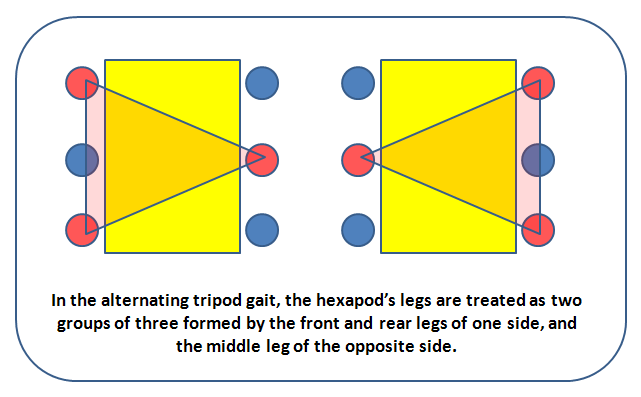
\includegraphics[width=\textwidth]{figures/tripod}
    \caption{La marche tripod}
    \label{fig:tripod}
\end{figure}

\subsection{Le contrôle complet du robot}
Une fois les pattes capables d'exécuter un déplacement précis, de maintenir une force désirée sur une position choisie, il devient possible de contrôler le robot à un plus haut niveau.

\subsubsection{Contrôle omnidirectionnel}

Proposer un contrôleur omnidirectionnel permet de révéler tous les avantages d'un robot sur pattes. Le papier \textit{Towards Omnidirectional Locomotion Strategy 
for Hexapod Walking Robot} \cite{seljanko_towards_2011} présente différentes stratégies pour réaliser un contrôleur omnidirectionnel. Il présente en revanche des approches plus haut niveau, permettant par exemple d'éviter des obstacle. Notre contrôleur n'a pas vocation à évoluer à si haut niveau, il sera donc préférable d'implémenter uniquement la fonctionnalité de base permettant de se déplacer dans toutes les directions sans considération d'évitement. 

\subsubsection{Center Of Mass}
L'approche basée sur le \gls{CoM} permet d'augmenter la stabilité du robot. L'idée est de déplacer ce dernier en fonction des perturbations extérieures subies afin d'augmenter la stabilité du robot. On doit donc connaître la posture actuelle du robot ainsi que les forces qui lui sont appliquées. Cela est possible dans notre cas grâce aux codeurs de positions dont sont équipés les servomoteurs et des capteurs de force placés à l'extrémité de chaque patte.

La publication \textit{Foot Force Based Reactive Stability of Multi-Legged Robots
to External Perturbations} \cite{agheli_foot_2015} explique bien ce concept, et propose de calculer une carte des forces appliquées aux pattes afin de déterminer les perturbations extérieures, puis de les compenser soi en bougeant le centre de masse (auquel ils font référence sous le terme de centre de gravité : CG). Si changer la position du centre de masse sans bouger les extrémités des pattes ne suffit pas ils bougent ses extrémités afin de compenser au mieux. Ce schéma décisionnel est illustré par la figure \ref{fig:comdec}.

\begin{figure}
    \centering
    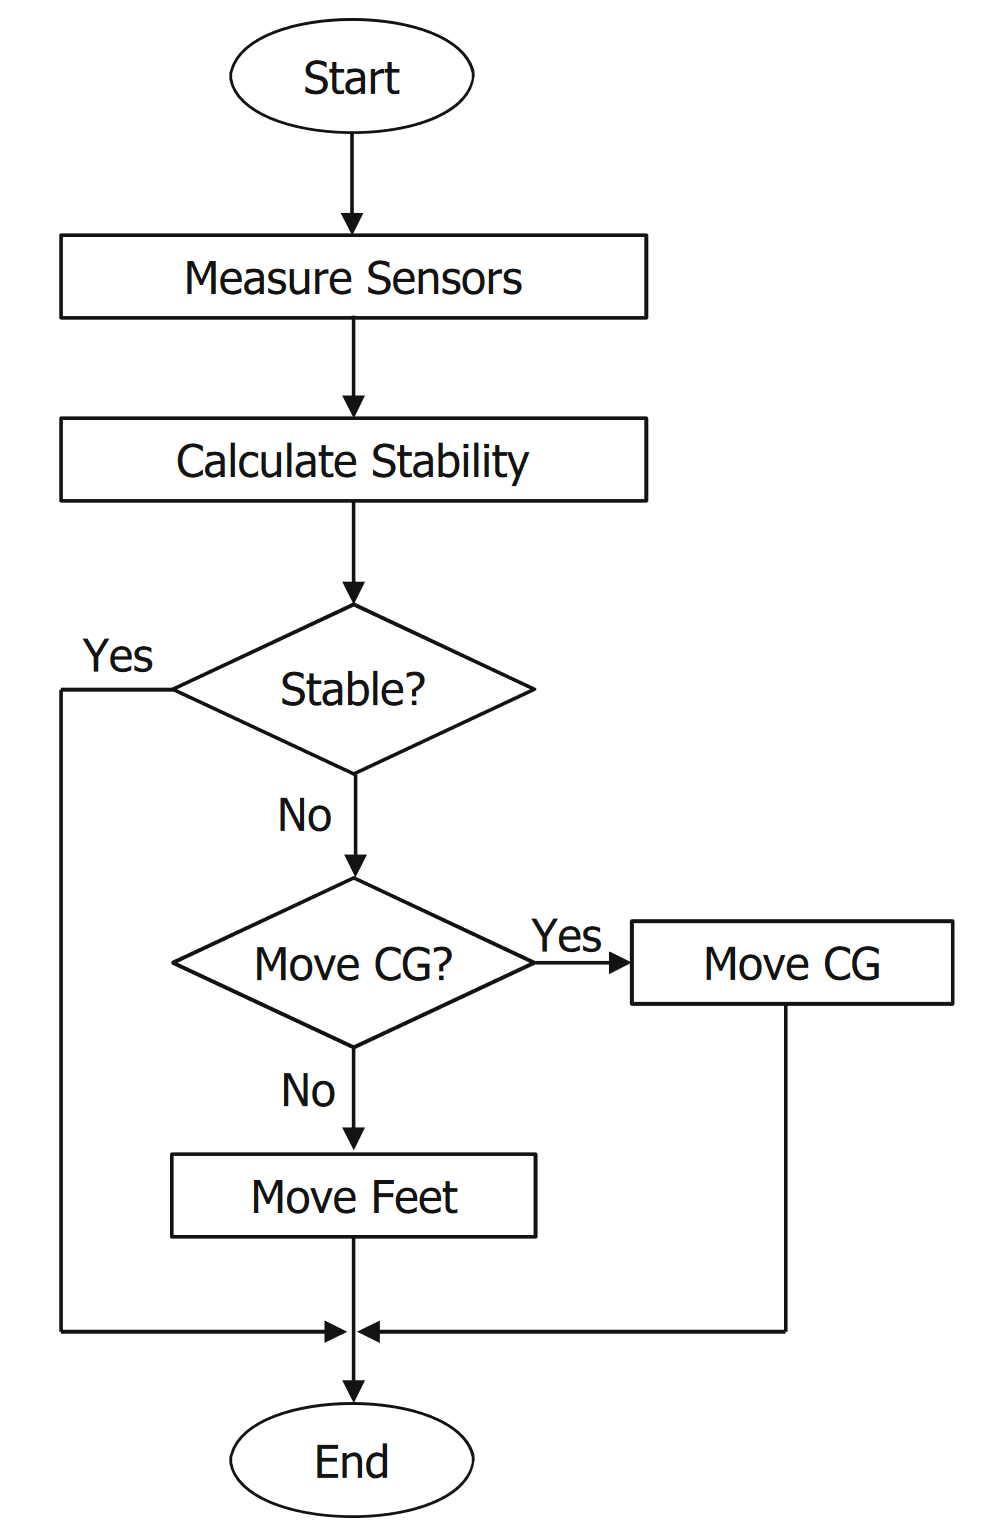
\includegraphics[scale=0.6]{figures/com}
    \caption{Logique décisionnelle de l'approche basée sur le \gls{CoM}}
    \label{fig:comdec}
\end{figure}

\subsubsection{\gls{MPC}}
Une autre approche consiste à utiliser une méthode maîtrisée et bien connue empruntée à l'automatique. L'idée est de posséder un modèle complet du robot, afin de pouvoir calculer l'impact d'une action sur ce système. 

Ces conséquences sont souvent calculées sur plusieurs périodes de contrôle, afin d'avoir une idée des conséquences à long terme de l'action testée. la décision est ensuite prise d'effectuer ou non cette action sur la prochaine période de contrôle. 

Puis on réitère l'opération à la fin de cette période. La publication récente \textit{A Reactive Walking Pattern Generator Based on Nonlinear Model Predictive Control} \cite{naveau_reactive_2016} détaille son emploi. Les capacités de cette approche semblent prometteuses. 

Le soucis qui se pose ici et que si l'on maîtrise le modèle du robot, on ne connaît en revanche pas le terrain dans lequel il évolue. Il est donc difficile de prévoir le résultat d'une commande. Si, lors de la marche, l'on décide de poser le pied, le résultat final de cette action dépend de ce qui se trouve réellement au point de contact. 

Sans un modèle de l'environnement, il parait donc difficile de construire un contrôleur stable et robuste, en utilisant un \gls{MPC}. Il faudrait alors y intégrer la notion d'incertitude afin de le rendre l'ensemble fonctionnel. Cela représente donc une possible évolution de notre contrôleur, mais semble un peu audacieuse pour une première version. 

C'est la raison pour laquelle nous n'allons pas nous diriger dans cette voie pour l'instant. Opter pour une approche plus simple basée sur un simple seuil de force, couplé à des calculs cinématiques et un contrôleur omnidirectionnel paraît être une solution plus raisonnable étant donné les contraintes de temps et l'inéxpérimentation du stagiaire en la matière. 

\chapter{Architecture}

L'objectif de ce chapitre est de présenter les éléments nécessaires à la compréhension du travail réalisé qui sera présenté en \ref{lb:travail}. L'idée est de présenter dans un premier temps le matériel utilisé notamment la plateforme robotique sur laquelle sera implémentée le contrôleur à réaliser. Puis dans un second temps de proposer une entrée en matière sur les différentes composantes de l'architecture logicielle du système de contrôle de l'hexapode, afin de fournir tous les outils assurant au lecteur une bonne compréhension du travail réalisé lors de ce stage. 
\section{Matériel}

Abordons maintenant une présentation succincte des principaux matériels qui seront utilisés lors de ce stage. Une première plateforme hexapode nomée PEXOD sera brièvement présentée, ainsi que la nouvelle version réalisée pendant ce stage comprenant quant à elle des capteurs de force. Le travail nécessaire à l'assemblage et au paramétrage de la nouvelle plateforme sera présenté en \ref{lb:assemblage}.

\subsection{Robot petit Hexapode (PEXOD)}
C'est la version originale du robot de l'équipe resibots, qui est visible sur la figure \ref{fig:pexod}. Chacune de ses pattes comporte 3 degrés de liberté chacun actionné respectivement par un \gls{servomoteur} (présenté en \ref{lb:servo}). Comme le montre la figure \ref{fig:legold}, les 3 \glspl{servomoteur} seront respectivement référencés par la hanche ou "hip", le genou ou "knee", et la cheville ou "ankle".

\begin{figure}[h]
\centering
\subfloat[Vue complète]{\includegraphics[width = 7.5cm]{figures/pexod}}\qquad
\subfloat[Géométrie d'une patte]{\includegraphics[width = 7.5cm]{figures/pexod-leg}\label{fig:legold}}\\
\caption{Géométrie de l'hexapode d'origine}
\label{fig:pexod}
\end{figure}

Le corps du robot, à été réalisé avec deux plaques de \gls{PCB}\footnote{Plaques servant à l'origine à imprimer des circuits électroniques à l'aide d'un procédé combinant une couche de protection sensible à la lumière ainsi qu'une exposition à l'acide, ne laissant que le design souhaité dans la plaque de cuivre.} percées afin d'y accueillir les \glspl{servomoteur} des hanches. Il abrite également le module de communication \gls{USB} des \glspl{servomoteur}. 

Les pattes sont ensuite assemblées en fixant les différents servomoteurs entre eux. Enfin, l'extrémité de la patte est constituée de deux pièces imprimées en 3D, ainsi que de deux tubes en fibre de carbone servant de guides couplés à un amortisseur pour réduire la transmission des chocs au reste du robot, qui pourraient à long terme endommager sa structure. 

\subsection{Nouvelle plateforme}\label{lb:newRobot}
La nouvelle plateforme, dont l'assemblage sera décrit en \ref{lb:assemblage}, n'est pas fondamentalement différente de la plateforme actuelle. La géométrie de chaque patte évolue, afin de permettre une plus grande liberté de mouvement, et permet également de se dispenser d'une pièce de liaison autrefois nécessaire. Cette nouvelle géométrie est visible sur la figure \ref{fig:leg}. 

\begin{figure}[h]
\centering
\subfloat[Vue complète]{\includegraphics[width = 7.5cm]{figures/fox}}\qquad
\subfloat[Géométrie d'une patte]{\includegraphics[width = 7.5cm]{figures/fox-leg}\label{fig:leg}}\\
\caption{Géométrie du nouvel hexapode}
\label{fig:fox}
\end{figure}

Elle prévoit également un emplacement ainsi qu'un passe câble pour l'ajout d'un capteur de force (présenté en \ref{lb:forcesensor}) en extrémité de patte. 

\subsection{Servomoteurs}\label{lb:servo}
Les \glspl{servomoteur}, modèles MX28-AT de la gamme Dynamixels proposée par l'entreprise Robotis, embarquent un correcteur PID\footnote{Correcteur à 3 paramètres, permettant de corriger la commande du système en fonction l'erreur constatée sur la mesure de position du \gls{servomoteur}. Ces trois paramètre permettent d'agir sur la manière, plus ou moins brutale, rapide consommatrice d'énergie de corriger la commande. }. Le \gls{servomoteur}, après réception d'une commande de position, de vitesse ou d'accélération, tente de l'atteindre le plus rapidement possible, puis une fois la commande atteinte, il tente de la maintenir grâce au correcteur. 

Un encodeur absolu sans contact (360°/4096)\footnote{Avec une précision de 360°/4096 donc 0,088° largement suffisante pour notre application.} permet de récupérer l'information de position du \gls{servomoteur}. Il sera très utile afin de modéliser l'état actuel du robot.

Ils supportent le mode de communication TTL, et sont regroupés dans un réseau de moteurs, relié à une carte de communication USB. Les commandes peuvent être envoyées à tous les \glspl{servomoteur} en broadcast, ou à chaque moteur en précisant son identifiant.

Ils sont également résistants, et disposent d'une sécurité anti-casse appelée \textit{Overload} (surcharge). Cette dernière empêche le \gls{servomoteur} de forcer lorsque celui-ci est bloqué et demande trop de courant en entrée. Ce mode de sécurité est vraiment utile car il dispense, au moins pour les tests préliminaires, d'implémenter un système d'arrêt d'urgence haut niveau, qui de toute manière serait moins robuste et donc moins sécurisant pour les \glspl{servomoteur}.

Lorsque l'un des \glspl{servomoteur} est passé en mode Overload, il est alors nécessaire de le redémarrer. Il n'existe pas de solution logicielle, la procédure de redémarrage consiste donc à éteindre l'alimentation et à l'allumer à nouveau. Cela a pour conséquence de relâcher tous les moteurs, provoquant l'effondrement de l'hexapode.

Comme nous l'aborderons dans la partie \ref{lb:assemblage}, et comme nous pouvons le voir sur les figures \ref{fig:legold} et \ref{fig:leg}, les \glspl{servomoteur} font partie intégrante de la structure du robot, ce qui simplifie son design et son assemblage. 

\subsection{Capteurs de force}\label{lb:forcesensor}

Les capteurs de force sont de la marque \textit{Optoforce}. Ce sont des capteurs semi-sphériques capables de mesurer les forces qui leurs sont appliquées en trois dimensions. En revanche, dans cette gamme de capteurs, seule la composante $z$ (perpendiculaire au disque de fixation et passant par son centre) est calibrée. C'est suffisant pour l'application que nous souhaitons en faire, la force la plus importante appliquée le sera souvent suivant cet axe. Vous pouvez voir sur la photo \ref{fig:sensor} l'intégration du capteur sur une patte. 

\begin{figure}[h]
    \centering
    \includegraphics[width = 7cm]{figures/capteur}
    \caption{Vue du capteur de force situé à l'extrémité de la patte}
    \label{fig:sensor}
\end{figure}
\clearpage
\section{Robot Operating System (ROS)} 
L'architecture du système à réaliser est lourdement impactée par l'utilisation de ROS. C'est pourquoi il me semble indispensable d'en faire une brève description, ainsi que d'en exposer les différents concepts, afin de rendre plus aisée la compréhension de l'architecture du système ainsi que les différents travaux réalisés. 
\subsection{Brève description}
 ROS, acronyme de "Robot Operating System" est un framework flexible destiné à simplifier le développement de programmes pour robots. C'est une collection d'outils, de librairies et de standards visant à rendre aisée la réalisation de comportement de robots complexes et robustes, et cela sur de nombreuses plateformes robotiques distinctes.

ROS permet également d'unifier de nombreuses initiatives, qu'elles soient individuelles, issues de la recherche ou encore de l'industrie. En effet, cette base commune et ces standards permettent d'intégrer facilement des outils, programmes tierces que l'on aurait en temps normal besoin d'adapter, voire de reprogrammer. Cela permet donc de simplifier le développement de tâches simples pour un humain, qui se révèlent vite complexes à réaliser pour un robot. 

ROS étant construit pour encourager la robotique collaborative, il permet en théorie d'utiliser n'importe quel programme et de l'intégrer facilement. Néanmoins, comme tout outil collaboratif, il reste imparfait et de nombreuses choses restent à améliorer.

En effet, ROS ajoute une sur-couche logicielle parfois lourde, autant en terme de compréhension que de temps de calcul. Plus d'informations à propos de ROS peuvent êtres trouvées sur leur site officiel\footnote{Site ROS : \url{http://www.ros.org/about-ros/}}.

\subsection{Concepts Principaux}
Cette section présentera les principaux concepts de \gls{ROS}, permettant de clarifier un peu le fonctionnement de \gls{ROS} et donc de l'ensemble du sytème et donc du contrôleur à réaliser. Ce dernier s'appuie en effet sur d'autres Noeuds \gls{ROS} déjà existants, son fonctionnement est donc fortement lié à celui de \gls{ROS}, d'où l'importance de cette brève introduction au mécanismes de \gls{ROS}. 
\newpage
\subsubsection{Noeuds ROS ou Nodes}
ROS est composé de noeuds, qui sont en réalité des programmes développés en c++\footnote{Standard c++ : \url{https://isocpp.org/std/the-standard}}, en python\footnote{Standard Python : \url{https://docs.python.org/3/library/}}, où encore en lisp\footnote{Standard Lisp : \url{http://www.lispworks.com/documentation/common-lisp.html}}. Dans le cadre de ce stage, les noeuds seront développés en C++ pour un soucis de performance, et de conformité au travail de l'équipe. Néanmoins, certains noeuds utilisés ont été développés en Python, mais cela reste transparent pour nous, et ne change aucunement la manière d'interagir avec eux. 
\subsubsection{Communication inter noeuds : les messages} \label{lb:msg}
Les différents noeuds communiquent en s'envoyant des messages. Ces messages sont standardisés, il en existe de nombreux types, adaptés aux principaux capteurs et actionneurs utilisés dans le monde de la robotique. Ce sont des structures composées de types simples, cela ressemble beaucoup aux structures que l'on peut définir en C. Ces types de messages sont classés en catégories principales, données dans la liste ci-dessous : 

\begin{itemize}
    \item capteurs : sensors\_msgs
    \item actionneurs : actionlib\_msgs
    \item diagnostics : dignostic\_msgs
    \item messages standards : std\_msgs
    \item navigation du robot : nav\_msgs
    \item primitives géométriques : geometry\_msgs
\end{itemize}

Vous pouvez voir en \ref{lst:expmsg} un exemple de message, "JointState.msg" qui peut contenir toutes les informations relatives à l'état actuel d'un \gls{servomoteur}. Dans le cadre du stage, nous n'exploiterons que les positions des \gls{servomoteur}s, car l'interface matérielle actuelle ne renvoie que cette information sur l'état du \gls{servomoteur}.  
\begin{lstlisting}[caption={Contenu du JointState.msg}, label={lst:expmsg}]
std_msgs/Header header
string[] name
float64[] position
float64[] velocity
float64[] effort
\end{lstlisting}

Vous avez sans doute remarqué que le message précédent contiens un autre message, le Header, comprenant comme vous pouvez le voir en \ref{lst:headermsg} un Identifiant de séquence, s'incrémentant à chaque nouveau message, ainsi que le temps correspondant généralement à l'écriture du message. 

\begin{lstlisting}[caption={En-tête d'un message}, label={lst:headermsg}]
uint32 seq
time stamp
string frame_id
\end{lstlisting}


\subsubsection{Communication inter noeuds : les Topics}
Les noeuds communiquent entre eux via un mécanisme de publication/souscription. Un noeud envoie un message (voir \ref{lb:msg}) en le publiant sur un Topic. Le Topic en lui même n'est qu'un nom, une adresse, permettant d'identifier le message et son contenu. Un noeud désirant récupérer une donnée en particulier doit souscrire au Topic correspondant. illustrons maintenant nos propos à l'aide de la figure \ref{fig:topics}. L'exemple basique de communication est représenté par le couple de noeuds $(Noeud_0,Noeud_1)$ Le $Noeud_0$ écrit sur le $Topic_0$ tandis que le $Noeud_1$ souscrit à ce même Topic. Plusieurs noeuds peuvent publier sur le même Topic (comme le $Noeud_4$ et le $Noeud_2$ écrivant sur le $Topic_2$)\footnote{Ce cas de figure peut poser problème car il n'existe pas de mécanisme de protection de ressource commune, le $Noeud_5$ qui utilise le $Topic_2$ peut alors recevoir une information erronée.}, ou souscrire au même Topic (comme le $Noeud_5$), et un noeud peut publier et souscrire à plusieurs Topics. En général, le noeud publiant et le noeud souscrivant n'ont pas connaissance de l'existence de l'autre noeud avec lequel ils échangent. Cela permet de découpler la production et la consommation de l'information, cela nous sera par exemple utile pour passer de l'environnement de simulation à l'environnement réel. 

L'utilisation des Topics sera indispensable pour communiquer avec les différentes entités composant le système final. 

\begin{figure}[h]
    \centering
    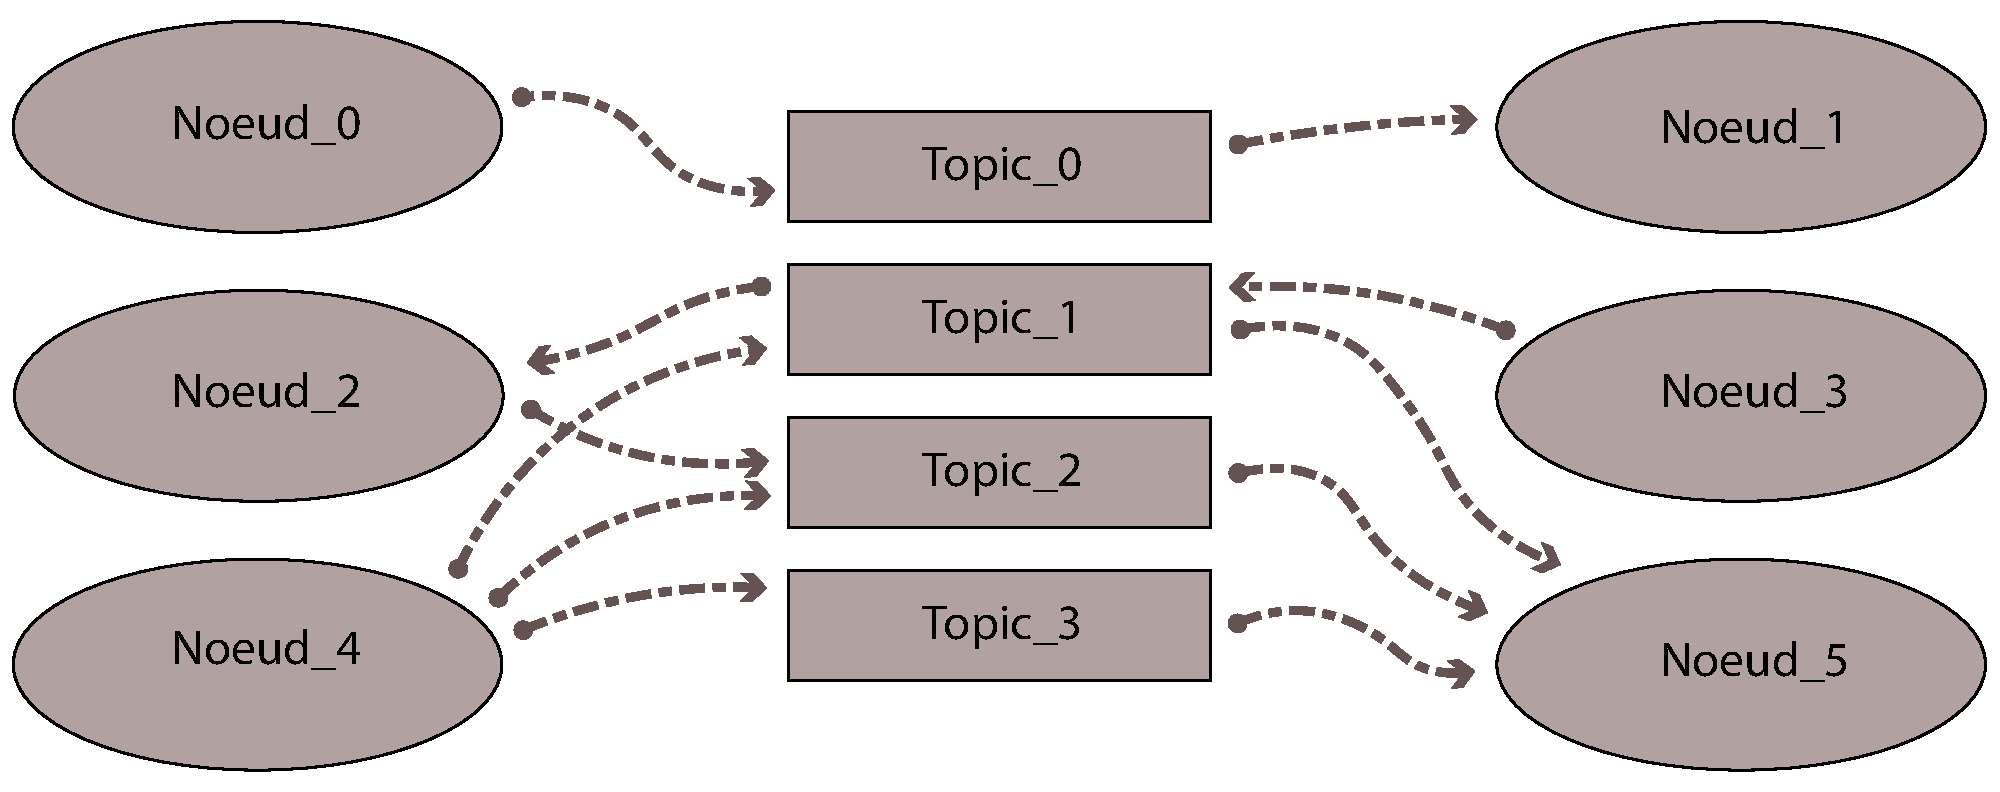
\includegraphics[width = 15cm]{figures/schema_topics_ros}
    \caption{Exemple d'utilisation des topics \gls{ROS}}
    \label{fig:topics}
\end{figure}
\subsubsection{Communication inter noeuds : les Services}
Les services permettent d'implémenter un mécanisme de communication Requête/Réponse, qui peut être utile dans un système distribué par exemple. Un service est défini par une paire de messages, un pour la requête et un pour la réponse. Un client envoie une requête et attend la réponse du noeud fournissant le service.


\section{Noeud Hexapod\_description}

\subsection{Fichier URDF}
Noeud Ros sert à la mise à jour et à la visualisation du fichier URDF\footnote{URDF est l'acronyme de Unified Robot Description File.} contenant le modèle du robot. Ce dernier permet de stocker de nombreuses informations dont :
\begin{itemize}
    \item les liens ou "links" : tout objet solide non animé.
    \item les articulations ou "joints" : liaisons entre les liens, dans notre cas les \gls{servomoteur}s principalement.
    \item les formes destinées à la génération du visuel de chaque lien.
    \item les formes destinées aux calculs de collisions de chaque lien.
    \item les positions de chaque articulation, cela nous sera utile pour calculer la cinématique du robot.
    \item les capteurs embarqués, ainsi que le nom du Topic sur lequel ils devront écrire.
    \item les poids et centre de gravité de chaque élément.
\end{itemize}

Cette liste n'est pas exhaustive, il est également possible de stocker des meshs et d'autres informations. Un exemple tiré d'une jambe de notre robot est disponible en annexe \ref{lst:exempleURDF}. Dans cet exemple, vous pouvez voir un joint et un link complets. 

C'est un format de fichier basé sur le standard XML\footnote{Standard XML : \url{https://www.w3.org/TR/xml/}}, il est donc lisible facilement avec n'importe quel éditeur de texte, et il permet également d'étendre les balises disponibles afin d'ajouter des données correspondant à une nouvelle fonctionnalité. 



Ce fichier de description du modèle de notre robot sera utilisé à la fois par le noeud ROS de simulation présenté en \ref{lb:rosdart} et par le contrôleur présenté en \ref{lb:controleur}.

\subsection{Génération par Macro}
\label{lb:xacroprez}
Comme vous avez pu le remarquer, stocker ne serait-ce qu'un link et un joint associé demande de nombreuses informations, et créer ce fichier à la main se révélerait long et fastidieux. Fort heureusement, les données du modèle comportent de nombreuses redondance. Il est possible de générer ce fichier de description URDF à l'aide d'un langage de macro appelé Xacro\footnote{Xacro pour XML macros : \url{http://wiki.ros.org/xacro}}. Nous l'utiliserons dans la partie \ref{lb:xacro}, ou seront présentés la syntaxe et le travail réalisé sur le modèle du robot.   

\newpage
\subsection{Visualisation du modèle}
Afin de valider le modèle du robot, il fallait un outil puissant capable à la fois de visualiser le modèle et de récupérer des données. Être capable enfin de changer les positions des \gls{servomoteur}s permet de récupérer les positions des extrémités des pattes du robot dans une position particulière, ce qui sera vraiment utile dans la partie de calcul de la cinématique du robot en \ref{lb:kinematics}.

Fort heureusement, ROS propose un outil adapté à ces besoins, nommé Rviz\footnote{Documentation disponible ici : \url{http://wiki.ros.org/rviz}}. Il a fallu mettre à jour le fichier de description afin d'y inclure des "transmissions" permettant de manipuler directement le modèle en lui envoyant des commandes de position pour chaque \gls{servomoteur}. Ces ajouts seront détaillés dans la section \ref{lb:xacro}.

\section{Noeud Hexapod\_bringup}
Ce noeud ROS permet de lancer l'interface matérielle avec les \gls{servomoteur}s. Il contient de nombreuses informations utiles comme les corrections d'angles de chaque \gls{servomoteur}, et permet également de lier les ids réels des moteurs avec des étiquettes, plus faciles à appréhender, permettant de savoir facilement à quel \gls{servomoteur} on envoie une commande. 

C'est un noeud qu'il convient de lancer avant chaque expérimentation sur le robot réel, il se contente d'attendre une commande de moteur sur un topic \gls{ROS} particulier. 

Seule la commande en position est possible, et la vitesse d'exécution de la commande est fixe, paramétrée à la vitesse angulaire maximale des servos-moteurs. Ceci a pour conséquence des mouvement pouvant être très brusques selon la différence entre la commande et le statut actuel. 

Le contrôleur \gls{ROS} utilisé par hexapod\_bringup permet de gérer des trajectoires, ensembles de commandes associées à un temps donné. Ce contrôleur permet également de récupérer une information quant au déroulement de la trajectoire, permettant ainsi de savoir par exemple si le point donné est erroné\footnote{Plusieurs causes possibles comme par exemple un point qui se situerait avant le temps présent.}, s'il a bien été atteint, ou s'il n'a pas pu être atteint à temps. Cette information peut se révéler extrêmement utile, notamment lors des phases de débuggage. 

\clearpage
\section{Noeud Optoforce}
Ce noeud permet de communiquer avec un capteur de force. Il lance l'interface matérielle permettant de récupérer la valeur étalonnée de la force appliquée sur le capteur. C'est un noeud ROS fourni par le vendeur des capteurs de force. 

Auparavant noeud indépendant qu'il fallait lancer pour chaque capteur de force, il a été modifié par Dorian Goep afin de l'intégrer dans Hexapod\_bringup, qui s'occupe désormais de tout préparer afin de pouvoir récupérer les valeurs sur des topics aux noms contenant l'identifiant du capteur, qu'il faudra par la suite lier à la patte correspondante. 

\section{Noeud Rosdart}\label{lb:rosdart}
Noeud permettant de simuler l'hexapode dans son environnement grâce à la librairie \gls{DART} tout en communiquant avec \gls{ROS} permettant ainsi de ne pas changer le code entre les tests en simulation et les tests réels. Le noeud Rosdart se substitue aux interfaces matérielles de manière totalement transparente. Ce noeud n'existait pas lors de mon arrivée dans l'équipe. Sa création a été plébiscitée par le besoin d'un simulateur générique pour les robots contrôlés avec \gls{ROS}. Nous pouvons en voir l'interface sur la figure \ref{fig:rosdartgui}.

Après avoir réalisé un prototype simple, un membre plus expérimenté de l'équipe, Konstantinos Chatzilygeroudis, a réalisé une version plus générique et plus puissante, permettant de gérer les capteurs de forces et de charger les contrôleurs directement depuis un fichier \gls{URDF} contenant la description du robot : ses liens, ses actionneurs, ses formes pour la visualisation, ses formes pour les collisions etc. C'est cette version qui sera utilisée durant le reste du stage.

\begin{figure}[h]
    \centering
    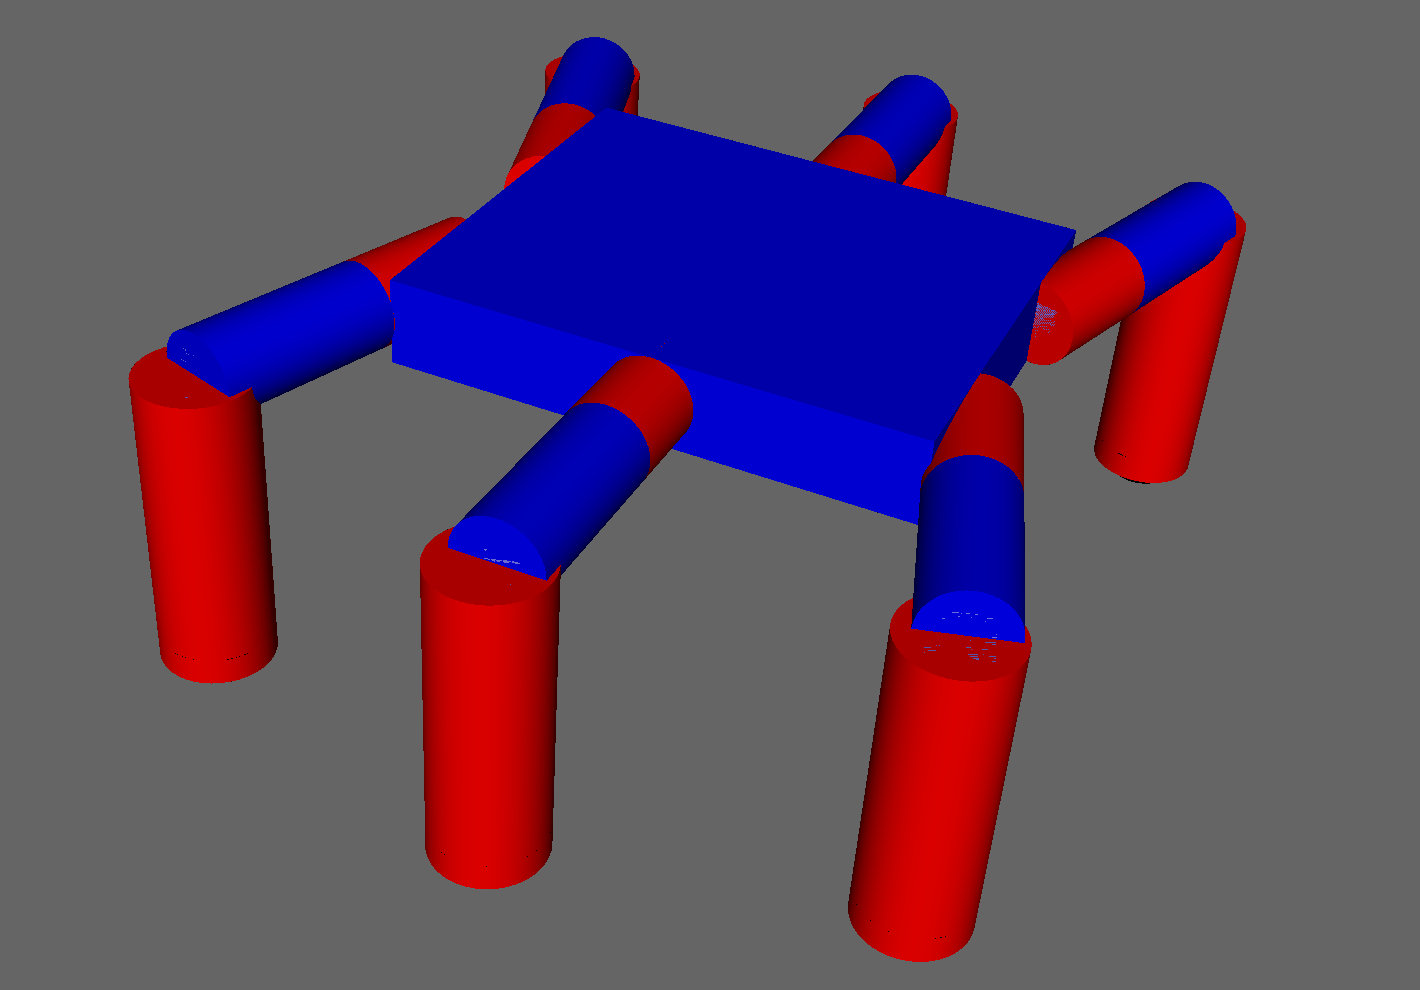
\includegraphics[width=8cm]{figures/rosdart}
    \caption{Capture d'écran de l'interface graphique de RosDart}
    \label{fig:rosdartgui}
\end{figure}

\section{Noeud Hexapod controler}\label{lb:controleur}
C'est le noeud destiné à contrôler le robot, qui devra envoyer des commandes aux moteurs en fonction des capteurs du robot et des entrées de plus haut niveau comme des commandes de direction, de vitesse ou de position. C'est l'objectif de ce stage, ce noeud sera réalisé entièrement lors de celui ci, il constituera donc le principal travail effectué et sera détaillé dans le chapitre \ref{lb:travail}.



\chapter{Contribution}\label{lb:travail}
Les bases permettant une bonne compréhension du système et du projet ayant été présentées, nous pouvons maintenant aborder le coeur des travaux réalisés dans le cadre de ce stage. 

L'idée ici est de présenter les phases de conceptions des différentes composante du système, les problèmes rencontrés, les méthodes utilisées pour les identifier ainsi que les solutions mises en place pour pallier à ces imprévus. 

\section{Principes de base}
Le contrôleur se basera principalement sur différents concepts tirés des approches pragmatiques présentées en \ref{lb:pratique}. Comme évoqué auparavant, les approches biomimétiques, bien qu'intéressantes, se révèlent peu documentées, et certainement trop complexes pour l'objectif à réaliser. 

Combiner différentes approches de différents niveaux, basées sur des concepts pratiques et connus, devrait permettre d'atteindre l'objectif fixé dans le temps imparti. 

Une mécanique de modules découplés sera également mise en place afin de rendre l'ensemble polyvalent.

Afin de simplifier la compréhension des mécanismes du contrôleur, nous nous référerons à la figure \ref{fig:schemectrl} dans cette section. 
\subsection{Les entrées du système}
L'idée d'un contrôleur omnidirectionnel ayant séduit l'équipe resibots, ce dernier devra être capable de prendre en commande un vecteur de déplacement ainsi qu'une fréquence de déplacement\footnote{Ici la fréquence de déplacement correspond au nombre de pas effectués par secondes.}. 

Les codeurs de positions intégrés aux servomoteurs seront pris en compte par le système, notamment pour la génération de la trajectoire des pattes. 

Les capteurs de forces situés à l'extrémité de chaque pattes doivent également êtres pris en comptes afin d'adapter le comportement au terrain et ainsi le rendre plus robuste aux terrains difficiles.
\subsection{Module de synchronisation : Hexapod}
Comme vu précédemment dans de nombreuses publications issus à la fois de la biomimétique et des approches plus pragmatiques, il est bon d'avoir des pattes indépendantes afin de pouvoir découpler la synchronisation de la génération de trajectoires de chaque patte. 

Nous aurons donc un bloc fonctionnel \textit{Hexapod} chargé de la création des pattes, puis de la synchronisation de ses dernières en fonction de la fréquence de commande globale. Cela permet notamment de travailler avec un nombre variable de pattes, ce qui est utile dans notre cas pour simuler par exemple la perte d'une patte. L'autre avantage de ce découplage et qu'il permet de changer facilement le mécanisme de synchronisation des pattes pour implémenter une autre approche si cela s'avère nécessaire. 
Le bloc \textit{Hexapod} à également pour rôle de récupérer les positions des servomoteurs et les valeurs des capteurs de force puis de les propager aux pattes concernées par ses informations. L'intérêt de récupérer ses valeurs ici et non directement dans les pattes est de pouvoir, si le temps nous le permet d'implémenter par la suite des algorithmes de type \gls{MPC}. Ces informations seront en effet nécessaire à l'établissement d'un modèle du robot ou encore d'une carte des forces appliquées sur ce dernier.   

\subsection{Des pattes indépendantes}
Enfin, pour compléter les rouages du mécanisme, les pattes jouent un rôle important. Étant indépendantes, elles comportent chacune une génération de trajectoires, un module de calcul de cinématique et un module de communication.
\subsubsection{Module de génération de trajectoires}
En effet, pour simplifier et surtout mieux maîtriser les trajectoires réalisées par les pattes, la génération de ces mêmes trajectoires se fera en coordonnées cartésiennes, et non dans l'espace de position des servomoteurs. Cela présente de nombreux avantages, le principal étant que raisonner en cartésien est plus naturel pour nous, nous permettant de déplacer la patte exactement comme on le souhaite. La génération des trajectoires sera présentée en \ref{lb:trajectory}. 
\subsubsection{Module de calculs cinématiques}
On l'a vu, il est plus intéressant de générer les trajectoires en coordonnées cartésiennes. Seulement les moteurs, eux, doivent êtres commandés en positions angulaires. Il faut donc une connexion à double sens permettant de passer aisément d'un domaine à l'autre. C'est le module de calculs cinématiques présenté en \ref{lb:kinematics}, second élément composant chaque patte.
\newpage
\subsubsection{Module de communication avec les servomoteurs}
Enfin il est nécessaire de communiquer les trajectoires crées puis traduites en ordres aux servomoteurs. C'est le rôle du module de communication. Son rôle est assez explicite, et son fonctionnement sera présenté en \ref{lb:communication}.

Ces élément, une fois réalisés et interconnectés, permettront à notre contrôleur de remplir les objectifs qui lui sont fixés. Rappelons : un nombre de paramètres d'entrée faible, une mobilité omnidirectionnelle, et enfin une prise en compte des capteurs de force afin de permettre une réactivité vis à vis du terrain. 
\begin{figure}
    \centering
    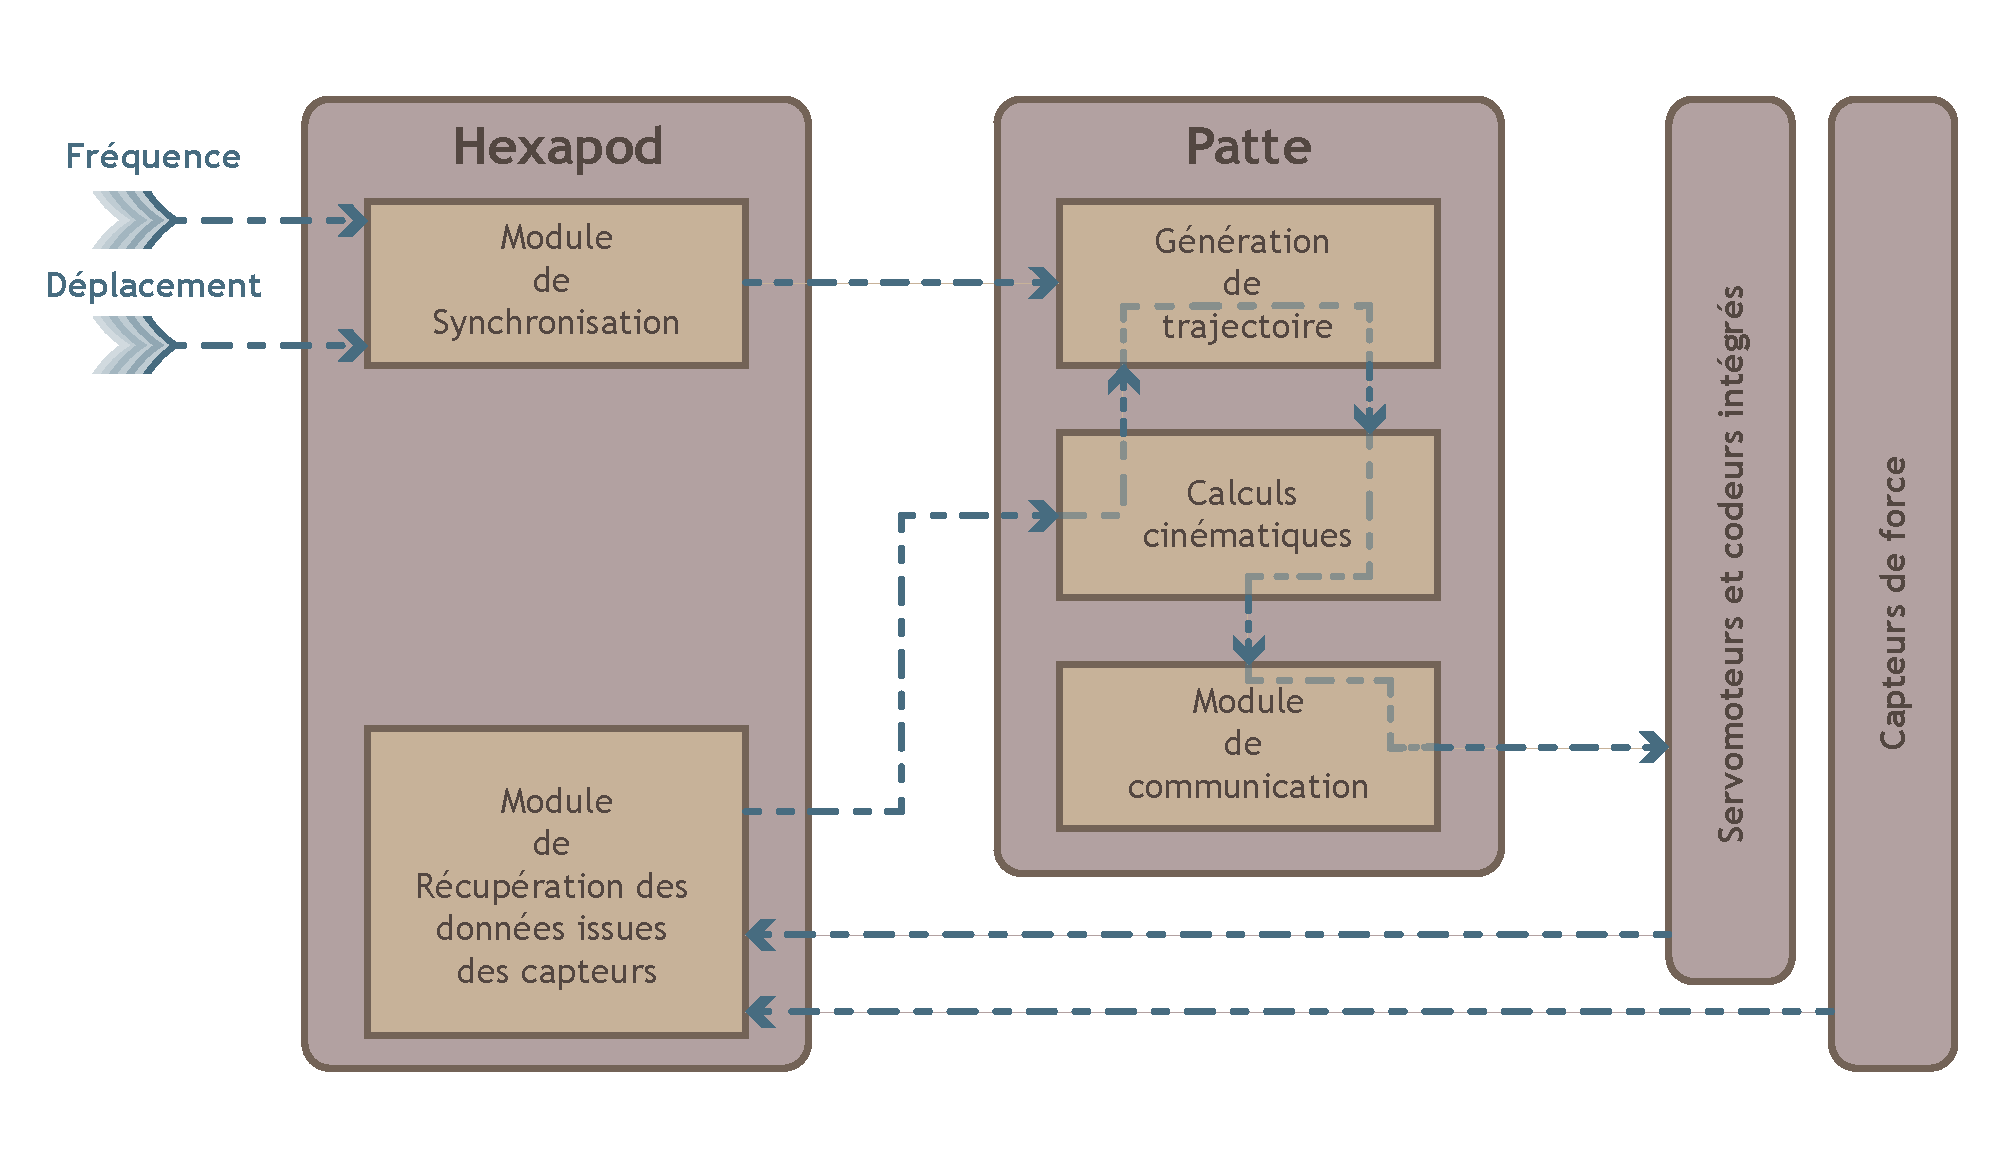
\includegraphics[width=17cm,angle=-90]{figures/concept}
    \caption{Schéma global du contrôleur}
    \label{fig:schemectrl}
\end{figure}
\clearpage

\section{Méthodes}
La recherche impose une méthode particulière. L'incertitude quant aux résultats que produira une solution ainsi que le manque occasionnel d'informations sur l'implémentation de cette dernière peuvent conduire à une importante perte de temps. En effet, il est possible qu'en raison du manque de documentation, du manque de mise à jour d'une librairie, une solution autrefois fonctionnelle ne le soit plus, demande beaucoup de temps pour adapter son code aux éventuels changements d'API ou encore les deux. Nous en verrons deux exemples concrets dans la section \ref{lb:kinematics}. 

Afin d'éviter de perdre trop de temps en essayant d'implémenter proprement une fonctionnalité issue d'une librairie/solutions incertaine, il convient de travailler au plus rapide, afin d'arriver à un résultat, positif ou non, dans les plus bref délais. 

De prime abord confiant dans l'apparente simplicité de la tâche à réaliser, j'ai commencé par réfléchir aux bonnes façon de procéder, d'emblée prêté attention à l'optimisation, porté au final beaucoup d'attention mais surtout de temps dans la réalisation et le développement d'une solution, avant même d'avoir la certitude que cela allait fonctionner. 

C'est un revers qui m'a permis d'en tirer une leçon, et de mettre à jour ma façon de procéder pour la suite du stage, me permettant par la suite un gain de temps non négligeable. 

La méthode émergeant de ce problème est de réaliser un prototypage rapide afin de s'assurer rapidement de la validité pratique de la solution essayée.

\subsection{Gestionnaire de versions}

L'équipe utilise deux serveurs Git, l'un accessible à tous sur github\footnote{L'adresse est la suivante : \url{https://github.com/resibots/}} qui comprend donc les travaux suffisamment aboutis et non confidentiels pour être publiés librement. Elle contient donc le dépôt \textit{hexapod\_ros} contenant les noeuds \textit{hexapod\_description} et \textit{hexapod\_bringup}.

L'autre est un serveur interne au \gls{LORIA}. Il nécessite une connexion locale ou le recours à un \gls{VPN} afin d'y accéder. Il comporte quant à lui les travaux expérimentaux et/ou pas assez développés à l'heure actuelle. C'est là qu'est sauvegardé le noeud réalisé pendant ce stage (\textit{hexapod\_controller}) ainsi que le noeud \textit{rosdart}. 

\subsection{Prototypage}
Après les premiers écueils, le prototypage s'est rapidement imposé comme une évidence afin de sauvegarder du temps. L'idée est relativement simple, il s'agit ici de chercher à converger rapidement vers des résultats, afin d'identifier le potentiel d'une librairie. Il est en effet inutile de consacrer trop de temps à l'implémentation propre et commentée d'une solution si celle-ci s'avère inefficace ou pire inappropriée. 

\subsubsection{Réalisation du prototype}
Le prototype est découplé du code existant, il est indépendant et testé sur un exemple similaire permettant toutefois de valider ou non sa pertinence. Ne pas l'intégrer au reste du code directement permet d'éviter de prendre du temps dans une architecture compliquée. L'idée est ici de "simuler" le contexte d'exécution désiré, d'effectuer un test puis de comparer avec les résultats attendus. 

Ce découplage permet également d'ignorer dans un premier temps les éventuels problèmes de dépendance de librairies ou de compatibilité avec ROS. Ces problèmes sont bien évidement contournables, mais l'idée ici reste de gagner du temps. 

\subsection{Intégration}
Une fois une solution validée par un prototype, il convient de l'intégrer dans l'architecture existante, afin d'en valider la pertinence réelle. On est alors confrontés à différents problèmes d'intégration dans ROS, ou encore d'incompatibilité en l'état avec l'architecture.

\subsubsection{Adaptation de la solution}
De nombreux changement sont parfois à prévoir en passant d'un prototype codé rapidement et indépendamment à une implémentation plus propre et complexe au sein de l'architecture de notre contrôleur. Ce fut principalement le cas pour les solutions de calculs cinématiques vues en \ref{lb:kinematics}. La souplesse d'utilisation des librairies étant fortement variables, les adaptations nécessaires dépendent beaucoup de la solution, et peuvent nécessiter de faibles changements comme la réécriture d'une partie de la librairie.    

\subsection{Tests en Simulation}
En plus d'une validation numérique chiffrée du comportement obtenu à partir d'une solution, il est important de valider le comportement du robot exploitant cette solution. Toutefois, dans le but de préserver le robot de comportement destructeurs du à des erreurs de calculs d'une solution inadaptée, il est conseillé de simuler l'expérience dans un premier temps. 

Lors de ces test il est également bon d'enregistrer des données comme les trajectoires générées, afin de pouvoir vérifier de manière précise que l'on a atteint le comportement initialement désiré. De plus, de nombreuses données ont parfois des influences trop minimes pour êtres répercutées de manière visible lors d'une marche rapide du robot. 

Il est par la suite possible d'étudier ces données via ROSBAG par exemple qui permet d'enregistrer et de rejouer un scénario entier, comprenant tous les messages échangés sur les topics ROS. 

Il est également possible de visualiser les données sur un graphe, en utilisant par exemple l'outil matplotlib\footnote{matplotlib est une librairie open-source créée par John Hunter, elle permet la visualisation de données à travers de nombreuses figures différentes, comme des graphes, diagrammes, histogrammes etc...}

\subsection{Tests Réels}

Une fois le comportement validé en simulation (le comportement parait bon, il n'y a pas d'auto-collisions\footnote{Dans notre cas, une auto-collision peut survenir quand deux pas adjacentes reçoivent des commandes les rapprochant. Des valeurs limites de positions des moteurs sont définies, mais elle ne sont pas suffisamment restrictives pour éviter l'auto-collision dans un cas défavorable.}, pas de comportement destructif) il est important de tester le contrôleur sur le robot réel. 

En effet, de nombreux paramètres ne sont pas pris en comptes dans la simulation et d'autres divergent de la réalité. Comme par exemple la non-perfection des servomoteurs qui n'est pas prise en compte dans la simulation. Autre différence, les ressorts ne sont pas modélisés en simulation, ne permettant pas d'identifier d'éventuels problèmes de forces. Encore un point, et non des moindres, les servomoteurs sont considérés parfaits en simulation, et même si les modèles installés sur le robot sont de bonne qualité, il ne peuvent jamais atteindre exactement la commande demandée. 

Pour ces raisons, il s'avère nécessaire de tester le comportement directement sur le robot, dans des conditions réelles d'utilisation. Cela n'empêche pas, au contraire de continuer d'enregistrer des données en vue de leur éventuelle étude ultérieure en cas de défauts apparents. 

\section{Assemblage du robot}\label{lb:assemblage}
\subsection{Existant}
Le design des pattes avait déjà été réalisé lors de mon arrivée, les servomoteurs étaient déjà arrivés, les pièces imprimées en 3D l'étaient également. Le corps du robot, fait d'une plaque de circuit imprimé était déjà découpé. Il restait juste à agencer l'intérieur du robot pour y ajouter les circuits de traitement des capteurs de forces, de l'IMU ainsi que les hubs \gls{USB} et les hubs de puissance. 

\subsection{Mise en oeuvre des servomoteurs}
Les servomoteurs sont paramétrables, et ont par défaut un identifiant égal à 1. Il est indispensable de les changer, il n'est pas possible de les distinguer et donc de leur envoyer des commandes différentes. Un utilitaire développé par l'équipe \textit{libdynamixel}\footnote{C'est une librairie prenant en charge les servomoteurs permettant de communiquer simplement avec eux via une interface en ligne de commande et proposant une interface c++. Elle est disponible sur le github de l'équipe : \url{https://github.com/resibots/libdynamixel}} permet d'effectuer se changement d'identifiant par simple ligne de commande (qui ne sera pas détaillée ici car elle est encore sujet à changements). Il est néanmoins nécessaire de connecter les servomoteurs un à un. Afin de simplifier l'entretien du robot lors d'un éventuel démontage, chaque servomoteur a été étiqueté avec son identifiant. C'est une opération assez simple mais chronophage. 

Après avoir changé les identifiants, il convient de changer la vitesse de communication des servomoteurs. En effet, sa vitesse par défaut n'est pas au maximum de ses capacités, ce qui réduit la fréquence maximale de contrôle possible. La capacité du bus USB étant suffisante pour les 18 servomoteurs réglés au maximum, ce maximum de 1 000 000 de bauds a été choisi.

Cette opération est réalisable en broadcast, en une seule ligne de commande, permettant de changer cette vitesse sur tous les servomoteurs. 

\subsection{Organisation interne}
Avec l'ajout des capteurs de force et d'une centrale inertielles, les contraintes de place à l'intérieur du corps du robot sont devenues importantes. Il a donc fallu réfléchir à une organisation permettant de tout intégrer dans le corps du robot, tout en étant capable de retirer facilement les cartes de traitement des capteurs de force. Le design retenu est visible sur la figure \ref{fig:layout}. Nous pouvons y voir les servomoteurs des hanches aux extrémités de la carcasse, la centrale inertielle au milieu et les hubs/racks USB pour les capteurs de force. Viendront s'ajouter par la suite les circuits de puissance. et le connecteur USB extérieur.  

\begin{figure}
    \centering
    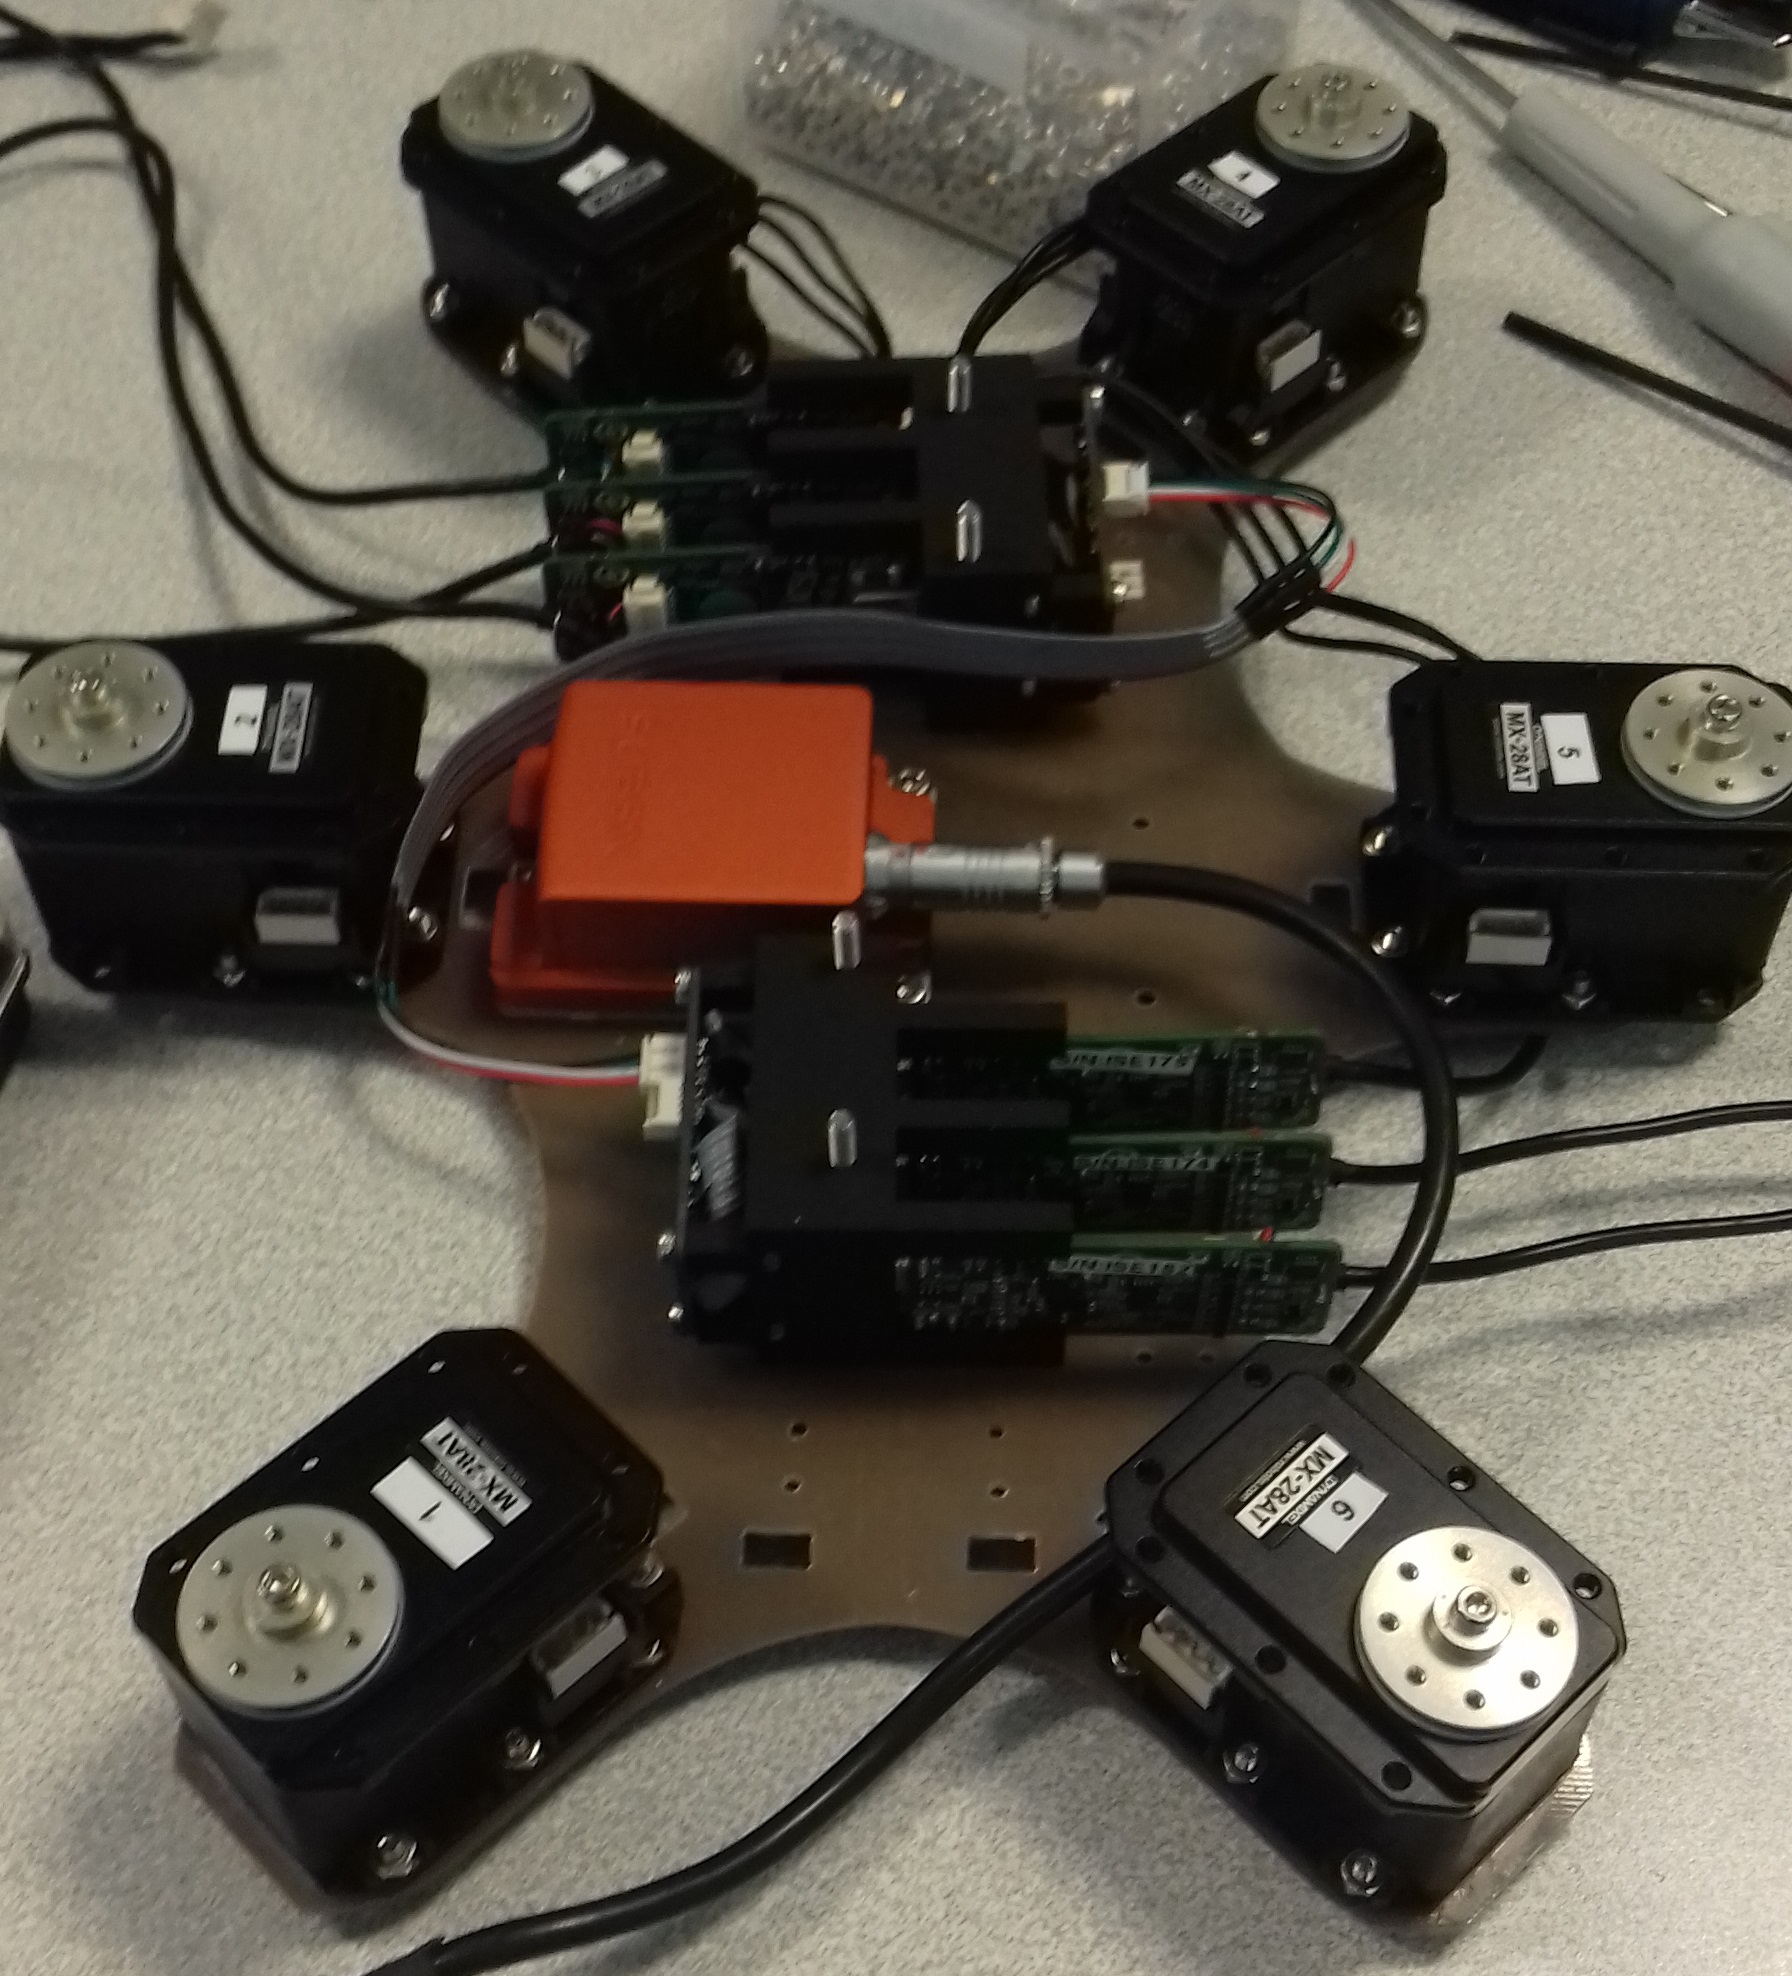
\includegraphics[width=10cm]{figures/layout}
    \caption{Organisation interne de l'hexapod}
    \label{fig:layout}
\end{figure}

\subsection{Mise on oeuvre des capteurs de force}
Afin d'intégrer les capteurs de force dans le boîtier, il a fallu sortir les cartes de traitement de leur protection initiale en aluminium, afin de pouvoir les intégrer dans un rack spécialement conçu pour l'occasion par Dorian Goepp. Il a également fallu souder des connecteurs aux hubs USB afin de pouvoir réaliser la connexion par la suite. 
\subsection{Problèmes de hubs USB}
L'alimentation par USB était trop peu puissante pour alimenter en simultané tous les capteurs de forces connectés. Il a donc été nécessaire d'ajouter une alimentation externe afin d'alimenter en conséquence les hubs USB. Cette alimentation externe est un régulateur de tension connecté sur le circuit d'alimentation des servomoteurs.

\section{Réalisation du bloc patte}
Nous aborderons ici la réalisation bloc fonctionnel indépendant d'une patte et des modules qui le composent. 

\subsection{Module de génération de trajectoires}\label{lb:trajectory}

Le mode de déplacement d'un robot/animal qui comporte des pattes peut se décomposer en deux phases à exécuter pour chacune de ses pattes, indépendamment du nombre de pattes ou de leur géométrie.

Dans le but de simplifier la compréhension du mécanisme, nous pouvons donc analyser notre propre façon de marcher. Chacune de nos jambes, passent tour à tour d'une phase de support, ou notre pied est en contact avec le sol et supporte notre poids, tout en nous propulsant dans la direction du mouvement de notre corps, à une phase de "swing" ou nous levons le pied afin d'atteindre la prochaine position d'appui. 

Il suffit alors de bien synchroniser les jambes afin de garder l'équilibre pendant la marche.  
\subsubsection{Utilisation du patron de conception Stratégie }
Comme vu précédemment, chacune des pattes de notre hexapode devra être capable d'effectuer différents types de mouvements, en fonction de la phase dans laquelle elle se trouve. 

Dans un premier temps, seuls deux phases : support et swing seront utilisées. Mais dans l'avenir, on peut facilement imaginer qu'il sera nécessaire d'implémenter d'autres phases, comme par exemple comme la procédure de réaction à un contact prématuré (un obstacle) détecté à l'extrémité d'une patte.

Dans le but de pouvoir changer dynamiquement pendant l'exécution du programme l'algorithme de génération de trajectoire d'une patte, nous emploierons un patron de conception nommé Strategy pattern.

Comme l'illustre la figure \ref{fig:strategy}, son principe est simple. Chaque objet de type patte se voit assigner une stratégie implémentant l'interface Strategy, offrant une fonction de génération de trajectoire ainsi qu'une fonction de vérification de la force appliquée sur le capteur de force. 

\begin{figure}[h]
    \centering
    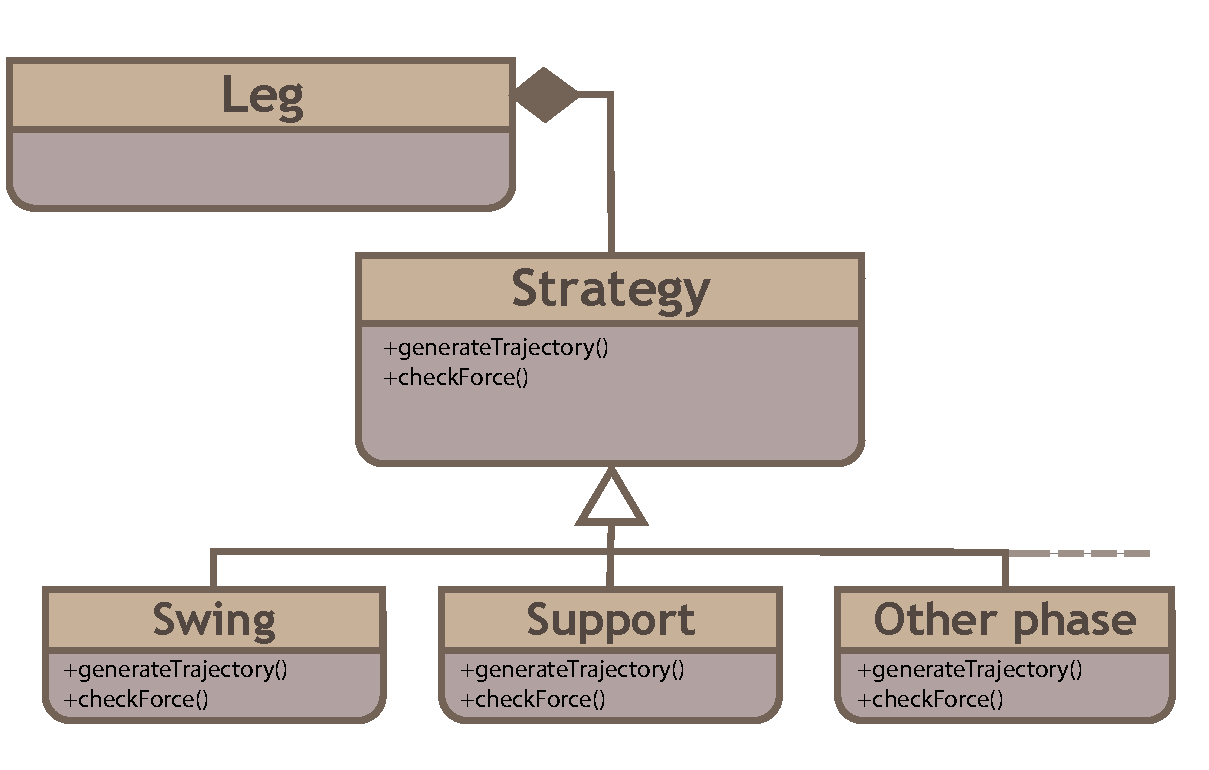
\includegraphics[width = 14cm]{figures/strategy}
    \caption{Schéma UML de l'implémentation du pattern Strategy}
    \label{fig:strategy}
    
\end{figure}
Le changement de stratégie s'effectue soit lorsque l'un nouveau cycle commence, soit sur la base de la vérification de force. Notamment lorsque l'on touche un obstacle avant la fin programmée de la trajectoire. 

L'avantage de ce mécanisme réside entre autres dans le découplement opéré entre la synchronisation globale et dans la réalisation des trajectoires. 

\subsubsection{Support}
La patte en phase de support doit non seulement porter le robot, mais également permettre au corps du robot de suivre le mouvement des pattes qui sont en  phase swing afin de le faire avancer. Il faut donc que le point de contact avec le sol reste fixe tandis que le corps du robot doit suivre la direction du mouvement. 

Le principal problème ici est que l'on commande en position l'extrémité de la patte du robot et non le corps directement. L'astuce illustrée par la figure \ref{fig:supporta} est la suivante : afin d'effectuer le vecteur de déplacement souhaité (ici représenté en bleu) on utilisera le contact avec le sol. En maintenant ce contact avec le sol, et en comptant sur un minimum d'adhérence de la surface de contact, on fixe l'extrémité de la patte, qui permettra à la patte de déplacer le corps du robot d'un vecteur inverse du vecteur de commande bleu. 

Il suffit alors d'inverser ce vecteur de commande ce qui donne le vecteur représenté ici en vert, afin d'obtenir le comportement désiré. Il suffit par la suite de calculer, a partir de la position actuelle qui peut être calculée\footnote{Grâce à la cinématique directe} à partir des positions des servomoteurs données par les codeur de position. On ajoute par la suite le l'inverse du vecteur de commande à cette position pour trouver la position, à atteindre à la fin de la trajectoire. 

\begin{figure}[h]
\centering
\subfloat[Vecteur de déplacement à effectuer]{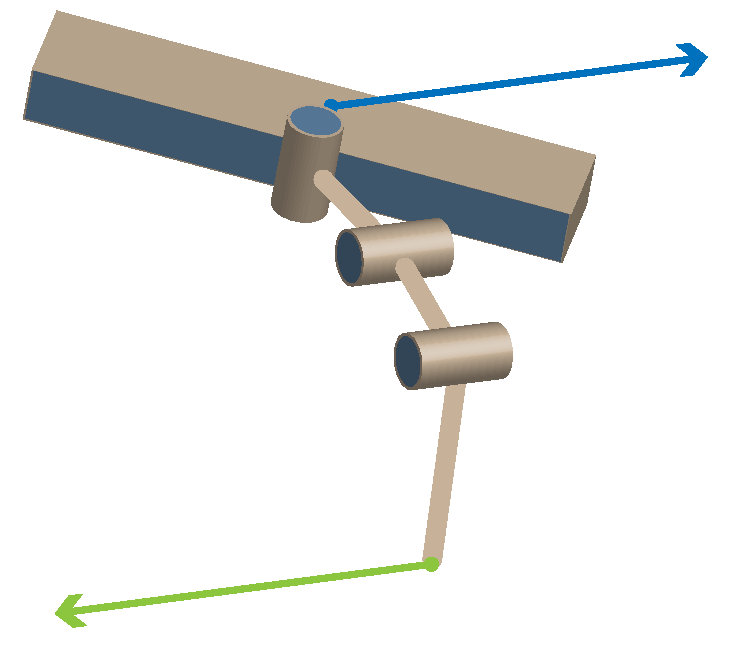
\includegraphics[width = 7.5cm]{figures/support-base}\label{fig:supporta}}\qquad
\subfloat[Trajectoire générée]{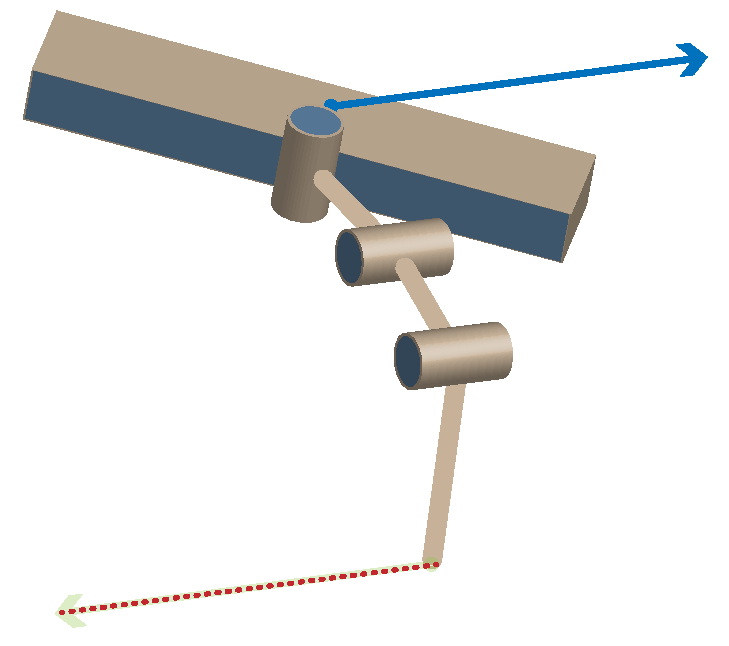
\includegraphics[width = 7.5cm]{figures/support}\label{fig:supportb}}\\
\caption{Schéma de la génération de trajectoire support}
\label{fig:support}
\end{figure}
Une fois l'origine et la destination de la trajectoire connue, il suffit de générer des points en $n$ étapes, en ajoutant à chaque fois une fraction du vecteur de commande correspondant à :
\begin{equation}
objectif = position + \frac{commande}{n}
\end{equation}
 avec $objectif$ qui correspond à la position à atteindre à la fin de l'étape, $position$ qui correspond à la position de l'étape précédente, ou de la position actuelle de la patte dans le cas de la première itération.

Puis on répète cette opération $n$ fois, afin de générer tous les points de la trajectoire représentés dans la figure \ref{fig:supportb} par les points rouges le long du vecteur vert. 

Plus le nombre d'itérations $n$ est grand, plus la trajectoire sera précise. En effet, comme l'on peut le voir sur la figure \ref{fig:traj} si l'on donne directement la dernière position aux servomoteurs, il vont tenter de l'atteindre le plus vite possible. Sans forcément suivre une trajectoire rectiligne (ici une trajectoire probable est représentée en pointillés rouges. Comme vous pouvez le voir la trajectoire réelle empruntée par la patte dans ce cas est loin d'être rectiligne, ce qui peut provoquer des glissements lorsque plusieurs pattes d'un côté opposé effectuent leur phase de support. C'est pour cette raison que l'on crée une trajectoire avec plusieurs points intermédiaires, permettant de lisser la trajectoire réelle de la patte. 

\begin{figure}[h]
\centering
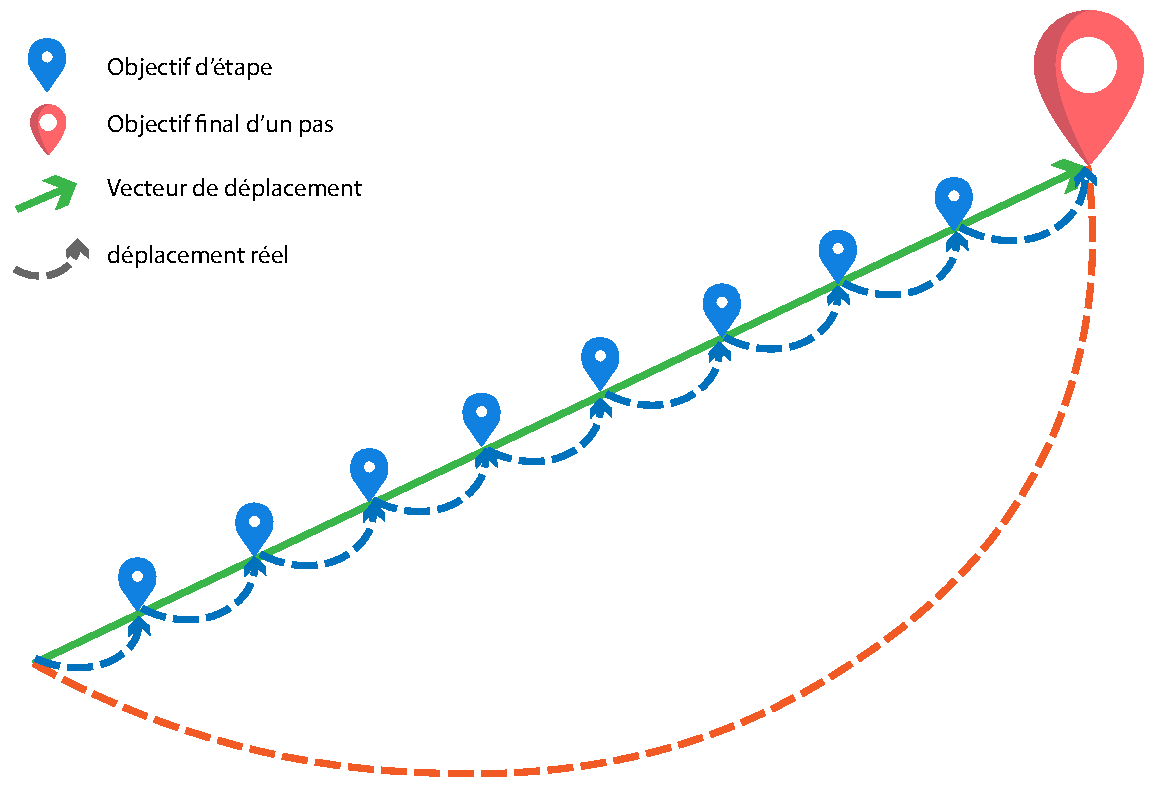
\includegraphics[width = 15cm]{figures/traj}
\caption{Lissage de la trajectoire}
\label{fig:traj}
\end{figure}
En pratique, il a été déterminé empiriquement que $n=100$ était un bon compromis entre temps de calcul nécessaire et précision de la trajectoire. En effet, même si une simple suite de divisions puis d'additions n'est pas très gourmande en puissance de calculs, le passage du domaine cartésien aux commandes de moteurs est quant à elle plus exigeante comme nous le verrons dans la partie \ref{lb:kinematics}. Il convient donc de limiter le nombre de points générés afin de pouvoir travailler en temps réel. 

\subsubsection{Swing}

Concernant la phase de swing, l'objectif est de faire avancer la patte du vecteur de commande. Pour $x$ et $y$, il suffit alors de suivre ce vecteur. En revanche, il faut lever la patte afin d'éviter les frottements avec le sol. La composante $z$ est alors augmentée progressivement jusqu'à atteindre le milieu de la trajectoire, puis diminuée jusqu'à atteindre la même valeur qu'au début de la phase de swing. La figure \ref{fig:swing} illustre ces propos. Vous pouvez voir que pour pouvoir continuer le mouvement selon le vecteur de commande (ici en bleu), il faut déplacer la patte de ce même vecteur, on calcule donc l'objectif du pas en additionnant le vecteur à la position courante de l'extrémité de la patte, ce qui représente le vecteur de déplacement vert. La trajectoire ici générée est représentée en rouge.

\begin{figure}[h]
\centering
\subfloat[Vecteur de déplacement à effectuer]{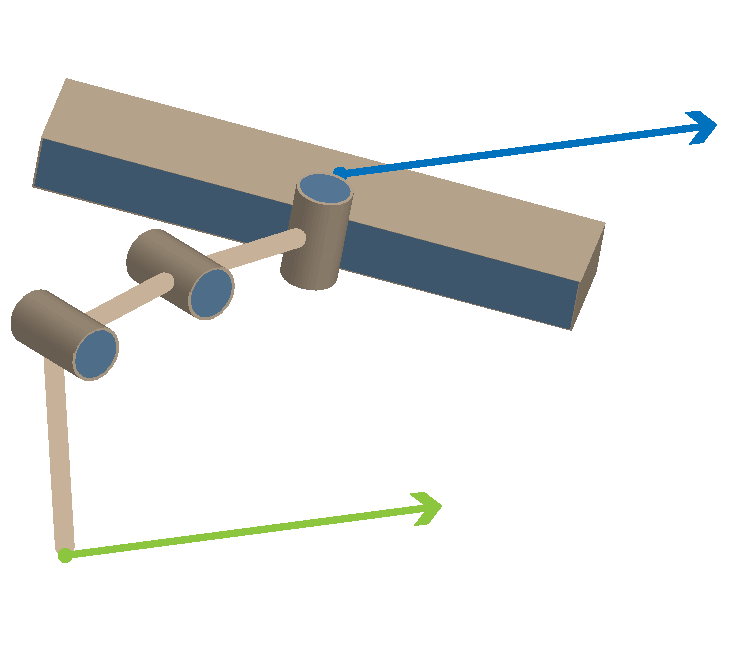
\includegraphics[width = 7.5cm]{figures/swing-base}}\qquad
\subfloat[Trajectoire générée]{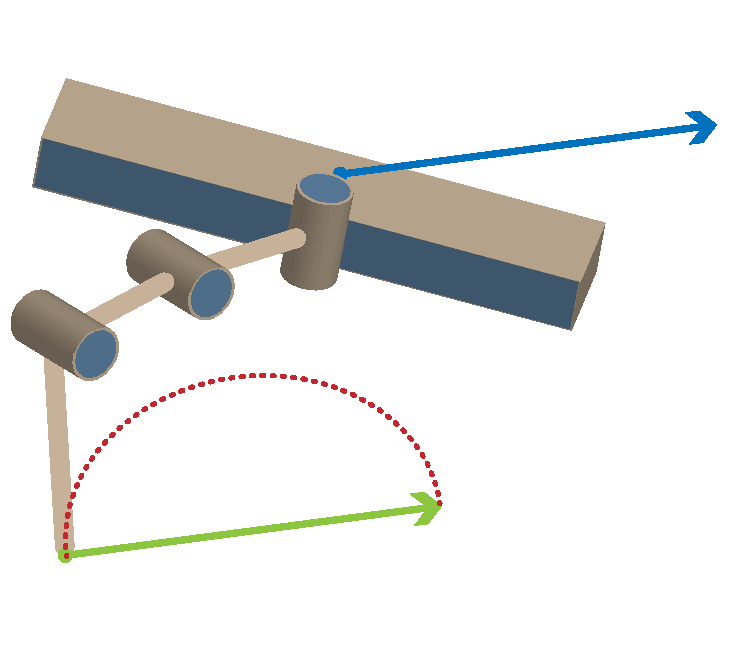
\includegraphics[width = 7.5cm]{figures/swing}}\\
\caption{Schéma de la génération de trajectoire swing}
\label{fig:swing}
\end{figure}

La trajectoire en triangle ainsi générée avait l'inconvénient de faire glisser l'extrémité de la patte sur le sol, ce qui a pour conséquence de ne pas totalement respecter le vecteur de déplacement commandé. Il faut donc trouver une alternative, afin de générer une trajectoire plus adaptée sur l'axe $z$.

Il existe de nombreuses possibilités pour générer une trajectoire en deux dimensions sont infinies. Mais de quoi avons nous besoin ? Ces quelques critères on permis de choisir une courbe plus adaptée : 
Il fallait que la trajectoire soit perpendiculaire au sol lors du contact, afin de mieux adhérer et ainsi éviter les glissement. Il fallait également que la patte se lève rapidement afin d'éviter naturellement de nombreux obstacles de petites dimensions qu'il aurait fallu gérer autrement. Enfin il fallait que le calcul soit simple et que l'équation de la courbe soit hautement paramétrable. 

Après quelques recherches, il semblait qu'une demi-ellipse soit adaptée à nos besoins en répondant à tous nos critères. 

L'équation de la Courbe est la suivante :

\begin{equation}
   zEtape = zMax * \sqrt{1 - \frac{k}{0.5 - 1} * \frac{k}{ 0.5 - 1}}
\end{equation}

Ici $zMax$ permet de déterminer la hauteur maximale de la courbe et ainsi d'ajuster la hauteur de la patte selon nos besoins. $k$ correspond ici au temps de l'étape. la figure \ref{fig:trajplot} montre les courbes $x$ (en bleu), $y$ en vert, et $z$ en rouge, qui correspond à l'ellipse décrite ci-dessus. 
\begin{figure}[h]
    \centering
    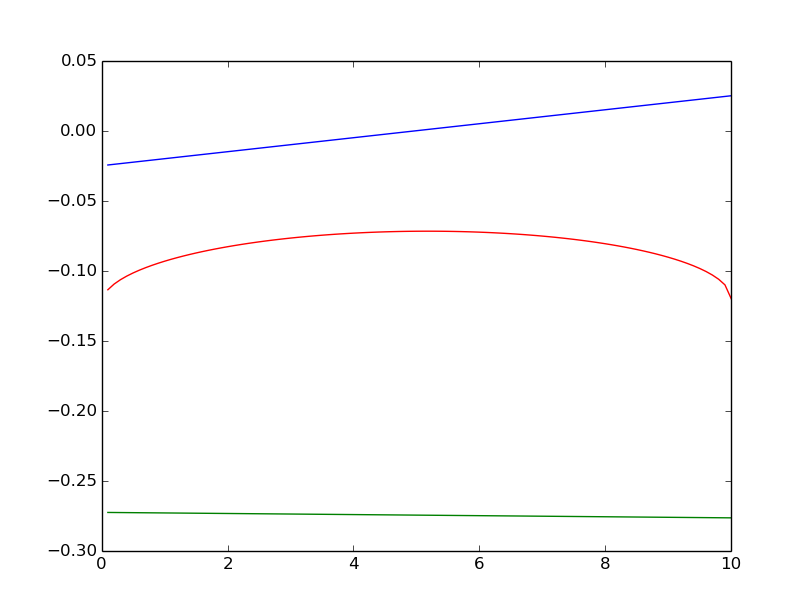
\includegraphics[width=8cm]{figures/beforeIK}
    \caption{Trajectoire elliptique générée}
    \label{fig:trajplot}
\end{figure}

\subsubsection{Correction du vecteur de déplacement}\label{lb:corrvect}
Après avoir implémenté et testé ces deux phases, il s'est avéré que les perturbations étaient conservées dans le temps, menant à une dérive. C'est logique car la position à atteindre est calculée à partir de la position actuelle, qui n'est pas exactement la position commandée à cause des perturbations extérieures comme la gravité.

Il faut alors trouver une solution afin de calculer le point objectif de manière absolue afin de compenser cette dérive quelques soient les perturbations extérieures. L'idée retenue, illustrée sur la figure \ref{fig:comp} est de calculer l'objectif à atteindre à partir d'un point fixe dans l'espace. 

Le choix le plus simple et logique était d'utiliser le point neutre de chaque patte, correspondant à la position cartésienne de l'extrémité de la patte lorsque les servomoteurs sont à leur position initiale. Ce point se calcule facilement grâce au module de cinématique directe présenté en \ref{lb:kinematics}. Une fois cette position déterminée, il suffit de lui ajouter la moitié du vecteur de commande afin de trouver la position à atteindre à la fin du pas. 

\begin{figure}[h]
\centering
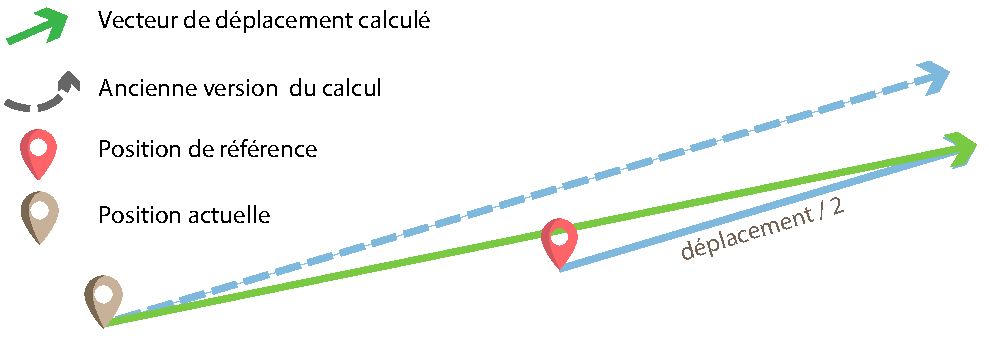
\includegraphics[width = 13cm]{figures/correctionprinc}
\caption{Principe de la correction du vecteur de déplacement}
\label{fig:comp}
\end{figure}

Utiliser cette astuce permet donc de compenser les dérives dans le temps, mais n'évite pas les erreurs dues au correcteur intégré des servomoteurs. La figure \ref{fig:corr} illustre la dérive de l'ancienne version et la façon de compenser décrite précédemment. On constate bien qu'il y a toujours une inévitable erreur, mais celle ci est minime, et surtout elle ne se cumule pas. Cette erreur est donc rendue négligeable par la compensation.   

\begin{figure}[h]
\centering
\subfloat[calcul relatif]{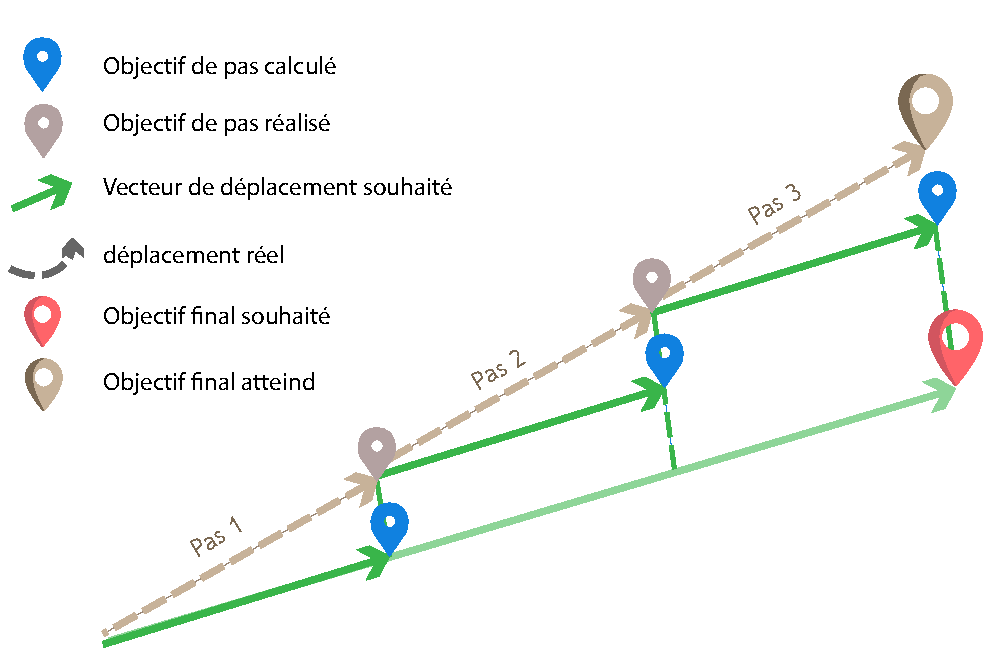
\includegraphics[width = 7.5cm]{figures/correction}}\qquad
\subfloat[calcul absolu]{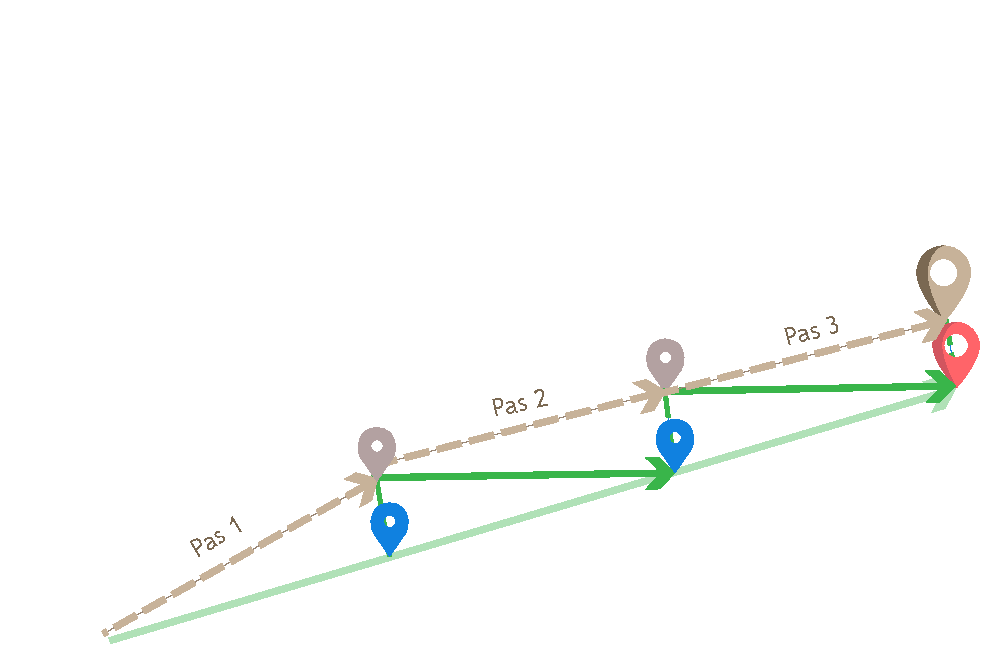
\includegraphics[width = 7.5cm]{figures/correction2}}\\
\caption{Effets de la compensation par calcul absolu de l'objectif}
\label{fig:corr}
\end{figure}

\newpage
\subsection{Module de calculs cinématiques}\label{lb:kinematics}
Ce module à pour objectif de passer du repère cartésien au repère de commande des servomoteurs. le repère cartésien est représenté par un vecteur de coordonnées : 
\begin{equation}
cart= 
    \begin{pmatrix}
    x \\
    y \\
    z \\
\end{pmatrix}
\end{equation}

Tandis que le repére de commande est composé de trois angles en radians :
\begin{equation}
    jnt= 
    \begin{pmatrix}
    \theta_1 \\
    \theta_2 \\
    \theta_3 \\
\end{pmatrix}
\end{equation}

Différentes solutions ont été testées lors de ce stage avant d'aboutir à une solution adaptée et fonctionnelle, voyons maintenant lesquelles.
\subsubsection{La cinématique en quelques mots}
La cinématique est une branche de la mécanique classique, c'est plus précisément l'étude des mouvement dans le temps d'un robot indépendamment des causes. Elle permet de connaître la position, la vitesse ou encore l'accélération d'un point à un instant donné en fonction de la géométrie du robot. C'est avec cet outil que nous pourrons passer des coordonnées cartésiennes calculées précédemment aux angles des moteurs permettant de positionner l'extrémité de la patte à la position désirée. 

La cinématique directe\footnote{Souvent référencée en tant que "Forward Kinematic" ou FK} permet donc de passer du domaine de commande au domaine cartésien. C'est la plus facile des deux à calculer et de nombreuses librairies remplissent cette tâche. 

La cinématique inverse\footnote{Souvent référencée en tant que "Inverse Kinematic" ou IK} permet quant à elle de passer du domaine cartésien au domaine de commande. C'est la partie qui nous intéresse le plus. Elle permet donc de trouver les trois angles des moteurs en connaissant la position cartésienne à atteindre. Cette dernière est en revanche plus compliquée à calculer. 
\subsubsection{Utilisation de KDL}
 Parmi les solutions disponible, \gls{KDL} paraissait adaptée à notre problème, et avait l'avantage d'être facilement intégrable sous ROS. De plus c'est une librairie assez populaire, ce qui laissait penser que l'on parviendrait à obtenir des résultats satisfaisants. 
 
\label{lb:extract}\gls{KDL} à besoin de la chaîne cinématique, en d'autres termes de la géométrie du robot afin de pouvoir calculer la cinématique directe et inverse du robot. Plusieurs solutions sont possibles afin de renseigner cette chaîne. On peut la créer à la main à l'aide de l'objet KDL::Chain. C'est assez rapide si l'on connaît la géométrie du robot. En revanche, si cette dernière est amenée à changer, comme ça sera le cas entre les différents modèles d'hexapods, il faudra la mettre à jour en dur dans le code à chaque modification de la géométrie du robot. 

Fort heureusement, KDL met à disposition un parser permettant de récupérer cette chaîne cinématique à partir d'un fichier URDF présenté précédemment. Cela à l'avantage de permettre d'éviter d'avoir la géométrie du robot codée en dur. Nous aborderons le détail de cette implémentation qui sera gardée par la suite en \ref{lb:creapatte} 

Par la suite, KDL propose des solveurs directs et indirects. Plusieurs implémentations sont disponibles, exploitant chacune un algorithme différent. Le solveur direct récursif fonctionne correctement, après vérifications sur un modèle simple de test puis sur le modèle de notre hexapod, nous obtenons des résultats précis\footnote{Les résultats sont précis à un dixième de millimètre près ce qui est amplement suffisant dans notre cas car bien plus précis que les servomoteurs eux mêmes.}. Nous conserverons donc ce solveur direct.

En revanche, la plupart des implémentations du solveur indirect causaient des erreurs mémoire. Il a donc toutes fallu les tester avec valgrind afin d'en trouver une adaptée. Les tests sur le robot basique se sont avérés concluants. En revanche, les tests effectués sur notre modèle de l'hexapod l'étaient moins. L'un des deux algorithmes sans erreurs mémoire ne prenait pas en compte les limites des servomoteurs. Il trouvait donc des solutions inatteignables en réalité. L'autre algorithme, lui prenant en compte les limites, ne trouvait pas de solutions. 

En effet, chaque patte de notre robot ne comporte que 3 degrés de liberté, ce qui réduit considérablement le nombre de solutions possibles pour atteindre un point donné. La plupart des utilisateurs de KDL utilisent cet algorithme sur des bras avec plus de 6 degrés de libertés. L'algorithme n'est donc pas adapté pour nos besoins car il existe bel et bien des solutions.

Cette partie à demandé beaucoup de temps et d'énergie car il a fallu débugger une librairie inconnue, à grands renforts de Vallgrind et gdb. La documentation proposée par KDL n'était pas correcte, forçant à écumer le web afin de trouver une solution viable. L'API ayant grandement évolué au cours du temps, de nombreux tutoriels de tiers étaient dépassés, conduisant régulièrement à une perte de temps. 

\subsubsection{Utilisation de IKFast}
Une autre solution à première vue prometteuse est IKFast, proposée par la suite \gls{OPENRAVE}\footnote{Openrave est une librairie complète visant à aider à tous les niveaux de la réalisation dun système robotisé.}. 

IkFast permet de générer des fichiers c++ sans dépendance à la librairie principale. C'est un avantage certain car cela permettrait de ne pas avoir à installer de librairie sur la machine faisant tourner le contrôleur. La solution finale serait donc plus légère, et beaucoup plus portable.

En revanche, OPENRAVE ne propose pas de fichiers compilés pour la version 14.04 d'Ubuntu (celle de la machine qui m'est attribuée). Il m'a donc fallu compiler cette librairie pour cette version d'Ubuntu, en suivant un tutoriel dédié présent sur la page github d'OpenRave. Quelle ne fut pas ma surprise quand, après avoir exécuté à la lettre les installations requises, et avoir compilé pendant un long moment la librairie elle même avant de pouvoir l'installer, l'exemple de base destiné à vérifier le bon fonctionnement retourna une erreur de segmentation.

Après de longues recherches sur internet, couplées à des essais infructueux tirés de tutoriels de tiers donnant les astuces pour faire fonctionner OpenRave sur la version 14.04 d'Ubuntu, je dus me rendre à l'évidence. Il n'était pas possible à l'heure actuelle d'installer l'intégralité de la suite OpenRave en l'état. Je me suis donc mis en quête des parties utiles de cettes dernière pour réaliser la cinématique inverse. Après avoir désactivé la compilation de tous les autres modules, j'ai enfin obtenu un module certes limité, mais fonctionnel.

Une fois de plus, l'import de la chaîne cinématique depuis un fichier de description URDF est supportée. Cela a permis d'importer rapidement le modèle et de commencer les tests aussitôt.

Après quelques tests fructueux sur le modèle simple évoqué précédemment, les tests effectués sur le modèle de notre hexapod n'aboutissaient à aucune solution. Les autres solutions trouvées sur internet semblent similaires, et le temps consacré à la cinématique n'a déjà que trop augmenté. Il faut donc trouver une autre solution, une solution qui donnera un résultat dans tous les cas, quitte à manquer un peu de précision. 

\subsubsection{Création de mon solveur}
La solution retenue afin de résoudre le problème de cinématique inverse est de la traiter comme n'importe quel problème d'optimisation. L'idée est ici de minimiser la distance entre le point cible et le point réellement atteint. 

L'équipe ayant déjà travaillé avec la librairie d'optimisation NLOpt. L'avantage de cette librairie réside dans son encapsulation de nombreux algorithmes permettant en changeant une seule variable de tester un autre algorithme. Cela permet de trouver rapidement un algorithme d'optimisation adapté à notre solution sans pour autant devoir les réimplémenter systématiquement.

Il est important de préciser que l'on doit travailler dans deux domaines. En effet, la fonction de valeur passée à l'algorithme est calculée à partir des coordonnées cartésiennes, tandis que l'algorithme tente quant à lui de trouver la bonne valeur de position angulaire des servomoteurs, permettant d'aboutir à cette minimisation. 

la première étape de la fonction de valeur consiste à passer de la commande en position angulaire calculée par l'algorithme en coordonnées cartésiennes de l'extrémité de la patte. Cela correspond à la fonction $Fk$ présentée en \ref{eq:fk}. On utilise ici la fonction de cinématique directe de KDL introduite précédemment. 
\begin{equation}\label{eq:fk}
    \begin{bmatrix}
    x & y & z
    \end{bmatrix} = Fk(\theta_1, \theta_2,\theta_3)
\end{equation}

Une fois ces coordonnées obtenues, on peut calculer la distance entre le point actuellement testé et la position que l'on cherche à atteindre. Cette fonction de valeur correspond à l'équation \ref{eq:value}

\begin{equation}\label{eq:value}
resultat = \sqrt{(x-x_{ref})^2+(y-y_{ref})^2+(z-z_{ref})^2}
\end{equation}

NLOpt utilise donc cette fonction de valeur pour estimer la pertinence d'une solution, et modifie cette solution en conséquence d'une manière différente selon l'algorithme utilisé. 

De nombreux algorithmes sont disponibles, ils sont regroupés en trois catégories :
\begin{itemize}
    \item Optimisation globale
    \item Optimisation locale\begin{itemize}
        \item avec gradient
        \item sans gradient
    \end{itemize}
\end{itemize}

Un algorithme global va parcourir l'ensemble de l'espace de solution afin de trouver le minimum global et d'éviter les minimums locaux. En revanche, il sera moins précis sur la localisation précise de ce minimum. C'est pourquoi il est recommandé dans le but d'affiner la recherche de lancer un algorithme local avec comme position de départ la sortir de l'optimiseur global. L'inconvénient de cette solution est donc un temps de calcul plus élevé, surtout en considérant que l'on ne veut pas forcément la meilleure solution possible mais une solution rapide respectant nos critères de précision. Nous n'utiliserons donc pas d'algorithme global.

Nous utiliserons la version sans gradient car il n'est pas évident -- voire pas possible -- de calculer le gradient de notre fonction de valeur qui comprend un calcul de cinématique directe. Les différents algorithmes de cette catégorie ont tous été testés afin d'en déterminer le plus performant pour notre problème. 

\subsubsection{Réglage du solveur}
Après avoir testé la génération de trajectoire puis la commande des moteurs via la cinématique inverse, il s'est avéré que la patte effectuait bien le mouvement désiré, mais en tremblant. Après avoir récupéré les données à la sortie de l'algorithme de génération de trajectoire, et vérifié leur exactitude, le problème doit se situer en aval. Deux hypothèses s'offraient alors, soit le solveur de cinématique inverse n'est pas assez précis, soit les servomoteurs n'arrivent pas à suivre une commande aussi précise. 

Il a donc été nécessaire d'ajouter un module d'enregistrement des commandes envoyées aux servomoteurs, afin de pouvoir vérifier la validité de celles-ci. L'idée est de récupérer les trajectoires contenant les ordres aux moteurs ainsi que les temps associés à chaque ordre, juste avant leur envoi, permettant ainsi de les écrire dans un fichier nommé selon la phase, le numéro de la patte et le numéro du pas : \textit{JNT\_leg\_0\_traj\_5\_swing} par exemple.

Par la suite, il suffit de représenter les données dans un graphe, ce qui a ici été réalisé avec iPython\footnote{iPython offre un support pour la visualisation de tous types de données via une interface en ligne de commande (utilisée ici) ou des GUI. \url{https://ipython.org/}.}. La figure \ref{fig:badtraj} illustre bien ce problème de tremblement. La courbe bleu représente la commande de la hanche, la verte du genou et la rouge de la cheville. On voit bien ici que les valeurs changent parfois grandement d'un temps à l'autre ce qui provoque ses tremblements. Sachant que la courbe générée avant passage dans le domaine de commande est parfaitement lisse, le problème vient donc du solveur de cinématique inverse.

\begin{figure}[h]
\centering
\subfloat[Version originelle]{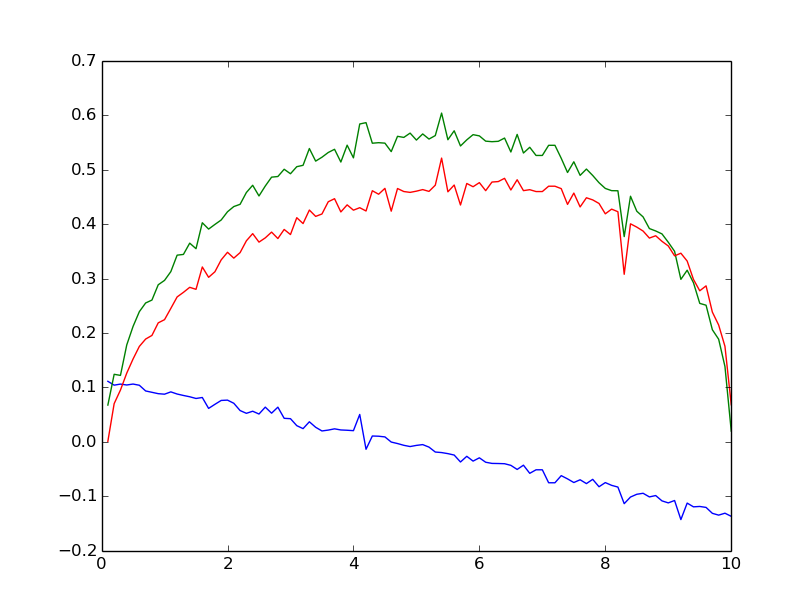
\includegraphics[width = 7.5cm]{figures/swing-traj}\label{fig:badtraj}}\qquad
\subfloat[Après augmentation de la précision]{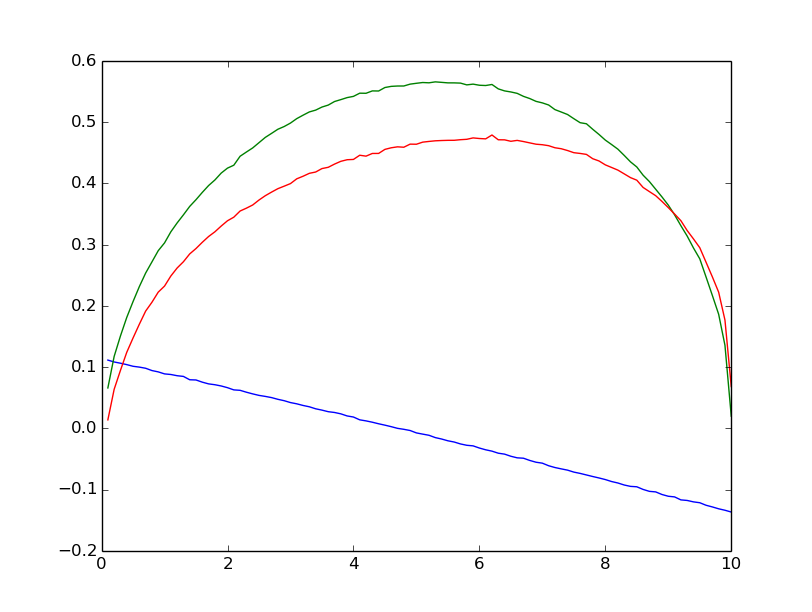
\includegraphics[width = 7.5cm]{figures/swing-traj-better}\label{fig:goodtraj}}\\
\caption{Trajectoire traduite par le solveur de cinématique inverse}
\end{figure}


Ma première hypothèse fut que la précision de l'algorithme d'optimisation était insuffisante. L'étude de la documentation de NLopt a permis d'identifier la manière de régler la précision. Elle était par défaut réglée sur $10^{-3}$, et la passer à $10^{-4}$ a suffit à régler le problème, comme vous pouvez le voir sur la figure \ref{fig:goodtraj} (le code couleur reste identique).

\label{lb:precisionkine} Comme on peut le voir, la précision des calculs est tout à fait suffisante pour notre application, les commandes sont passées en centimètres et la précision est de l'ordre du millimètre. 

\subsection{Module de communication}\label{lb:communication}
Le module de communication se contente d'envoyer les trajectoires aux contrôleurs de trajectoires lancés par le noeud \textit{hexapod\_bringup}. Auparavant appartenant au bloc Hexapod dans les premières versions, il est désormais intégré aux pattes, leur permettant d'effectuer des trajectoires complémentaires de compensation par exemple, indépendamment de la synchronisation globale.

Pour cela, il faut créer un client qui se chargera d'envoyer les trajectoires et d'attendre les réponses du contrôleur de trajectoire lancé d'hexapod\_bringup.Lors de sa création, il faut préciser l'adresse de publication, qui doit correspondre à celle sur laquelle écoute le contrôleur de trajectoires. Dans notre cas, il s'agit d'une chaîne de caractères de la forme :
\begin{equation}
/dynamixel\_controllers/leg\_0\_controller/follow\_joint\_trajectory
\end{equation}
On attend ensuite une réponse du serveur, pour être sûr que celui-ci est démarré. Dans le cas contraire les trajectoires ne pourront être envoyées, et le robot n'effectuera pas les actions commandées. 

Par la suite, il faut demander au client d'envoyer l'objectif à atteindre qui contient notre trajectoire et donc l'ensemble des positions angulaires de commandes avec leurs timings associés. Le procédé est illustré par le listing \ref{lst:sendtraj} 

Il est également possible d'attendre le retour du contrôleur sur le statut de chaque point de la trajectoire, il faut alors appeler cette méthode dans un thread séparé, pour éviter de bloquer toute l'exécution. 

\newpage
\begin{lstlisting}[language=c++,caption={Implémentation de la souscription à un topic ROS}, label={lst:sendtraj}]
//SENDING TRAJECTORY
void Leg::_send_trajectory(const double& duration, const trajectory_msgs::JointTrajectory& trajectory)
{
    control_msgs::FollowJointTrajectoryGoal goal;
    goal.trajectory = trajectory;
    _traj_client->sendGoal(goal);

    //Wait for Results status
    _traj_client->waitForResult(ros::Duration(duration));
    if (_traj_client->getState() != actionlib::SimpleClientGoalState::SUCCEEDED)
        ROS_WARN_STREAM("Trajectory execution for leg_"
            << legNum << " failed with status '"
            << _traj_client->getState().toString() << "'");
}
\end{lstlisting}
\section{Réalisation du bloc hexapod}
\subsection{Création des pattes}
La création des pattes est assez simple, la partie la plus avancée étant la récupération de la chaîne cinématique. Le bloc hexapod se contente par la suite de créer les $n$ pattes, de leur attribuer un numéro et de les stocker en mémoire. 

\subsubsection{Récupération du modèle du robot}\label{lb:creapatte}

Il est possible de charger un arbre cinématique -- équivalent au modèle du robot -- à partir d'un fichier URDF directement, et même si cela représente l'avantage d'être simple, l'inconvénient majeur de cette technique est qu'il faudrait coder en dur le chemin du fichier (ou simplement son nom si on laisse ROS le charger) ce qui veut dire qu'il faudrait éditer le code systématiquement en cas de changement de robot. Ce serait certes plus rapide que de refaire la chaîne cinématique, mais cela n'est toujours pas une bonne façon de faire. 

Une autre solution existe, lors du démarrage du robot par le noeud \textit{hexapod\_bringup}, le fichier de description de ce dernier est chargé dans un paramètre de ros : \textit{\textbackslash robot\_description}. Il est alors possible de récupérer depuis ce dernier une chaîne de caractère contenant l'intégralité du fichier URDF. L'avantage et que nous n'aurons ainsi plus besoin de modifier le code si le modèle du robot change. 

Par la suite, une fonction intégrée à \textit{KDL::Parser} permet de convertir cette chaîne de caractère en un arbre cinétique. La technique utilisée et décrite précédemment est illustrée par le listing \ref{lst:gettree}.

\newpage
\begin{lstlisting}[language=c++,caption={Récupération de l'arbre cinématique depuis robot\_description }, label={lst:gettree}]
KDL::Tree Hexapod::getTreeFromUrdf()
{
    KDL::Tree my_tree;
    std::string robot_desc_string;

    if (!node.getParam("/robot_description", robot_desc_string)) {
        ROS_ERROR("Failed to get /robot_description parameter");
    }
    if (!kdl_parser::treeFromString(robot_desc_string, my_tree)) {
        ROS_ERROR("Failed to construct kdl tree");
    }
    return my_tree;
}
\end{lstlisting}
\subsubsection{Extraction de la chaîne cinématique}

Une fois cet arbre récupéré, il faut en extraire la chaîne cinématique qui nous intéresse. Dans notre cas il s'agit d'extraire une à une les chaînes des pattes, partant du corps du robot et atteignant les capteurs de force. Le listing \ref{lst:getchain} effectue cela. Nous avons maintenant les données nécessaires pour calculer indépendamment les cinématiques de chaque patte.

\begin{lstlisting}[language=c++,caption={Extraction de la chaîne cinématique}, label={lst:getchain}]
 KDL::Chain Hexapod::extractChain(KDL::Tree tree, std::string chainStart,
    std::string chainTip)
{
    KDL::Chain chain;
    if (!tree.getChain(chainStart, chainTip, chain))
        ROS_ERROR_STREAM("Unable to extract Chain " << chainStart << "-->"
                                                    << chainTip << "!");
    return chain;
}
\end{lstlisting}

\subsection{Synchronisation des données d'entrée}
L'objectif ici est de synchroniser les différentes pattes, puis de générer des trajectoires adaptées afin de respecter les contraintes de temps imposées par le paramètre "fréquence"
\subsubsection{Souscription au Topic ROS}
Les données en entrée sont lues sur des Topics \gls{ROS}, à une fréquence choisie lors de la souscription. Cette souscription est en effet accompagnée d'un Timer, qui appellera la fonction choisie à la fréquence choisie. J'ai choisi de mettre à jour directement ces valeurs dès leur arrivée, via des fonctions de callback de la classe Hexapod comme vous pouvez le voir dans le listing \ref{lst:topicROS}. La souscription s'effectuant directement dans la classe exapod après avoir crée l'objet ros::NodeHandle(). Ce dernier doit rester dans le scope au risque de ne plus synchroniser les données. La classe Hexapod transmettant également certaines données directement aux classes Leg si besoin. Les positions angulaires données par les codeurs intégrés aux servos-moteurs sont donc propagées automatiquement là où on en a besoin. Il en va de même pour les valeurs des capteurs de force.  

\begin{lstlisting}[language=c++,caption={Implémentation de la souscription à un topic ROS}, label={lst:topicROS}]
Hexapod::Hexapod(){
    //initialisation de l'hexapod
    joint_states_sub = node.subscribe("/joint_states", 
                                        jointFrequency, 
                                        &Hexapod::jointStatesCallBack, 
                                        this);
}
void Hexapod::jointStatesCallBack(const sensor_msgs::JointState& msg)
{
    //Recuperation et traitement des donnees du message
}
\end{lstlisting}

\subsubsection{Augmenter la fréquence de synchronisation}
Dans un premier temps, en l'absence de capteurs de force, une fréquence de synchronisation élevée n'était pas nécessaire. il suffisait en effet de récupérer la position des servomoteurs une fois par pas, afin de connaître leur position nécessaire au calcul de la trajectoire.  

Le code présenté dans le listing \ref{lst:spinOnce} suffisait alors à récupérer l'information requise, les Callbacks (présentés en \label{lb:callback}) étaient alors appelés une fois par itération. L'instruction \textit{ros::spinOnce()} lançant la synchronisation une seule fois avant de rendre la main, permettant au reste du système d'effectuer ses calculs et opérations.   

\begin{lstlisting}[language=c++,caption={Implémentation simple de la synchronisation de données}, label={lst:spinOnce}]
// Création de l'hexapod
// Assignation des Callbacks
while(ros::ok()){
    ros::spinOnce(); // Effectue la synchronisation 
}
\end{lstlisting}

Il existe bien un outil simple permettant de synchroniser en permanence les données, afin de permettre de tester en continu les valeurs des capteurs de forces. Il s'agit de \textit{ros::Spin()} mais il ne rend pas la main ce qui ne permet pas d'effectuer d'opération supplémentaires. 

La solution se trouve dans un autre outil de ROS, permettant d'effectuer cette mise à jour dans un thread séparé. il s'agit de l'outil \textit{AsyncSpinner}. Il est relativement simple à utiliser et permet de garantir une synchronisation des données à la fréquence définie lors de la souscription au Topic. Son emploi est détaillé dans le listing \ref{lst:asyncspinner}. Il permet de synchroniser en permanence dans d'autres threads, libérant ainsi le thread principal pour nos calculs. C'est la solution qui sera retenue pour synchroniser les données.  

\begin{lstlisting}[language=c++,caption={synchronisation dans un thread séparé}, label={lst:asyncspinner}]
// Creation de l'hexapod
// Assignation des Callbacks
ros::AsyncSpinner spinner(4); // Use 4 threads
spinner.start();
ros::waitForShutdown();
\end{lstlisting}

\subsection{Synchronisation des pattes}
\subsubsection{Ros::Rate}
Peu précis, Ros::Rate encapsule un mécanisme assez simple, qui consiste en l'enregistrement du timeStamp lors de la création de l'objet, ou plus tard, lors de l'appel à la méthode sleep de cette même classe. Il est alors possible de récupérer le temps écoulé depuis l'un de ces événements à n'importe quel moment. Lors de la création de l'objet, on précise une fréquence désirée, qui servira à calculer le temps durant lequel il faut mettre en pause l'exécution pour obtenir la fréquence précédemment définie. Cette pause s'effectuera à l'appel de la fonction sleep.

\begin{lstlisting}[language=c++,caption={Implémentation de Ros::Rate sous \gls{ROS}}, label={lst:rateROS}]
    ros::Rate loop_rate(frequency);
    for (size_t i = 0; i < numOfSteps; i++) {

        ros::spinOnce();

        hexapod->setDuration(1.0 / frequency - loop_rate.cycleTime().toSec());
        hexapod->sync();

        loop_rate.sleep();
    }
    hexapod->relax();
\end{lstlisting}
Après avoir mesuré les temps à l'aide du chrono proposé par c++11, il s'est avéré que cette solution était peu précise, et de surcroît très aléatoire. Il n'etait donc pas envisageable de conserver cette manière de procéder. 

\subsubsection{Ros::Timers + Callbacks}
Meilleure manière de procéder, les Timers fournissent la garantie du respect de la fréquence choisie. L'implémentation n'est pas plus compliquée que Ros::Rate, c'est donc une solution qui devrait être plus mis en avant dans les tutoriels \gls{ROS}. Il suffit ici de créer un timer \gls{ROS} comme l'illustre le code donné en \ref{lst:timersROS}
\newpage
\begin{lstlisting}[language=c++,caption={Implémentation des Timers sous \gls{ROS}}, label={lst:timersROS}]
void hexapodSyncCallBack(const ros::TimerEvent& e)
{
    hexapod->setDuration(1 / frequency); //Definit la duree de la trajectoire
    hexapod->sync(); //Lance le calcul des trajectoires 
    steps++;
}
ros::Timer timer = n.createTimer(ros::Duration(1 / frequency), 
                                    hexapodSyncCallBack);
while (steps < numOfSteps) {
    ros::spinOnce();
}
hexapod->relax();
\end{lstlisting}
Il est nécessaire d'ajouter un ros::Spin(), afin que les timers puissent fonctionner. Dans notre cas, il est même préférable d'utiliser ros::SpinOnce(), qui n'est pas une boucle infinie, et qui à l'avantage de nous permettre de limiter le nombre de pas à exécuter à chaque fois que l'on lance le contrôleur. Ce qui est fort pratique quand la zone de test est limitée, afin d'éviter une malencontreuse rencontre avec l'enceinte de l'arène. 

\newpage
\section{Modèle du nouveau robot}\label{lb:xacro}
Comme nous avons pu le voir, notamment dans la partie \ref{lb:kinematics} et dans la parte \ref{lb:rosdart}, le modèle du robot joue un rôle primordial dans notre contrôleur. Sans lui impossible de tester le robot en simulation, impossible de déplacer les pattes. De plus, une simple erreur dans le modèle peut avoir des conséquences néfastes. En effet, une erreur sur les dimensions des pattes peut conduire à un calcul de cinématique éloigné de la vérité, provoquant ainsi des commandes sans rapport avec la réalité physique du robot. On pourrait donc lui demander de passer à travers son corps ou autre, provoquant dans le meilleur des cas une légère erreur de position des pattes et dans le pire des cas des collisions avec les autres composantes du robot. 
\subsection{organisation des scripts}
Chaque robot comprend quatres modules\footnote{Ces modules sont disponibles ici : \url{https://github.com/resibots/hexapod_ros/tree/marta-and-pexod-optoforce/hexapod_description/urdf/modules}} permettant de générer le modèle du robot :
\begin{itemize}
    \item Principal, nommé avec le nom du robot
    \item body contenant la description du corps
    \item legs contenant les pattes et leurs positions
    \item leg  contenant la description d'une patte
\end{itemize}

\subsubsection{Module principal}
Le module principal à pour but d'appeler les autres scripts, il contient aussi les propriétés xacro. Ces propriétés sont des ensembles clé-valeur et leur syntaxe est donnée en \ref{lst:xacroparam}. L'exemple donné défini par exemple l'épaisseur du premier segment d'une patte.

\begin{lstlisting}[language=XML,caption={Couple clé-valeur correspondant à un paramètre},label={lst:xacroparam}]
<xacro:property name="leg1_width" value="0.02"/>
\end{lstlisting}

Afin de charger les autres scripts, on utilisera la fonction de recherche de ROS nommée \textit{find()} permettant de trouver un package ros, ce qui permet d'être indépendant du chemin réel sur la machine, ce qui est indispensable afin de rendre le programme portable. La syntaxe est illustrée par le listing \ref{lst:xacroload}.=, dans lequel le script de génération du corps du robot est chargé.

\begin{lstlisting}[language=XML,caption={Chargement d'un autre script},label={lst:xacroload}]
<!-- Load xacro modules/parts of the robot -->
<xacro:include filename="$(find hexapod_description)/urdf/modules/body.xacro"/>

\end{lstlisting}

 
\subsubsection{Module body}
Le module body défini le lien de base, sur lequel toutes les pattes seront fixées. Il comporte aussi les informations d'inertie du corps. Nulle nécessité de le modifier pour nous. Il sera néanmoins modifié par Dorian Goepp afin de respecter au mieux le visuel du robot et de pouvoir distinguer l'avant du robot.

\subsubsection{Module Legs}
Le module leg, comme annoncé précédemment, positionne et crée les pattes. Le listing \ref{lst:xacrocreapatte} montre la manière de créer une patte, lui donnant les paramètres dont elle a besoin pour générer tous ses composants. Ce module ne sera pas non plus modifié dans le cadre du stage.
\begin{lstlisting}[language=XML,caption={Création d'une patte},label={lst:xacrocreapatte}]
<xacro:leg index="0" xPos="${-body_length/2}"yPos="${body_width/2}"sign="1"/>
\end{lstlisting}

\subsubsection{Module leg}
C'est le module le plus complet de tous, il contient tout ce qu'il faut pour générer le visuel, la géométrie pour les collisions et les calculs, les poids et dimensions de chaque composant des pattes. Plusieurs modifications sont à effectuer sur ce script afin d'ajouter des fonctionnalités à l'ensemble du système. 

Dans un premier temps, la géométrie des pattes a été mise à jour par Dorian Goepp, afin de correspondre au design des nouvelles pattes. Détaillons maintenat les autres modifications effectuées. 
\subsection{Modifications pour les calculs cinématiques}\label{lb:majurdfkinetic}

KDL a besoin de la chaîne cinématique pour effectuer la cinématique directe, qui est indispensable pour connaître la position actuelle de l'extrémité de la patte mais aussi pour les calculs de cinématique inverse présentés en \ref{lb:kinematics}. Or cette chaîne cinématique est extraite du fichier de description. 

Lors du calcul de cinématique, KDL prends pour extrémité de la chaîne le dernier joint et non le dernier lien. Cela pose problème car dans notre cas, le denier joint est situé au niveau de la cheville, qui est réellement loin de l'extrémité réelle de la patte. Après avoir cherché la bonne manière de faire dans la documentation de KDL, il s'est avéré qu'il fallait ajouter un nouveau lien attaché au bout de la chaîne cinématique par un joint qui servira alors de référence. 

Le listing \ref{lst:xacrodummyfix} contient l'ajout effectué en extrémité de chaîne. On y définit l'origine du joint qui servira de référence pour les calculs cinématiques. Après vérification, les calculs obtenus sont désormais corrects. 
\clearpage
\begin{lstlisting}[language=XML,caption={Correction de l'extrémité de la patte},label={lst:xacrodummyfix}]
<joint name="dummy_joint_${index}_fix" type="fixed">
    <parent link="leg_${index}_3"/>
    <child link="force_sensor_${index}"/>
    <origin rpy="${-sign*PI_2} 0 0" xyz="0 ${sign*leg3_length} ${leg3_dist}"/>
</joint>
<link name="dummy_link_${index}"/>
        
\end{lstlisting}


\subsection{Modifications pour RosDart}
Le fichier de description généré pars les scripts xacro était utilisable en l'état, mais ne permettait pas le contrôle des servomoteurs ce qui empêchait toute simulation pertinente. En effet, il manquait une cartographie entre les servomoteurs et les liens qui leurs étaient associés. Dans le but d'indiquer ces paires dans le fichier de description, il faut ajouter des transmissions. La syntaxe est assez simple, elle est décrite dans le listing \ref{lst:xacrotrans}. Dans cet exemple, nous ajoutons une transmission au niveau de la hanche. Nous lions le joint $body_leg_x$ au servomoteur $moteurx1$. 

\begin{lstlisting}[language=XML,caption={Ajout des transmissions},label={lst:xacrotrans}]
<transmission name="tran${index}1">
    <type>transmission_interface/SimpleTransmission</type>
    <joint name="body_leg_${index}">
        <hardwareInterface>PositionJointInterface</hardwareInterface>
    </joint>
    <actuator name="motor${index}1">
        <hardwareInterface>PositionJointInterface</hardwareInterface>
        <mechanicalReduction>1</mechanicalReduction>
    </actuator>
</transmission>

\end{lstlisting}

Une fois ces modifications effectuées pour les trois servomoteurs de chaque patte, il est devenu possible de contrôler le robot en simulation. 

\subsection{Modifications pour les capteurs de force}
Afin de récupérer les valeurs des capteurs de force en simulation, Konstantinos Chatzilygeroudis a ajouté un nouveau type de balise permettant de préciser la position du capteur ainsi que le topic ROS sur lequel l'on souhaite qu'il publie ses données. Il faut positionner ce lien à l'extrémité de la patte. 

Or il se trouve que l'on a déjà ajouté un lien précédemment pour les besoins de la cinématique, il suffit donc d'exploiter se lien afin d'y greffer le capteur.
\clearpage

\begin{lstlisting}[language=XML,caption={Modifications et ajout du capteur},label={lst:xacrocapteur}]
<joint name="force_sensor_${index}_fix" type="fixed">
    <parent link="leg_${index}_3"/>
    <child link="force_sensor_${index}"/>
    <origin rpy="${-sign*PI_2} 0 0" xyz="0 ${sign*leg3_length} ${leg3_dist}"/>
</joint>
<link name="force_sensor_${index}"/>
<dart_sensor type="force">
  <link>force_sensor_${index}</link>
  <frequency>1000</frequency>
  <topic>optoforce_${index}</topic>
</dart_sensor>

\end{lstlisting}


\chapter{Résultats et performances}


\section{Résultats Obtenus}
\subsection{Une solution de cinématique inverse performante}
Comme présenté précédemment en \ref{lb:precisionkine}, les résultats obtenus sont très satisfaisants et notre solution de cinématique inverse trouve toujours une solution, même dans le cas ou la position demandé n'est pas atteignable. 

L'algorithme d'optimisation va alors trouver la solution la plus proche possible de l'objectif souhaité, tout en avertissant l'utilisateur que la solution n'est pas atteignable. Il est même possible d'afficher la distance d'erreur. L'algorithme est en effet programmé pour s'arreter après $x$ itérations, permettant de ne pas consommer trop de temps machine.

Le tableau \ref{tab:perf} récapitule les performances des différents algorithmes. Le temps moyen d'une itération correspond au temps nécessaire au calcul de la cinématique inverse d'un point, celui pour les six pattes correspond au temps nécessaire pour calculer un point par patte, et la dernière colonne donne la fréquence maximale d'emploi de l'algorithme -- c'est à dire combien de points par seconde et par pattes peut on calculer en exploitant toute la puissance disponible. 

Ces benchmarks ont été réalisés sur la machine qui m'a été fournie avec une précision réglée sur $10^{-3}$ qui représente l'erreur tolérée à laquelle l'algorithme s'arrêtera. Cette machine est bien moins puissante que la machine sur laquelle le contrôleur tournera réellement, ce qui garantit son bon fonctionnement.

\begin{table}[]
\centering
\begin{tabular}{|l|l|l|l|}
\hline
Algorithme       & Temps moyen d'une itération en us  & temps pour les 6 pattes & Fréquence max Hz \\ \hline
Cobyla     & 400                                                               & 2400                    & 416,6666667      \\ \hline
BOBYQA     & 100                                                               & 600                     & 1666,666667      \\ \hline
NEWUOA     & 370                                                               & 2220                    & 450,4504505      \\ \hline
PRAXIS     & 180                                                               & 1080                    & 925,9259259      \\ \hline
NELDERMEAD & 70                                                                & 420                     & 2380,952381      \\ \hline
SBPLX      & 110                                                               & 660                     & 1515,151515      \\ \hline
\end{tabular}
\caption{Tableau comparatif des performances (réalisé sur 10 000 itérations)}
\label{tab:perf}
\end{table}

Il va sans dire que nous avons choisi l'algorithme le plus rapide, \textit{NELDERMEAD}\footnote{La méthode de Nelder-Mead est un algorithme d'optimisation non-linéaire qui a été publiée par John Nelder et Mead en 1965. C'est une méthode numérique heuristique qui cherche à minimiser une fonction continue dans un espace à plusieurs dimensions.}. Cet algorithme présente l'avantage d'être efficace dans le cas d'une fonction non dérivable, avec un problème de faible dimension (c'est le cas ici car $N=3$). Même après avoir augmenté la précision du solveur, le temps nécessaire pour calculer un point ne dépasse pas les 100 us, ce qui reste totalement raisonnable pour notre application.

Cette solution de calcul de cinématique inverse permet donc de générer de nombreuses trajectoires selon nos besoins.

\subsection{Un Contrôleur facilement adaptable}

L'emploi du pattern strategy permet de créer et d'intégrer rapidement des comportements additionnels apportant une grande adaptabilité à l'ensemble. Cela permettra également de suivre différents axes d'amélioration en simultané, en changeant par exemple la procédure en cas de contact pour effectuer le contrôle de la force évoqué dans l'état de l'art.  

\subsection{Un contrôleur omnidirectionnel}
La capacité du contrôleur à évoluer dans toutes les directions en suivant un simple vecteur de commande est un avantage en soi. Le précédent contrôleur de l'équipe ne proposait en effet qu'une marche simple, les comportements omnidirectionnels devaient êtres appris. Cela représente un gain de temps et d'énergie non négligeable. 

Cette capacité omnidirectionnelle permet également de dégager de nouveaux comportements, par exemple aborder un terrain difficile en diagonale peut permettre de gagner en efficacité. 

\subsection{Un contrôleur plus robuste ?}

Les premiers tests ont permis de déterminer que le robot avait moins tendance à se déstabiliser lors du franchissement d'un obstacle. En effet, le fait de stabiliser son assiette et de suivre le mouvement lors de la détection d'un contact avec un obstacle évite au robot de se surélever en continuant à pousser sur la patte forçant sur l'obstacle. 

Ces tests ont été réalisés dans l'arène de l'équipe (visible en figure \ref{fig:arene}, préparée pour l'occasion avec des obstacles divers et variés afin de simuler un environnement difficile. 

Le principal problème rencontré se situe dans la reproduction des conditions de l'expérience. En effet, afin de mesurer l'apport de la prise en compte des capteurs dans la capacité du robot à évoluer en terrains difficiles, nous effectuons un essai avec les capteur et un essai sans. Il est difficile de positionner le robot exactement dans la même position initiale, ce qui change fortement l'angle d'attaque du robot et influe donc sur sa capacité à franchir le parcours.

L'idée serait à terme d'essayer de positionner le robot avant l'expérience grâce au système de suivi infrarouge de l'arène de l'équipe. Cela permettrait à la fois d'obtenir des conditions quasi-similaires, mais également d'effectuer des mesures concrètes de la performance des essais avec et sans capteurs. 

Ces essais sont déjà en cours et seront poursuivis d'ici à la fin du stage, afin de fournir à l'équipe une information plus précise concernant les résultats obtenus par le nouveau contrôleur. 

\begin{figure}
    \centering
    \includegraphics[width=\textwidth]{figures/terrain}
    \caption{Terrain de test}
    \label{fig:arene}
\end{figure}

\section{Axes d'amélioration}
Il existe de nombreux progrès réalisables sur la version actuelle du contrôleur. Cette liste d'améliorations est potentiellement infinie, c'est la raison pour laquelle ne seront présentés que les principaux axes.

\subsection{Contrôle de la force}
Comme exposé dans l'état de l'art en \ref{lb:ctrlforce}, implémenter un contrôle plus précis de la force peut s'avérer intéressant pour garantir un bonne stabilité de la plateforme. Un asservissement de la force de chaque patte peut éventuellement être effectué afin d'obtenir une stabilité optimale. Il suffirait alors de mesurer la force, et d'ajuster la position de la patte en conséquence. l'éloignant de point de contact dans la direction de la force mesurée si celle ci est trop forte, ou au contraire pousser dans la direction opposée de la force si celle-ci n'est pas suffisante. 
\subsection{Mapper les forces}
Si asservir les forces aux extrémités des pattes peut s'avérer intéressant, créer une carte des force exercées et réagir aux perturbations extérieures en contrôlant l'ensemble des pattes de concert optimisant ainsi la posture et les réactions locales. 

\subsection{Permettre de modifier les points neutres des pattes}
Une piste intéressante de compensation de dommage pourrait consister à déplacer les positions neutres des pattes, utilisées pour calculer l'objectif de chaque pas présenté en \ref{lb:corrvect}. Déplacer ce centre permettrait donc de compenser l'équilibre du robot dans le cas d'une perte de patte. Il permettrait également de générer une variété plus riche de comportements, ce qui peut représenter un intérêt certain pour l'équipe dans le cadre de l'utilisation de leurs algorithmes d'apprentissage.

Mise à jour : cette fonctionnalité a été intégrée, toutefois sans mécanisme intelligent permettant d'adapter automatiquement ces points de référence. Cela permet par exemple de modifier la hauteur du robot, ce qui influe beaucoup sur sa capacité de franchissement ainsi que sur sa stabilité.

\subsection{Utiliser la centrale inertielle}
L'apport du traitement des données de la centrale inertielle permettrait de commander les pattes en fonction de l'assiette du robot. On pourrait par exemple facilement ajuster la hauteur de chaque patte afin d'ajuster cette assiette, en fonction du comportement désiré. 

Cela permettrait également de compenser une défaillance, dans le cas d'une patte avant sectionnée, il serait possible d'incliner l'assiette du robot vers l'arrière afin de conserver une posture stable en repositionnant le centre de masse à l'intérieur du polygone de support des pattes. 

Cette centrale inertielle permettrait également de détecter un mouvement brusque comme une chute, qui associé à un grand changement de force appliqué en extrémité de patte, permettrait de savoir quelle patte est en train de glisser et donc quelle patte il faut tenter de stabiliser.

Un autre apport potentiel serai la prise en compte de l'orientation du robot pour les calculs de trajectoires. Au lieu de calculer comme c'est le cas actuellement sans prendre en compte sa rotation par rapport à la gravité, nous pourrions adapter les trajectoires des pattes afin de maintenir celles-ci parallèles à la gravité. Cela permettrait d'augmenter grandement la stabilité de la plateforme. 

\subsection{Planification locale du positionnement des pattes}
Utiliser un mécanisme de vision permettrait également de faire du planning, pas pour trouver le chemin à effectuer, mais pour savoir où poser sa patte de manière sure. cela permettrait d'éviter de glisser, du moins dans la plupart des cas. L'autre avantage de l'ajout d'une cartographie locale est l'obtention d'un modèle de l'environnement, redonnant de l'intérêt aux approches basées sur le modèle telles que les \gls{MPC}. 

\subsection{Combiner plusieurs de ces approches}
Bien entendu, de nombreuses améliorations sont indépendantes, mais peuvent parfois êtres couplées, afin d'obtenir un contrôleur encore et toujours plus robuste, encore plus fiable. 

\section{Respect du planning prévisionnel}
\subsubsection{Planning prévisionnel}
Étant néophyte dans le domaine ciblé par le stage et n'ayant par conséquence que peu d'expérience, il n'a pas été évident de planifier correctement l'ensemble du projet. Ce planning a donc été réalisé après la phase de prise en main et d'état de l'art. 
\begin{figure}[h]
    \centering
    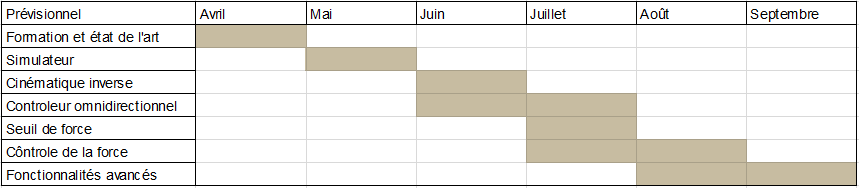
\includegraphics[width=\textwidth]{figures/prev}
    \caption{Planning prévisionnel }
    \label{fig:prev}
\end{figure}

Comme vous pouvez le voir sur la figure \ref{fig:prev}, la réalisation des composants indispensables a été planifiée en premier, à savoir le module de cinématique inverse et le contrôleur omnidirectionnel. Le plan était d'atteindre ses objectifs, puis de finaliser une première version basique du contrôleur utilisant un seuil de force pour détecter un contact. 

Par la suite, il était prévu d'ajouter de plus en plus de fonctionnalités tels qu'un contrôle avancé de la force appliquée aux pattes et puis si possible un \gls{MPC}.
\newpage
\subsubsection{Planning réel}\label{lb:planningreel}

Il n'est jamais évident de prévoir exactement le déroulement d'un projet. Mais si l'on regarde la figure \ref{fig:reel}, on constate que mise à part le retard important engendré par la cinématique inverse, le reste des jalonnements prévus s'est enchaîné dans l'ordre prévu.

Toutes les fonctionnalités prévues n'ont pu êtres implémentées, mais la version actuelle du contrôleur et fonctionnelle, et les améliorations possibles sont décrites ici-même. De plus, le stage n'est pas encore fini, et il reste suffisamment de temps pour en ajouter quelques unes. 

\begin{figure}[h]
    \centering
    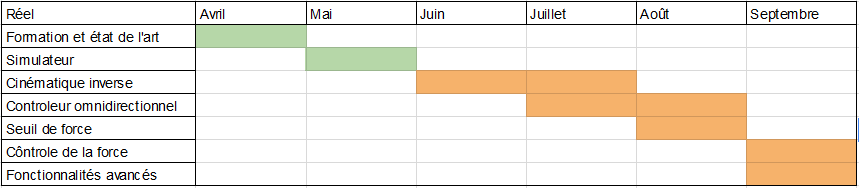
\includegraphics[width=\textwidth]{figures/reel}
    \caption{Planning réel }
    \label{fig:reel}
\end{figure}
\section{Ressenti personnel}
\subsection{Un accueil Chaleureux}
Dès mon arrivée et jusqu'au terme de ce stage, l'accueil de l'équipe \gls{LARSEN} fut réellement amical. Partager ensemble les repas du midi a créé de nombreuses occasion de discuter de sujets diverses et variés et de découvrir le rôle et les investigations de chacun.
\subsection{Un environnement enrichissant}
Lors du déroulement de ce stage ont eu lieu des conférences enrichissantes dans le cadre des 40 ans du \gls{LORIA}. C'est une chance d'avoir pu assister aux démonstrations effectuées par des précurseurs dans leur domaine. 

\subsection{Un domaine intéressant}
La robotique est un domaine qui m'a toujours intéressé, et plus particulièrement l'apprentissage. Ce stage a donc représenté pour moi une réelle opportunité de découvrir en direct l'application concrète d'algorithmes d'apprentissage, et d'avoir de surcroît des explications quand à leur fonctionnement particulier. Et ce grâce à de nombreux échanges avec mes collègues. 
\subsection{Des difficultés rencontrées}
Comme nous avons pu le voir dans la partie \ref{lb:planningreel}, toutes les étapes prévues n'ont pu être réalisées au terme de ce stage. Le robot est certes fonctionnel, mais beaucoup d'améliorations supplémentaires auraient pu êtres implémentées. 

En effet, les difficultés rencontrées lors de la réalisation des calculs cinématiques on grandement retardé la mise en oeuvre du reste du contrôleur. Cette tâche semblait facile et à demandé bien plus d'énergie et d'investissement que prévu, mais avec ma faible expérience en la matière, il était difficile de voir venir ces déconvenues.

\subsection{Une légère déception}
Ce retard s'étant reporté sur l'ensemble du projet, il n'a pas été possible d'implémenter les fonctionnalités plus avancées imaginées lors de ce stage. Le fait de ne pas avoir pu travailler sur ces ajouts améliorés me laisse un goût amer, car cela constitue la partie la plus gratifiante du stage. Même si tout le travail préliminaire est indispensable et conséquent, c'est la partie la plus passionnante. 

\subsection{Des résultats encourageants}
Néanmoins, les résultats obtenus sont encourageants, et malgré le fort retard provoqué par la cinématique inverse, le projet à quand même aboutit à un contrôleur omnidirectionnel fonctionnel, et prenant en compte les retours des capteurs afin de s'adapter au terrain. 

Il reste toutefois quelques jours de stage et quelques améliorations à explorer, ce qui est encourageant.

\chapter{Conclusion}

Quelques jours avant le terme du stage, l'objectif principal de détermination et d'implémentation d'un contrôleur réactif pour hexapod est rempli. Cela a été rendu possible dans un premier temps par une analyse détaillée de la problématique, puis une recherche méthodique de solutions potentielles, à travers la lecture de nombreuses publications scientifiques sur le sujet. 

Après avoir acquis une idée plus précise des possibilités offertes, un choix raisonnable a permis d'opter pour une solution atteignable, autant sur le point pratique dans son implémentation que dans ses concepts théoriques, permettant de maîtriser le projet jusqu'à son terme et ce malgré quelques écueils.

Des difficultés réellement enrichissantes sont survenues au fur et à mesure de l'avancement du projet. La principale ayant sans nul doute été la réalisation du module de cinématique inverse, qui n'avait pas été perçu comme obstacle potentiel. Après avoir échoué à faire fonctionner des librairies -- pourtant spécialisées -- dans notre contexte particulier, il a fallu faire preuve de persévérance afin de concevoir et développer ma propre solution, qui s'avère même plus avantageuse sur certains points (voir \ref{lb:kinematics}). Cette expérience a donc représenté pour moi une réelle leçon. 

L'adoption d'une méthode de tests et validations successifs a permis d'avancer de manière saine et sécurisée dans le projet. Les fonctionnalités ont été ajoutées au fur et à mesure pour aboutir à une version fonctionnelle. 

Il reste de nombreuses améliorations possibles, et je tenterais autant que faire ce peut de pousser le projet encore plus loin dans les jours à venir. La réalisation de mesures de performances étant toujours en cours, ces dernières seront analysées avant le départ du stage afin de fournir une analyse complète de l'apport réel des travaux réalisés durant ce stage.

D'un point de vue personnel, je dois avouer une certaine déception de ne pas avoir pu à ce jour implémenter les fonctionnalités identifiées et théoriquement préparées. 

Ce stage a représenté une expérience réellement enrichissante, me donnant un accès au monde de la recherche et à nombre de ses connaissances. Qu'elles viennent de l'accès aux publications scientifiques, du suivi de conférences --menées par des experts de leur domaine-- ou encore de l'apport journalier de mes collègues, ces sources d'informations n'ont fait que renforcer mon intérêt pour la science, et plus particulièrement pour la robotique.
\newpage
Le monde de la recherche me plaît, et j'aimerais si l'occasion s'en présente continuer mes études dans cette voie. A la suite de ce stage, j'ai encore quelques doutes quant à ma capacité réelle à poursuivre en thèse. C'est dans ce contexte flou que je recherche actuellement les opportunités s'offrant à moi, qui me permettraient de continuer à en apprendre toujours plus dans le domaine. J'envisage actuellement d'effectuer une mission à l'étranger, afin de voyager et d'y découvrir d'autres cultures, d'autres horizons, ce qui m'aidera sans aucuns doutes à mieux cerner l'orientation que je veux donner à ma vie, aussi bien personnelle que professionnelle. 

 
\cleardoublepage
\renewcommand{\tocbibname}{Bibliographie / Webographie}
\nocite{*}
\bibliography{biblio}
\bibliographystyle{plain}

\cleardoublepage

\printglossary
\printglossaries
\cleardoublepage

\listoffigures
\cleardoublepage

\lstlistoflistings
\cleardoublepage

\appendix
\chapter{Organigramme LORIA}

\begin{figure}[h]
    \centering
    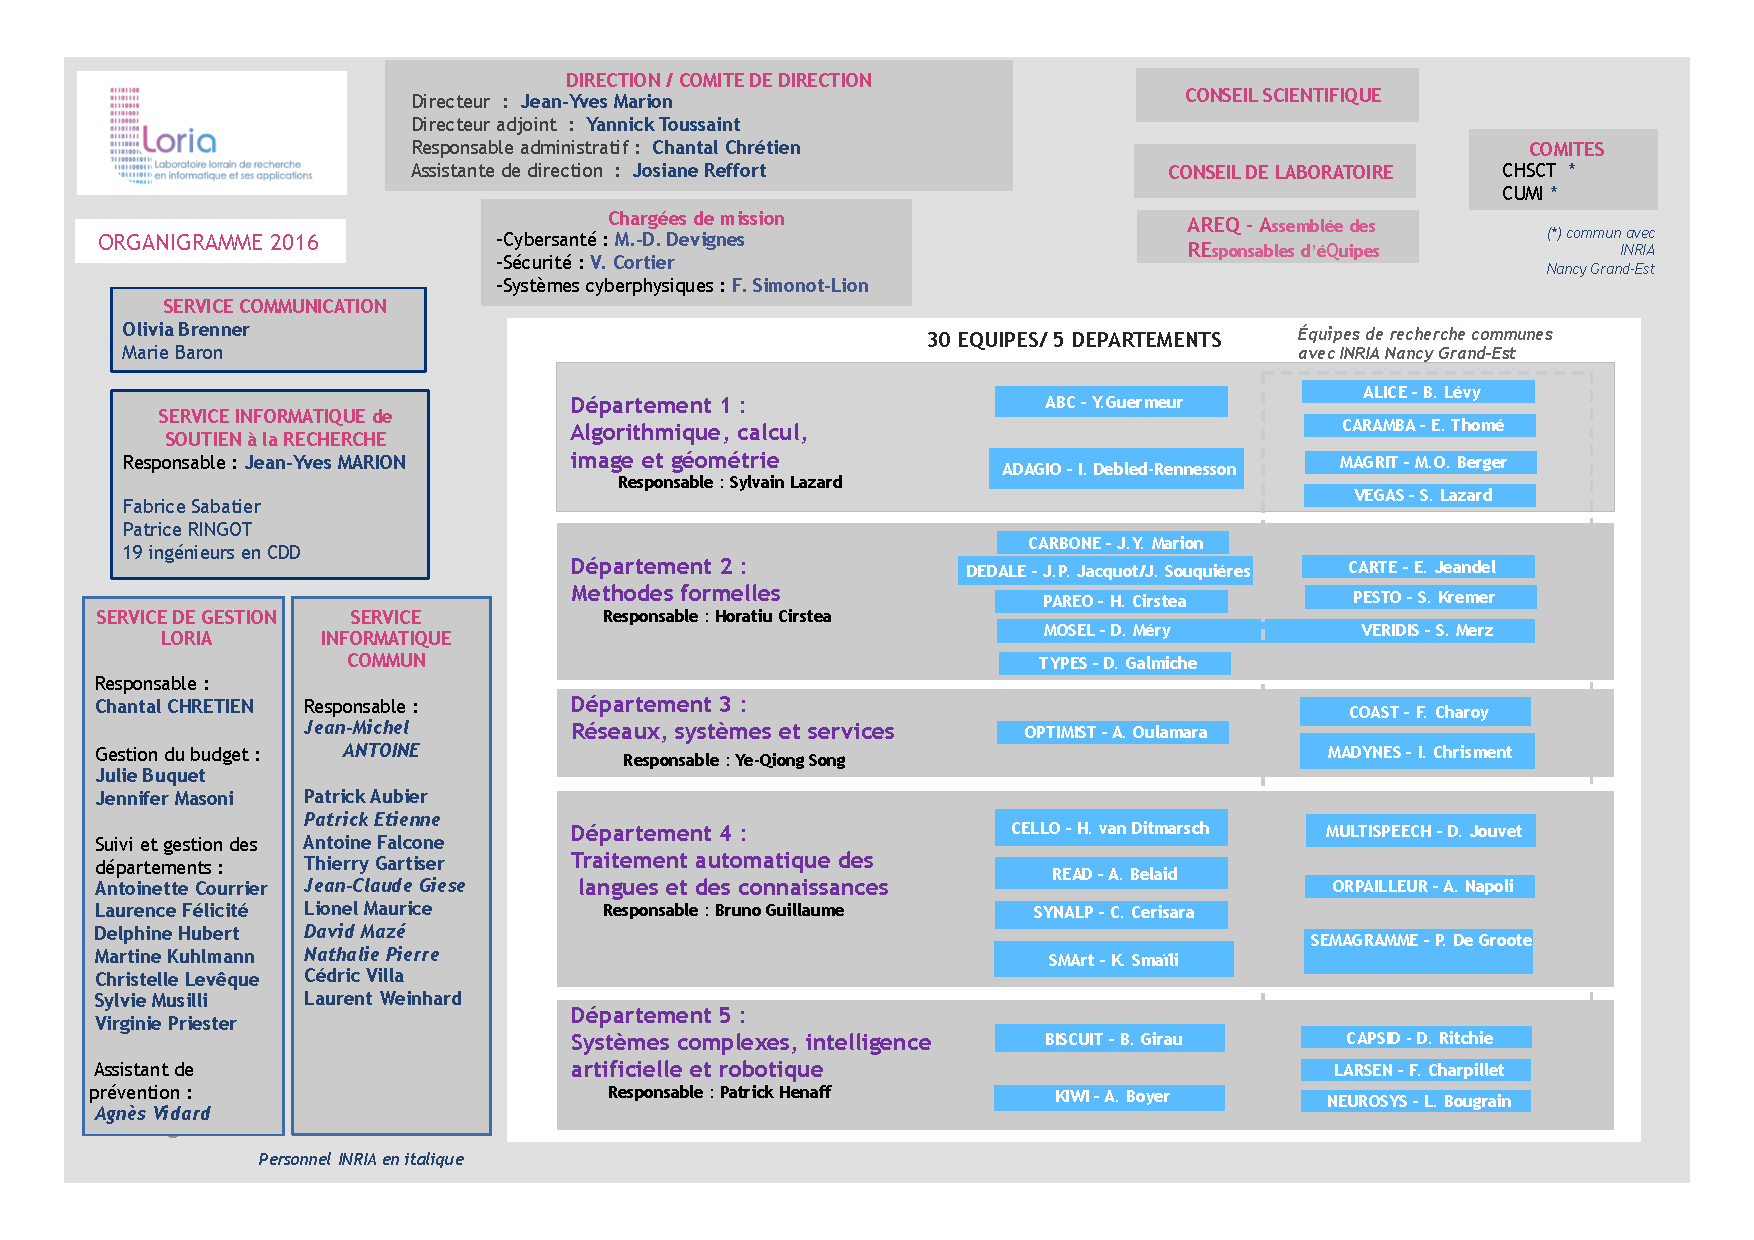
\includegraphics[scale=0.6,angle=90]{figures/orga-loria}
    \caption{Organigramme du LORIA}
    \label{fig:orgaLoria}
\end{figure}
\clearpage

\chapter{Example de fichier URDF}\label{lb:urdf}
\begin{lstlisting}[language=xml,caption={Exemple de fichier URDF, ici une partie de la jambe de notre robot}, label={lst:exempleURDF}]
<joint name="leg_2_1_2" type="revolute">
    <parent link="leg_2_1"/>
    <child link="leg_2_2"/>
    <limit effort="30.0" lower="-0.78539816339" upper="0.78539816339" velocity="7.0"/>
    <origin rpy="0 0 0" xyz="0 0.06 0"/>
    <axis xyz="1 0 0"/>
    <dynamics damping="0.0"/>
  </joint>
  <link name="leg_2_2">
    <visual>
      <origin rpy="1.57079632679 0 0" xyz="0.01 0.0425 0"/>
      <geometry>
        <cylinder length="0.085" radius="0.02"/>
      </geometry>
      <material name="Blue"/>
    </visual>
    <collision>
      <origin rpy="1.57079632679 0 0" xyz="0.01 0.0425 0"/>
      <geometry>
        <box size="0.02 0.02 0.085"/>
      </geometry>
    </collision>
    <inertial>
      <!-- CENTER OF MASS -->
      <origin rpy="1.57079632679 0 0" xyz="0.01 0.0425 0"/>
      <mass value="0.184"/>
      <!-- box inertia: 1/12*m(y^2+z^2), ... -->
      <inertia ixx="0.000116916666667" ixy="0" ixz="0" iyy="0.000116916666667" iyz="0" izz="1.22666666667e-05"/>
    </inertial>
  </link>
\end{lstlisting}
\newpage
\section*{Résumé}
\addcontentsline{toc}{chapter}{Résumé}
Ce mémoire relate l'expérience vécue lors d'un stage de fin d'études effectué à l'\gls{INRIA} dans le but d'obtenir le diplôme d'ingénieur délivré par Telecom Nancy. L'objectif de ce stage est la réalisation d'un ou plusieurs contrôleurs pour hexapode, devant prendre en compte des capteurs de force. Seront présentés dans cet ouvrage les outils, méthodes et solutions qui ont permis d'atteindre l'objectif fixé. Un état de l'art tente de donner les bases théoriques et les raisons du choix effectué, privilégiant les approches pragmatiques aux approches biomimétiques. Le contrôleur réalisé s'appuie sur des pattes indépendantes, capables de générer leur propre trajectoire dans l'espace cartésien, ainsi qu'un module de cinématique inverse chargé de convertir ses trajectoires en ordres pour les actionneurs des pattes. Un module de contrôle omnidirectionnel sera chargé quant à lui de donner les objectifs aux pattes ainsi que de s'assurer de leur bonne synchronisation. Le contrôleur ainsi réalisé permet d'adopter un comportement plus stable dans des environnements difficiles. Seront donc présentés les différents modules, comprenant une partie théorique expliquant leur fonctionnement et une partie détaillant leur implémentation. Par la suite, un chapitre détaillera les résultats obtenus ainsi qu'une description des expérimentations ayant permis de les obtenir.
{\bf Mots-clés : Hexapode, locomotion, robotique, cinématique, marche omnidirectionnelle}

\section*{Abstract}
\addcontentsline{toc}{chapter}{Abstract}
This paper describes the experience during an internship conducted at the \ gls {INRIA} in order to get the engineering degree from Telecom Nancy. The objective of this course is the design and realization of one or more controllers for hexapod, who should take force sensors into account. Will be presented in this work the tools, methods and solutions that have allowed to reach the target. A state of the art will attempts to provide the theoretical basics and reasons why favoring pragmatic approaches to biomimetic approaches. Realized controller relies on independent legs, capable of generating their own path in Cartesian space, an inverse kinematics module responsible for converting those trajectory in commands for the actuators of the legs. Omnidirectional control module will be responsible for giving each leg goals as well as ensure their proper synchronization. The thus achieved controller allows to adopt a more stable performance in harsh environments. Will thus be presented the different modules, with a theoretical part explaining their operation and some detailing their implementation. Subsequently, a chapter will detail the results and a description of experiments that enabled to get them.
{\bf Keywords : Hexapod, loccomotion, robotics, kinematics, omnidirectional walking }
\end{document}